%% LyX 2.4.3 created this file.  For more info, see https://www.lyx.org/.
%% Do not edit unless you really know what you are doing.
\documentclass[journal,article,submit,pdftex,moreauthors]{Definitions/mdpi}
\usepackage[utf8]{inputenc}
\usepackage{float}
\usepackage{url}
\usepackage{amsmath}
\usepackage{graphicx}

\makeatletter

%%%%%%%%%%%%%%%%%%%%%%%%%%%%%% LyX specific LaTeX commands.

\Title{Improving the performance of constructed neural networks with a pre-train
phase}

\TitleCitation{Improving the performance of constructed neural networks with a pre-train
phase}

\Author{Ioannis G. Tsoulos$^{1,*}$, Vasileios Charilogis$^{2}$, Dimitrios
Tsalikakis$^{3}$}

\AuthorNames{Tsoulos, I.G., Charilogis, V., \textbackslash\& Tsalikakis, D. }

\AuthorNames{Ioannis G. Tsoulos, Vasileios Charilogis and Dimitrios Tsalikakis. }

\AuthorCitation{Tsoulos, I.G.; Charilogis, V.; Tsalikakis, D. }


\address{$^{1}$\quad{}Department of Informatics and Telecommunications,
University of Ioannina, Greece; itsoulos@uoi.gr\\
$^{2}$\quad{}Department of Informatics and Telecommunications, University
of Ioannina, Greece; v.charilog@uoi.gr\\
$^{3}\quad$Department of Engineering Informatics and Telecommunications,
University of Western Macedonia, 50100 Kozani, Greece; tsalikakis@gmail.com}


\corres{Correspondence: itsoulos@uoi.gr}


\abstract{A multitude of problems in contemporary literature are addressed
using machine learning models, the most widespread of which are artificial
neural networks. Furthermore, in recent years, evolutionary techniques
have emerged that identify both the architecture of artificial neural
networks and their corresponding parameters. Among these techniques,
one can also identify the artificial neural networks being constructed,
in which the structure and parameters of the neural network are effectively
identified using Grammatical Evolution. In this work, a pre-training
stage is introduced in which an artificial neural network with a fixed
number of parameters is trained using some optimization technique
such as the genetic algorithms used here. The final result of this
additional phase is a trained artificial neural network which is introduced
into the genetic population used by Grammatical Evolution in the second
phase. In this way, finding the overall minimum of the error function
will be significantly accelerated, making the second phase method
more efficient. The proposed work was applied on a series of classification
and regression problems found in the recent literature and it was
compared against other methods used for neural network training as
well as against the original neural network construction method. }


\keyword{Neural networks; Grammatical Evolution; Genetic algorithms.}

\DeclareTextSymbolDefault{\textquotedbl}{T1}
%% Because html converters don't know tabularnewline
\providecommand{\tabularnewline}{\\}

%%%%%%%%%%%%%%%%%%%%%%%%%%%%%% Textclass specific LaTeX commands.
\newenvironment{lyxcode}
	{\par\begin{list}{}{
		\setlength{\rightmargin}{\leftmargin}
		\setlength{\listparindent}{0pt}% needed for AMS classes
		\raggedright
		\setlength{\itemsep}{0pt}
		\setlength{\parsep}{0pt}
		\normalfont\ttfamily}%
	 \item[]}
	{\end{list}}

%%%%%%%%%%%%%%%%%%%%%%%%%%%%%% User specified LaTeX commands.
%  LaTeX support: latex@mdpi.com 
%  For support, please attach all files needed for compiling as well as the log file, and specify your operating system, LaTeX version, and LaTeX editor.

%=================================================================
%\documentclass[preprints,article,submit,pdftex,moreauthors]{Definitions/mdpi} 
% For posting an early version of this manuscript as a preprint, you may use "preprints" as the journal. Changing "submit" to "accept" before posting will remove line numbers.

% Below journals will use APA reference format:
% admsci, aichem, behavsci, businesses, econometrics, economies, education, ejihpe, famsci, games, humans, ijcs, ijfs, journalmedia, jrfm, languages, psycholint, publications, tourismhosp, youth

% Below journals will use Chicago reference format:
% arts, genealogy, histories, humanities, jintelligence, laws, literature, religions, risks, socsci

%--------------------
% Class Options:
%--------------------
%----------
% journal
%----------
% Choose between the following MDPI journals:
% accountaudit, acoustics, actuators, addictions, adhesives, admsci, adolescents, aerobiology, aerospace, agriculture, agriengineering, agrochemicals, agronomy, ai, air, algorithms, allergies, alloys, amh, analytica, analytics, anatomia, anesthres, animals, antibiotics, antibodies, antioxidants, applbiosci, appliedchem, appliedmath, appliedphys, applmech, applmicrobiol, applnano, applsci, aquacj, architecture, arm, arthropoda, arts, asc, asi, astronomy, atmosphere, atoms, audiolres, automation, axioms, bacteria, batteries, bdcc, behavsci, beverages, biochem, bioengineering, biologics, biology, biomass, biomechanics, biomed, biomedicines, biomedinformatics, biomimetics, biomolecules, biophysica, biosensors, biosphere, biotech, birds, blockchains, bloods, blsf, brainsci, breath, buildings, businesses, cancers, carbon, cardiogenetics, catalysts, cells, ceramics, challenges, chemengineering, chemistry, chemosensors, chemproc, children, chips, cimb, civileng, cleantechnol, climate, clinbioenerg, clinpract, clockssleep, cmd, cmtr, coasts, coatings, colloids, colorants, commodities, complications, compounds, computation, computers, condensedmatter, conservation, constrmater, cosmetics, covid, crops, cryo, cryptography, crystals, csmf, ctn, curroncol, cyber, dairy, data, ddc, dentistry, dermato, dermatopathology, designs, devices, diabetology, diagnostics, dietetics, digital, disabilities, diseases, diversity, dna, drones, dynamics, earth, ebj, ecm, ecologies, econometrics, economies, education, eesp, ejihpe, electricity, electrochem, electronicmat, electronics, encyclopedia, endocrines, energies, eng, engproc, ent, entomology, entropy, environments, epidemiologia, epigenomes, esa, est, famsci, fermentation, fibers, fintech, fire, fishes, fluids, foods, forecasting, forensicsci, forests, fossstud, foundations, fractalfract, fuels, future, futureinternet, futureparasites, futurepharmacol, futurephys, futuretransp, galaxies, games, gases, gastroent, gastrointestdisord, gastronomy, gels, genealogy, genes, geographies, geohazards, geomatics, geometry, geosciences, geotechnics, geriatrics, glacies, grasses, greenhealth, gucdd, hardware, hazardousmatters, healthcare, hearts, hemato, hematolrep, heritage, higheredu, highthroughput, histories, horticulturae, hospitals, humanities, humans, hydrobiology, hydrogen, hydrology, hygiene, idr, iic, ijerph, ijfs, ijgi, ijmd, ijms, ijns, ijpb, ijt, ijtm, ijtpp, ime, immuno, informatics, information, infrastructures, inorganics, insects, instruments, inventions, iot, j, jal, jcdd, jcm, jcp, jcs, jcto, jdad, jdb, jeta, jfb, jfmk, jimaging, jintelligence, jlpea, jmahp, jmmp, jmms, jmp, jmse, jne, jnt, jof, joitmc, joma, jop, jor, journalmedia, jox, jpbi, jpm, jrfm, jsan, jtaer, jvd, jzbg, kidney, kidneydial, kinasesphosphatases, knowledge, labmed, laboratories, land, languages, laws, life, lights, limnolrev, lipidology, liquids, literature, livers, logics, logistics, lubricants, lymphatics, machines, macromol, magnetism, magnetochemistry, make, marinedrugs, materials, materproc, mathematics, mca, measurements, medicina, medicines, medsci, membranes, merits, metabolites, metals, meteorology, methane, metrics, metrology, micro, microarrays, microbiolres, microelectronics, micromachines, microorganisms, microplastics, microwave, minerals, mining, mmphys, modelling, molbank, molecules, mps, msf, mti, multimedia, muscles, nanoenergyadv, nanomanufacturing, nanomaterials, ncrna, ndt, network, neuroglia, neurolint, neurosci, nitrogen, notspecified, nursrep, nutraceuticals, nutrients, obesities, oceans, ohbm, onco, oncopathology, optics, oral, organics, organoids, osteology, oxygen, parasites, parasitologia, particles, pathogens, pathophysiology, pediatrrep, pets, pharmaceuticals, pharmaceutics, pharmacoepidemiology, pharmacy, philosophies, photochem, photonics, phycology, physchem, physics, physiologia, plants, plasma, platforms, pollutants, polymers, polysaccharides, populations, poultry, powders, preprints, proceedings, processes, prosthesis, proteomes, psf, psych, psychiatryint, psychoactives, psycholint, publications, purification, quantumrep, quaternary, qubs, radiation, reactions, realestate, receptors, recycling, regeneration, religions, remotesensing, reports, reprodmed, resources, rheumato, risks, robotics, rsee, ruminants, safety, sci, scipharm, sclerosis, seeds, sensors, separations, sexes, signals, sinusitis, siuj, skins, smartcities, sna, societies, socsci, software, soilsystems, solar, solids, spectroscj, sports, standards, stats, std, stresses, surfaces, surgeries, suschem, sustainability, symmetry, synbio, systems, tae, targets, taxonomy, technologies, telecom, test, textiles, thalassrep, therapeutics, thermo, timespace, tomography, tourismhosp, toxics, toxins, transplantology, transportation, traumacare, traumas, tropicalmed, universe, urbansci, uro, vaccines, vehicles, venereology, vetsci, vibration, virtualworlds, viruses, vision, waste, water, wem, wevj, wild, wind, women, world, youth, zoonoticdis

%---------
% article
%---------
% The default type of manuscript is "article", but can be replaced by: 
% abstract, addendum, article, book, bookreview, briefreport, casereport, comment, commentary, communication, conferenceproceedings, correction, conferencereport, entry, expressionofconcern, extendedabstract, datadescriptor, editorial, essay, erratum, hypothesis, interestingimage, obituary, opinion, projectreport, reply, retraction, review, perspective, protocol, shortnote, studyprotocol, systematicreview, supfile, technicalnote, viewpoint, guidelines, registeredreport, tutorial
% supfile = supplementary materials

%----------
% submit
%----------
% The class option "submit" will be changed to "accept" by the Editorial Office when the paper is accepted. This will only make changes to the frontpage (e.g., the logo of the journal will get visible), the headings, and the copyright information. Also, line numbering will be removed. Journal info and pagination for accepted papers will also be assigned by the Editorial Office.

%------------------
% moreauthors
%------------------
% If there is only one author the class option oneauthor should be used. Otherwise use the class option moreauthors.

%---------
% pdftex
%---------
% The option pdftex is for use with pdfLaTeX. If eps figures are used, remove the option pdftex and use LaTeX and dvi2pdf.

%=================================================================
% MDPI internal commands - do not modify
\firstpage{1} 
\setcounter{page}{\@firstpage}
\pubvolume{1}
\issuenum{1}
\articlenumber{0}
\pubyear{2025}
\copyrightyear{2025}
%\externaleditor{Firstname Lastname} % More than 1 editor, please add `` and '' before the last editor name
\datereceived{}
\daterevised{ } % Comment out if no revised date
\dateaccepted{}
\datepublished{}
%\datecorrected{} % For corrected papers include a "Corrected: XXX" date in the original paper.
%\dateretracted{} % For retracted papers include a "RETRACTED: XXX" date in the original paper.
\hreflink{https://doi.org/} % If needed use \linebreak
%\doinum{}
%\pdfoutput=1 % Uncommented for upload to arXiv.org
%\CorrStatement{yes}  % For updates
%\longauthorlist{yes} % For many authors that exceed the left citation part

%=================================================================
% Add packages and commands here. The following packages are loaded in our class file: fontenc, inputenc, calc, indentfirst, fancyhdr, graphicx, epstopdf, lastpage, ifthen, lineno, float, amsmath, setspace, enumitem, mathpazo, booktabs, titlesec, etoolbox, tabto, xcolor, soul, multirow, microtype, tikz, totcount, changepage, attrib, upgreek, cleveref, amsthm, hyphenat, natbib, hyperref, footmisc, url, geometry, newfloat, caption

%=================================================================
%% Please use the following mathematics environments: Theorem, Lemma, Corollary, Proposition, Characterization, Property, Problem, Example, ExamplesandDefinitions, Hypothesis, Remark, Definition, Notation, Assumption
%% For proofs, please use the proof environment (the amsthm package is loaded by the MDPI class).

%=================================================================
% The fields PACS, MSC, and JEL may be left empty or commented out if not applicable
%\PACS{J0101}
%\MSC{}
%\JEL{}

%%%%%%%%%%%%%%%%%%%%%%%%%%%%%%%%%%%%%%%%%%
% Only for the journal Diversity
%\LSID{\url{http://}}

%%%%%%%%%%%%%%%%%%%%%%%%%%%%%%%%%%%%%%%%%%
% Only for the journal Applied Sciences:
%\featuredapplication{Authors are encouraged to provide a concise description of the specific application or a potential application of the work. This section is not mandatory.}
%%%%%%%%%%%%%%%%%%%%%%%%%%%%%%%%%%%%%%%%%%

%%%%%%%%%%%%%%%%%%%%%%%%%%%%%%%%%%%%%%%%%%
% Only for the journal Data:
%\dataset{DOI number or link to the deposited data set in cases where the data set is published or set to be published separately. If the data set is submitted and will be published as a supplement to this paper in the journal Data, this field will be filled by the editors of the journal. In this case, please make sure to submit the data set as a supplement when entering your manuscript into our manuscript editorial system.}

%\datasetlicense{license under which the data set is made available (CC0, CC-BY, CC-BY-SA, CC-BY-NC, etc.)}

%%%%%%%%%%%%%%%%%%%%%%%%%%%%%%%%%%%%%%%%%%
% Only for the journal BioTech, Fishes, Neuroimaging and Toxins
%\keycontribution{The breakthroughs or highlights of the manuscript. Authors can write one or two sentences to describe the most important part of the paper.}

%%%%%%%%%%%%%%%%%%%%%%%%%%%%%%%%%%%%%%%%%%
% Only for the journal Encyclopedia
%\encyclopediadef{Instead of the abstract}
%\entrylink{The Link to this entry published on the encyclopedia platform.}
%%%%%%%%%%%%%%%%%%%%%%%%%%%%%%%%%%%%%%%%%%

%%%%%%%%%%%%%%%%%%%%%%%%%%%%%%%%%%%%%%%%%%
% Only for the journal Advances in Respiratory Medicine, Future, Sensors and Smart Cities
%\addhighlights{yes}
%\renewcommand{\addhighlights}{%

%\noindent This is an obligatory section in ``Advances in Respiratory Medicine'', ``Future'', ``Sensors'' and ``Smart Cities”, whose goal is to increase the discoverability and readability of the article via search engines and other scholars. Highlights should not be a copy of the abstract, but a simple text allowing the reader to quickly and simplified find out what the article is about and what can be cited from it. Each of these parts should be devoted up to 2~bullet points.\vspace{3pt}\\
%\textbf{What are the main findings?}
% \begin{itemize}[labelsep=2.5mm,topsep=-3pt]
% \item First bullet.
% \item Second bullet.
% \end{itemize}\vspace{3pt}
%\textbf{What is the implication of the main finding?}
% \begin{itemize}[labelsep=2.5mm,topsep=-3pt]
% \item First bullet.
% \item Second bullet.
% \end{itemize}
%}
%%%%%%%%%%%%%%%%%%%%%%%%%%%%%%%%%%%%%%%%%%

\makeatother

\begin{document}
\maketitle

\section{Introduction}

A machine learning model used widely in classification and regression
problems is the artificial neural network \citep{nn1,nn2}. Commonly,
these models are expressed as functions $N\left(\overrightarrow{x},\overrightarrow{w}\right)$
, where the vector $\overrightarrow{x}$ with dimension $d$ is considered
the input vector (pattern) and the vector $\overrightarrow{w}$ is
the vector of parameters for the neural network. The learning of these
models is obtained by minimizing the so-called training error, which
is defined as:
\begin{equation}
\mbox{error}\left(N\left(\overrightarrow{x},\overrightarrow{w}\right)\right)=\sum_{i=1}^{M}\left(N\left(\overrightarrow{x}_{i},\overrightarrow{w}\right)-y_{i}\right)^{2}\label{eq:eq1}
\end{equation}
In this equation, the set $\left(\overrightarrow{x_{i}},y_{i}\right),\ i=1,...,M$
defines the corresponding training set for the objective problem.
The values $y_{i}$ are the expected outputs for each pattern $\overrightarrow{x_{i}}$. 

Artificial neural networks have been applied in a wide series of real
- world problems, such as image processing \citep{nn_image}, time
series forecasting \citep{nn_timeseries}, credit card analysis \citep{nn_credit},
problems derived from physics \citep{nnphysics1,nnphysics2} etc.
Also, recently they have been applied to flood simulation \citep{nn_flood},
solar radiation prediction \citep{nn_solar}, agricultural problems
\citep{nn_agro}, problems appearing in communications \citep{nn_wireless},
mechanical applications \citep{nn_mech1} etc. During the recent year
a wide series of optimization methods have been incorporated to tackle
the equation \ref{eq:eq1}, such as the Back Propagation algorithm
\citep{bpnn1,bpnn2}, the RPROP algorithm \citep{rpropnn-1,rpropnn-2}
etc. Furthermore, global optimization method have been used widely
for the training of artificial neural networks, such as the Genetic
Algorithms \citep{geneticnn1}, the Particle Swarm Optimization (PSO)
method \citep{psonn}, the Simulated Annealing method \citep{nn_siman},
the Differential Evolution technique \citep{weight_de1}, the Artificial
Bee Colony (ABC) method \citep{nn_abc} etc. Moreover, Sexton et al
proposed the incorporation of the tabu search algorithm for neural
network training \citep{tabunn}, Zhang et al introduced a hybrid
algorithm that utilizes the PSO method and the Back Propagation algorithm
for neural network training \citep{nn_hybrid}. Additionally, Zhao
et al introduced a new Cascaded Forward Algorithm for neural network
training \citep{nn_cascade}. Furthermore, a series of parallel computing
techniques have been proposed to speed up the training of neural networks
\citep{nn_gpu1,nn_gpu2}.

However, these techniques face a series of problems. For example,
they can easily be trapped in local minima of the error function defined
in Equation \ref{eq:eq1}. This will have a direct consequence of
low performance in the performance of the artificial neural network
on the data of the objective problem. Another major problem that appears
in the previously mentioned optimization techniques is the overfitting
problem, where poor performance is observed when the neural networks
is applied on data that was\textbf{ }not present during the training
process. This problem has been thoroughly studied by many researchers
that have proposed some methods to handle this problem. Among these
methods one can detect the weight sharing method \citep{nnsharing1,nnsharing2},
pruning techniques \citep{nnprunning1,nnprunning2}, early stopping
methods \citep{nnearly1,nnearly2}, the weight decaying procedure
\citep{nndecay1,nndecay2} etc. Additionally, the dynamic construction
of the architecture of neural networks was proposed by various researchers
as a possible solution for the overfitting problem. For example, genetic
algorithms have been proposed to create dynamically the\textbf{ }architecture
of neural networks \citep{nn_arch1,nn_arch2} as well as the the PSO
method \citep{nn_arch3}. Recently, Siebel et al, introduced a method
based on evolutionary reinforcement learning for the optimal design
of artificial neural networks \citep{nn_ereinf}. Moreover\textbf{,}
Jaafra et al published a review regarding the usage of Reinforcement
learning for neural architecture search \citep{nn_reinf}. Similarly,
Pham et al introduced a novel method for the optimal identification
of the architecture of neural networks through parameters sharing
\citep{nn_param_sharing}. Also, the technique of Stochastic Neural
Architecture search was proposed by Xie et al \citep{nn_snas}. Finally,
Zhou et al introduced a Bayesian approach for neural architecture
search \citep{nn_bayes}.

Recently, a method that utilizes the Grammatical Evolution \citep{ge1}
to create the architecture of neural networks was proposed. This method
can dynamically discover the optimal architecture of neural networks
as well as it can detect the optimal values for the corresponding
parameters \citep{nnc}. This technique creates various trial structures
of artificial neural networks, which, using genetic operators, evolve
from generation to generation with the ultimate goal of minimizing
the training error, as provided by equation \ref{eq:eq1}. The method
was applied with success in a series of practical problems, such as
the location of Amide I bonds \citep{nnc_amide1},\textbf{ }solution
of differential equations \citep{nnc_de}, medical problems \citep{nnc_feas},\textbf{
}education problems\citep{nnc_student}, autism screening \citep{nnc_autism}
etc.

Compared to other techniques for constructing the structure of artificial
neural networks, the method guided by Grammatical Evolution has a
number of advantages. First of all, this method can generate both
topology and the values for the associated parameters. Furthermore,
this method can effectively isolate the features of the dataset that
are most important and furthermore can retain only those synapses
in the neural network that will lead to a reduction in training error.
Furthermore, this method does not require prior knowledge of the objective
problem and can be applied without any differentiation to both classification
problems and regression problems. Furthermore, since a grammar is
used to generate the artificial neural network, it is possible for
the researcher to explain why one structure may be preferred over
others. Finally, since the Grammatical Evolution procedure is used,
the method could be faster than others since the Grammatical Evolution
utilizes integer based chromosomes to express valid programs in the
underlying grammar.

However, in many cases, training the above model is not efficient
and can become trapped in local minima of the error function, which
will directly result in poor performance on the problem data. Furthermore,
an important factor in the problems addressed by Grammatical Evolution
is the initial values that the chromosomes of the genetic population
take. If the initialization is not effective, then Grammatical Evolution
may take a significant amount of time to find the optimal solution
to the problem. Furthermore, in artificial neural networks, an ineffective
initialization of the genetic population can lead to the model becoming
trapped in local minima of the error function. In this paper, we propose
to introduce an additional phase in the artificial neural network
construction algorithm. In this phase, an optimization method, such
as a genetic algorithm, can be used to train an artificial neural
network with a fixed number of parameters. The final result of this
additional phase is a trained artificial neural network, which can
be introduced into the initial genetic population of Grammatical Evolution.
In this way, the evolution of chromosomes will be accelerated and
through genetic operators, chromosomes will be produced that will
use genetic material from the chromosome introduced from the first
phase of the proposed process. The final method was applied on a wide
series of classification and regression problems and it was compared
against the original neural network construction method and the results
seem promising. 

Similar works in the field of pre - training neural networks was presented
in the related literature. For example, the work of Li at el focused
on the acceleration of the back propagation training algorithm by
incorporating an initial weight pre-training \citep{pre_bp}. Also,
Erhan et al \citep{pre_erhan} discussed the role of different pre-training
mechanisms to the effectiveness of neural networks. Furthermore, a
recent work \citep{pre_soft} discusses the effect of pre-training
of artificial neural networks for the problem of software fault prediction.
Saikia et al proposed a novel pre-train mechanism \citep{pre_regression}
to improve the performance of neural network in the case of regression
problems. Moreover, Kroshchanka et al proposed a method \citep{pre_reduction}
to significantly reduce the number of parameters in neural networks
using a pre-training method. Also, Noinongyao et al introduced a method
based on Extreme Learning Machines \citep{pre_extreme} for the efficient
pre - training of artificial neural networks.

The process of constructing artificial neural networks through grammatical
evolution, as proposed in the article, enables the model to automatically
discover a wide range of structures that may incorporate features
such as symmetry or asymmetry between connections and layers. This
flexibility in designing architectures allows for the representation
of both symmetric and asymmetric patterns, which can be important
for neural network performance, especially when the problem at hand
exhibits intrinsic symmetries in the data or in the relationships
among variables. Through the evolutionary process, the proposed approach
can result in structures with a higher degree of symmetry in the connections
or in the distribution of weights, an aspect that is often associated
with improved generalization and stability during training.

The remaining of this article is organized as follows: in section
\ref{sec:Materials-and-Methods} the proposed method and the accompanied
genetic algorithm are introduced, in section \ref{sec:Results} the
experimental datasets and the series of experiments conducted are
listed and discussed thoroughly followed by the section \ref{sec:Conclusions},
where  some conclusions are discussed.

\section{Materials and Methods\label{sec:Materials-and-Methods}}

The proposed technique consists of two main stages, which are analyzed
in detail in this section. In the first stage, pre-training takes
place, during which a genetic algorithm will undertake to effectively
train an artificial neural network with a specific number of weights,
which is determined in advance. Of course, any optimization method
could be used in the first stage, however, genetic algorithms were
chosen because of their adaptability and their ability to search for
the global minimum of functions. The final result of the first stage
will be a trained artificial neural network, which will be introduced
into the genetic population of the Grammatical Evolution of the second
stage. This process will result in identifying a range of values in
which the optimal value of the training error lies. Furthermore, the
optimized artificial neural network that will be introduced into the
population will be able to lead to an acceleration of finding the
overall minimum of the error function through the application of genetic
operators and the exchange of genetic material with other chromosomes
of Grammatical Evolution. In the second stage, the Grammatical Evolution
method takes place for the efficient construction of artificial neural
networks, in which the chromosomes are naturally arrays of integers
that represent production rules of the given grammar.

\subsection{The first phase of the proposed method\label{subsec:The-first-phase}}

In the first phase of the proposed methodology, an optimization method
should be utilized to train an artificial neural network with a fixed
number of weights. In the present work, a genetic algorithm was used.
Genetic algorithms was initially proposed by John Holland \citep{Holland}
can be considered as a global optimization procedure that have been
applied successfully in a series of problems. This method is inspired
by biology and it can simulate the the evolutionary process through
the genetic operations of mutation, natural selection and crossover
\citep{Stender,Goldberg,Michaelewicz}. This method have been applied
in cases such as robotics \citep{Liu}, energy problems \citep{Min},
agriculture problems \citep{Chen} etc. The neural networks considered
here are in the form:

\begin{equation}
N\left(\overrightarrow{x},\overrightarrow{w}\right)=\sum_{i=1}^{H}w_{(d+2)i-(d+1)}\sigma\left(\sum_{j=1}^{d}x_{j}w_{(d+2)i-(d+1)+j}+w_{(d+2)i}\right)\label{eq:nn}
\end{equation}
In this equation, the constant $H$ defines the number of processing
units (weights) for the neural network and the constant $d$ is the
dimension of the input patterns. The function $\sigma(x)$ stands
for the sigmoid function, expressed as:
\begin{equation}
\sigma(x)=\frac{1}{1+\exp\left(-x\right)}\label{eq:sigmoid}
\end{equation}
From the equation \ref{eq:nn} it is derived that the total number
of parameters for the neural network as computed as:
\begin{equation}
n=\left(d+2\right)H
\end{equation}
In the current work the sigmoid function is adopted with one processing
layer (hidden layer), due to its approximation capabilities exploited
in the Hornik’s theorem \citep{Hornik}. According to this theorem,
a neural network with sufficient number of sigmoid units can approximate
any given function\textbf{. }The algorithm of the first phase is divided
into the following major steps:
\begin{enumerate}
\item Initialization step, where the initialization of the critical parameters
for the genetic algorithm is made.
\item Fitness calculation step, where the fitness for each chromosome is
performed. Each chromosome is considered as a vector of double precision
values used as the parameters of the neural network.
\item Application of genetic operators, where the operators of selection,
crossover and mutation is performed.
\item Termination check step.
\end{enumerate}
Hence, the detailed description of the steps of the algorithm is provided
subsequently:
\begin{enumerate}
\item \textbf{Initialization step}. 
\begin{enumerate}
\item \textbf{Define} as $N_{c}$ the number of chromosomes and as $N_{g}$
the number of allowed generations.
\item \textbf{Define} as $p_{s}$ the selection rate and as $p_{m}$ the
mutation rate.
\item \textbf{Set} as $I_{w}$ the number of initial weights for the neural
network.
\item \textbf{Initialize} randomly the chromosomes $g_{i},\ i=1,\ldots,N_{c}$
of the population as vector of double numbers. The dimension of each
vector is calculated as: $n=(d+2)I_{w}$
\item \textbf{Set} $k=0$, the generation number.
\end{enumerate}
\item \textbf{Fitness calculation step}.
\begin{enumerate}
\item \textbf{For} $i=1,\ldots,N_{c}$ \textbf{do}
\begin{enumerate}
\item \textbf{Create} a neural network $N_{i}=N\left(\overrightarrow{x},\overrightarrow{g_{i}}\right)$
for the chromosome $\overrightarrow{g_{i}}.$
\item \textbf{Calculate} the corresponding fitness value $f_{i}$ as\textbf{
\begin{equation}
f_{i}=\sum_{j=1}^{M}\left(N\left(\overrightarrow{x}_{j},\overrightarrow{g_{i}}\right)-y_{j}\right)^{2}\label{eq:eq1-1}
\end{equation}
}
\end{enumerate}
\item \textbf{End For}
\end{enumerate}
\item \textbf{Genetic operations step}.
\begin{enumerate}
\item Selection procedure: Firstly the chromosomes are sorted according
to their fitness values. The best $\left(1-p_{s}\right)\times N_{c}$
of them are copied without changes to the next generation.\textbf{
}The remaining will be replaced by new chromosomes that will be produced
during crossover and mutation.
\item Crossover procedure: In this procedure for each pair of produced chromosomes
defined as $\left(\tilde{z},\tilde{w}\right)$, two chromosomes $(z,w)$
are selected from the current population with the process of tournament
selection. The new chromosomes are constructed using the following
equations:
\begin{eqnarray}
\tilde{z_{i}} & = & a_{i}z_{i}+\left(1-a_{i}\right)w_{i}\nonumber \\
\tilde{w_{i}} & = & a_{i}w_{i}+\left(1-a_{i}\right)z_{i}\label{eq:crossover_ali-1}
\end{eqnarray}
The values $a_{i}$ are considered as random numbers, with $a_{i}\in[-0.5,1.5]$
\citep{kaelo}. 
\item Mutation procedure: For each element $t_{j},j=1,\ldots,n$ of every
chromosome $g_{i}$ a random number $r\in[0,1]$ is selected. The
element is altered when $r\le p_{m}$ according to the scheme:
\begin{equation}
t'_{j}=\begin{cases}
t_{j}+\Delta\left(k,r_{j}-t_{j}\right), & t=0\\
t_{j}-\Delta\left(k,t_{j}-l_{j}\right), & t=1
\end{cases}\label{eq:delta1}
\end{equation}
where $t$ is a random number that can have the values 0 or 1 and
the function $\Delta(k,y)$ is given by:
\begin{equation}
\Delta(k,y)=y\left(1-r^{\left(1-\frac{k}{N_{g}}\right)}\right)\label{eq:delta2}
\end{equation}
\end{enumerate}
\item \textbf{Termination check step}.
\begin{enumerate}
\item \textbf{Set} $k=k+1$
\item \textbf{If} $k<N_{g}$ then go to Fitness Calculation Step, else terminate.
\end{enumerate}
\end{enumerate}

\subsection{The neural construction method \label{subsec:The-neural-construction}}

The neural construction method incorporates the Grammatical Evolution
procedure for the production of artificial neural networks. Grammatical
Evolution can be considered as a genetic algorithm, where\textbf{
}the chromosomes are vectors of positive integers. These integers
are rules from a provided\textbf{ }Backs - Naur form (BNF) grammar
\citep{bnf1} of the underlying language.\textbf{ }The method of Grammatical
Evolution was applied in various cases, such as data fitting \citep{ge_program1,ge_program2},
composition of music \citep{ge_music}, video games \citep{ge_pacman,ge_supermario},
energy problems \citep{ge_energy}, cryptography \citep{ge_crypt},
economics \citep{ge_trading} etc. BNF grammars are commonly defined
as sets $G=\left(N,T,S,P\right)$, with the following definitions:
\begin{itemize}
\item The set $N$ contains the non - terminal symbols of the grammar.
\item The set $T$ contains the terminal symbols of the grammar. 
\item The start symbol of the grammar is denoted as $S$, with $S\in N$.
\item The production rules of the grammar are enclosed in the set $P$. 
\end{itemize}
The procedure used to create programs in the underlying language initiates
from the starting symbol $S$ and using a series of steps, the Grammatical
Evolution produces valid programs by replacing non-terminal symbols
with the right hand of the selected production rule. The selection
of the rule is performed using the following scheme:
\begin{itemize}
\item \textbf{Obtain }the next element from the processed chromosome and
denote this element as V.
\item \textbf{Select} the next production rule as: Rule = V mod $N_{R}$,
where $N_{R}$ stands for the total number of production rules for
non - terminal symbol that is currently under processing.
\end{itemize}
The overall process for the production of producing valid programs
using the Grammatical Evolution method is shown graphically in Figure
\ref{fig:geProcess}. 
\begin{figure}[H]
\begin{centering}
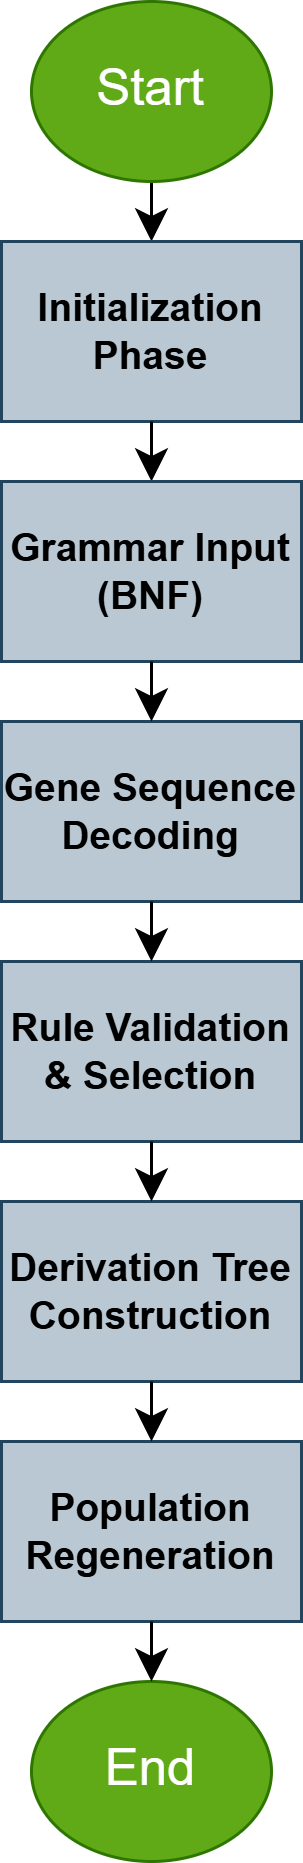
\includegraphics[scale=0.5]{fchart}
\par\end{centering}
\caption{The Grammatical Evolution process used to produce valid programs.\label{fig:geProcess}}
\end{figure}
The BNF grammar for the method of neural network construction is shown
in Figure \ref{fig:nncGrammar}. The numbers shown in parentheses
represent the increasing numbers of the production rules for every
non - terminal symbol. 

\begin{figure}[H]
\begin{lyxcode}
\begin{alignat*}{2}
S & \ ::=\ \langle\text{Sigval}\rangle &  & (0)\\[1ex]
\langle\text{Sigval}\rangle & \ ::=\ \langle\text{Node}\rangle &  & (0)\\
 & \qquad|\,\langle\text{Node}\rangle+\langle\text{Sigval}\rangle &  & (1)\\[1ex]
\langle\text{Node}\rangle & \ ::=\ \langle\text{Number}\rangle*\text{sig}(\langle\text{Sum}\rangle+\langle\text{Number}\rangle) &  & (0)\\[1ex]
\langle\text{Sum}\rangle & \ ::=\ \langle\text{Number}\rangle*\langle\text{Xlist}\rangle &  & (0)\\
 & \qquad|\,\langle\text{Sum}\rangle+\langle\text{Sum}\rangle &  & (1)\\[1ex]
\langle\text{Xlist}\rangle & \ ::=\ x_{1} &  & (0)\\
 & \qquad|\,x_{2} &  & (1)\\
 & \qquad\vdots\\
 & \qquad|\,x_{d} &  & (d-1)\\[1ex]
\langle\text{Number}\rangle & \ ::=\ (\langle\text{Dlist}\rangle.\langle\text{Dlist}\rangle) &  & (0)\\
 & \qquad|\,(-\langle\text{Dlist}\rangle.\langle\text{Dlist}\rangle) &  & (1)\\[1ex]
\langle\text{Dlist}\rangle & \ ::=\ \langle\text{Digit}\rangle &  & (0)\\
 & \qquad|\,\langle\text{Digit}\rangle\langle\text{Dlist}\rangle &  & (1)\\[1ex]
\langle\text{Digit}\rangle & \ ::=\ 0 &  & (0)\\
 & \qquad|\,1 &  & (1)\\
 & \qquad\vdots\\
 & \qquad|\,9 &  & (9)\\
\end{alignat*}
\end{lyxcode}
\caption{The proposed grammar for the construction of artificial neural networks
through Grammatical Evolution.\label{fig:nncGrammar}}
\end{figure}
As an example of produced neural network, consider the following following
form:
\begin{equation}
N(x)=1.9\mbox{sig}\left(10.5x_{1}+3.2x_{3}+1.4\right)+2.1\mbox{sig}\left(2.2x_{2}-3.3x_{3}+3.2\right)
\end{equation}
This neural network stands for a network with 3 inputs $\left(x_{1},x_{2},x_{3}\right)$.
The number of processing units is $H=2$. The network can be shown
graphically in Figure \ref{fig:nnExample}. The above procedure can
produce artificial neural networks with one hidden layer, in which
the number of neurons is not predetermined and is decided dynamically
during the production of the network. In addition, the connections
of the inputs to the neurons are decided dynamically during the construction
of the network and therefore it is not mandatory that all inputs are
connected to every neuron. Finally, the above grammar can be extended
in the future to include artificial neural networks with more than
one processing layer.

\begin{figure}[H]
\begin{centering}
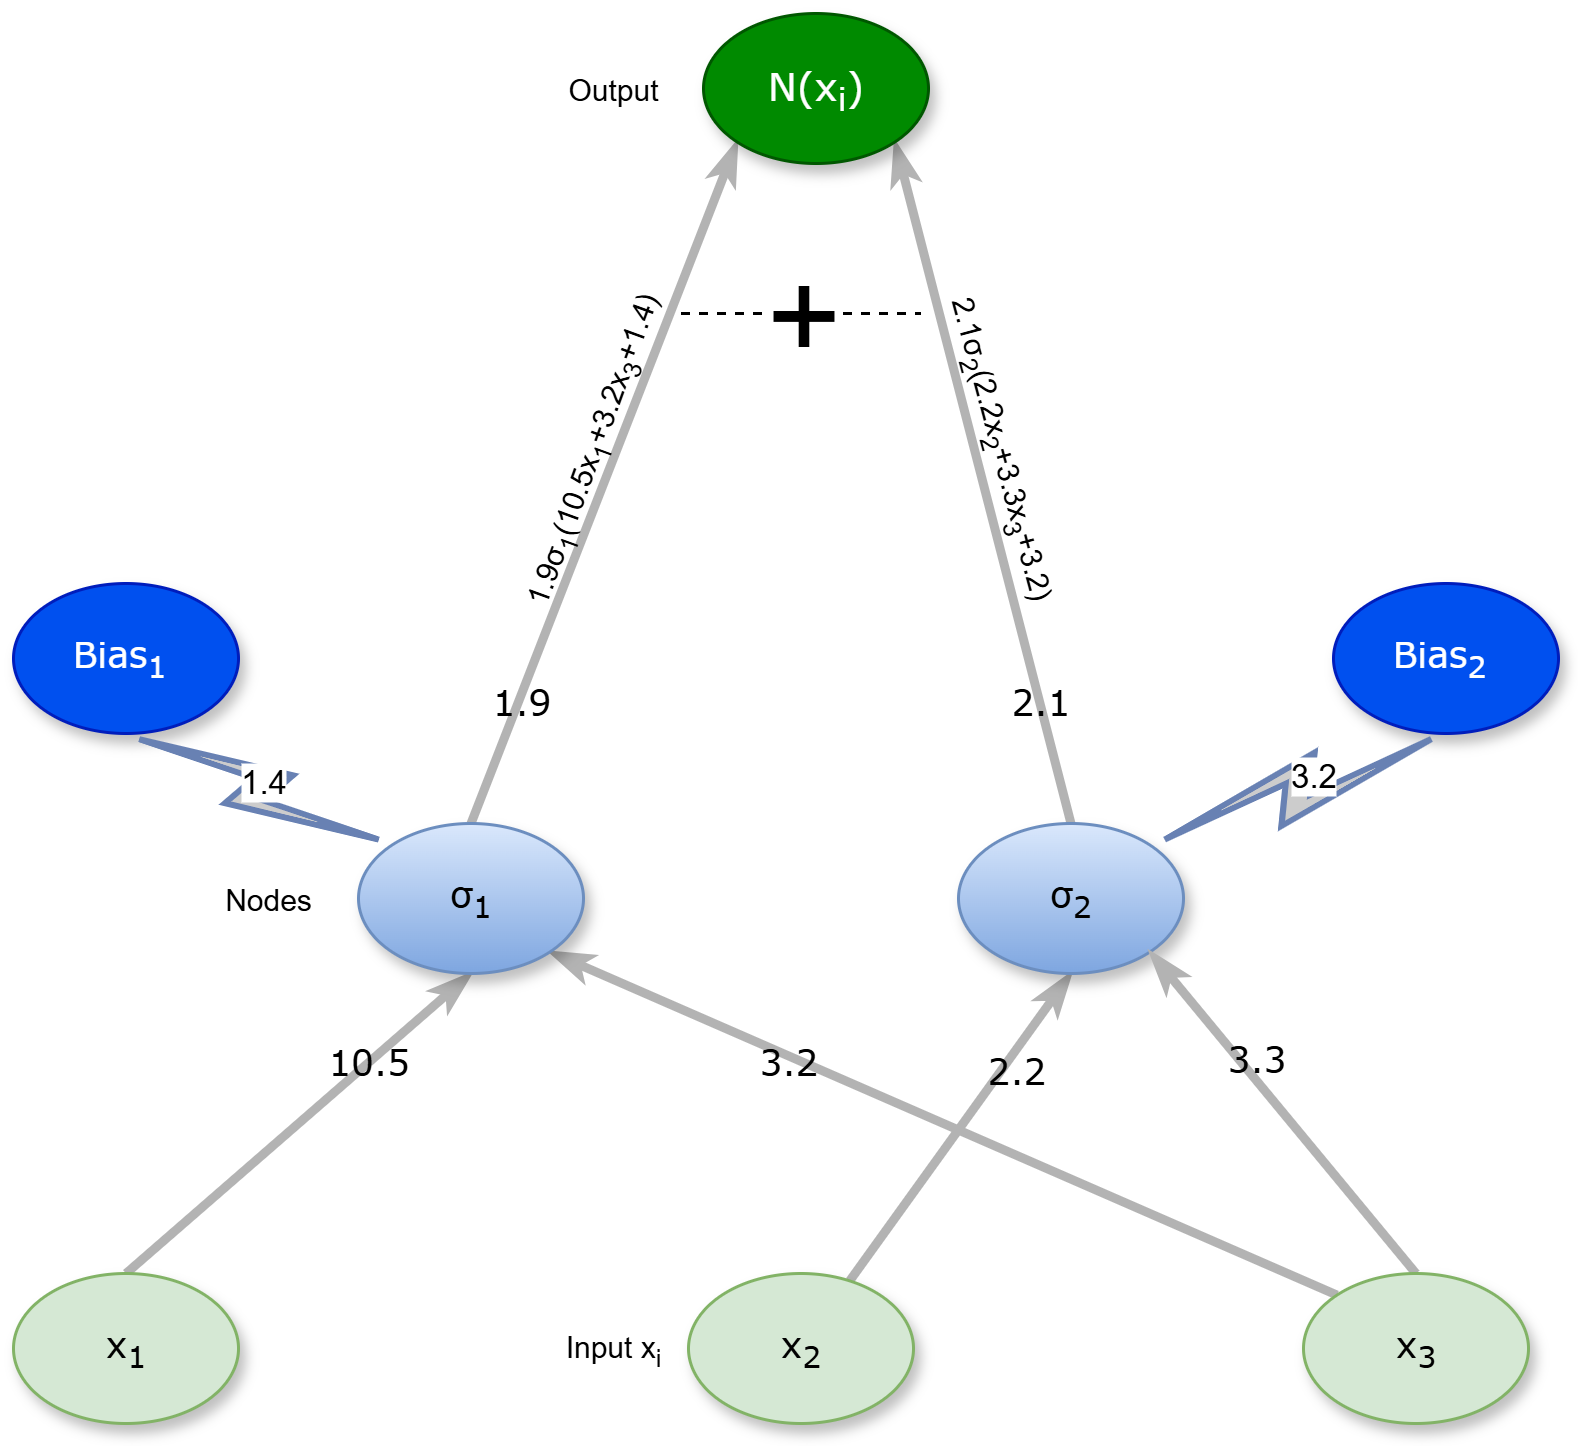
\includegraphics[scale=0.75]{diagram}
\par\end{centering}
\caption{An example of a produced neural network.\label{fig:nnExample}}
\end{figure}
The main steps of the proposed algorithm have as follows:
\begin{enumerate}
\item \textbf{Application of first phase. }
\begin{enumerate}
\item \textbf{Set} $I_{w}$ the number of weights for the first phase.
\item \textbf{Execute} the first phase of the proposed method, described
in subsection \ref{subsec:The-first-phase}.
\item \textbf{Obtain} the chromosome $x^{*}$ of the first phase, with the
lowest fitness value.
\item \textbf{Convert} the chromosome $x^{*}$ to the corresponding integer
chromosome $g^{*}$. This chromosome, with the help of the grammar
of Figure \ref{fig:nncGrammar}, can create the chromosome $x^{*}$.
\end{enumerate}
\item \textbf{Initialization step}. 
\begin{enumerate}
\item \textbf{Define} as $N_{c}$ the number of chromosomes and as $N_{g}$
the number of allowed generations.
\item \textbf{Define} as $p_{s}$ the selection rate and as $p_{m}$ the
mutation rate.
\item \textbf{Initialize} the chromosomes $g_{i},\ i=1,\ldots,N_{c}$ as
sets of positive random integers.
\item \textbf{Insert} the chromosome $g^{*}$ to a random position $r_{i}\in\left[1,N_{c}\right]$
\item \textbf{Set} as $k=0$ the generation counter.
\end{enumerate}
\item \textbf{Fitness Calculation step}.
\begin{enumerate}
\item \textbf{For} $i=1,\ldots,N_{c}$ \textbf{do}
\begin{enumerate}
\item \textbf{Create} the constructed neural network $N_{i}\left(\overrightarrow{x},\overrightarrow{w}\right)$
for the corresponding chromosome $g_{i}$ using the grammar of Figure
\ref{fig:nncGrammar}.
\item \textbf{Calculate} the corresponding fitness value $f_{i}$ as\textbf{
\begin{equation}
f_{i}=\sum_{j=1}^{M}\left(N\left(\overrightarrow{x}_{j},\overrightarrow{w}\right)-y_{j}\right)^{2}\label{eq:eq1-1-1}
\end{equation}
}
\end{enumerate}
\item \textbf{End For}
\end{enumerate}
\item \textbf{Application of genetic operations}.
\begin{enumerate}
\item Application of selection procedure: Initially the chromosomes are
sorted with respect to their fitness values. The first $\left(1-p_{s}\right)\times N_{c}$
of them are transferred without changes to the next generation.\textbf{
}The remaining chromosomes will be substituted by new chromosomes
produced by crossover and mutation.
\item Application of crossover procedure: During crossover, for each pair
of new chromosomes defined as $\left(\tilde{z},\tilde{w}\right)$,
two chromosomes $(z,w)$ are selected from the current population
using tournament selection. The new offsprings are produced using
one - point crossover. A graphical example of the one - point crossover
is outlined in Figure \ref{fig:onepoint}.
\item Application of mutation procedure: For every element of each chromosome
a random number $r\in[0,1]$ is selected. The corresponding element
is altered randomly when $r\le p_{m}$.
\end{enumerate}
\item \textbf{Termination check step}.
\begin{enumerate}
\item \textbf{Set} $k=k+1$
\item \textbf{If} $k<N_{g}$ then go to Fitness Calculation Step else go
to Testing Step.
\end{enumerate}
\item \textbf{Testing step}.
\begin{enumerate}
\item \textbf{Obtain} the best chromosome $g^{*}$ with the lowest fitness
value.
\item \textbf{Create} the corresponding neural network $N^{*}\left(\overrightarrow{x},\overrightarrow{w}\right)$
using the grammar of Figure \ref{fig:nncGrammar}.
\item \textbf{Apply} the neural network $N^{*}\left(\overrightarrow{x},\overrightarrow{w}\right)$
to the test data of the objective problem and report the results.
\end{enumerate}
\end{enumerate}
\begin{figure}[H]
\begin{centering}
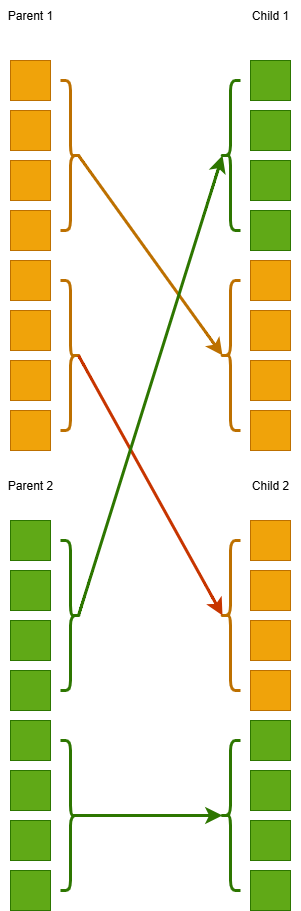
\includegraphics[scale=0.5]{cross2}
\par\end{centering}
\caption{An example of the one - point crossover procedure.\label{fig:onepoint}}

\end{figure}


\section{Results\label{sec:Results}}

The validation of the proposed method was performed with the assistance
of a series of classification and regression datasets, that can be
downloaded freely from the Internet from the following sites:
\begin{enumerate}
\item The UCI database, \url{https://archive.ics.uci.edu/}(accessed on
8 July 2025)\citep{uci}
\item The Keel website, \url{https://sci2s.ugr.es/keel/datasets.php}(accessed
on 8 July 2025)\citep{Keel}.
\item The Statlib URL \url{https://lib.stat.cmu.edu/datasets/index}(accessed
on 8 July 2025). 
\end{enumerate}

\subsection{Experimental datasets}

The following datasets were used in the conducted experiments:
\begin{enumerate}
\item \textbf{Appendictis} which is a medical dataset \citep{appendicitis}. 
\item \textbf{Alcohol}, which is dataset regarding alcohol consumption \citep{alcohol}. 
\item \textbf{Australian}, which is a dataset produced from various bank
transactions \citep{australian}.
\item \textbf{Balance} dataset \citep{balance}, produced from various psychological
experiments.
\item \textbf{Cleveland}, a medical dataset which was discussed in a series
of papers \citep{cleveland1,cleveland2}. 
\item \textbf{Circular} dataset, which is an artificial dataset.
\item \textbf{Dermatology}, a medical dataset for dermatology problems \citep{dermatology}.
\item \textbf{Ecoli}, which is related to protein problems \citep{ecoli}.
\item \textbf{Glass} dataset, that contains measurements from glass component
analysis. 
\item \textbf{Haberman}, a medical dataset related to breast cancer.
\item \textbf{Hayes-roth} dataset \citep{hayes-roth}.
\item \textbf{Heart}, which is a dataset related to heart diseases \citep{heart}.
\item \textbf{HeartAttack}, which is a medical dataset for the detection
of heart diseases
\item \textbf{Housevotes}, a dataset which is related to the Congressional
voting in USA \citep{housevotes}.
\item \textbf{Ionosphere}, a dataset that contains measurements from the
ionosphere \citep{ion1,ion2}.
\item \textbf{Liverdisorder}, a medical dataset that was studied thoroughly
in a series of papers\citep{liver,liver1}.
\item \textbf{Lymography} \citep{lymography}.
\item \textbf{Mammographic}, which is a medical dataset used for the prediction
of breast cancer \citep{mammographic}.
\item \textbf{Parkinsons}, which is a medical dataset used for the detection
of Parkinson's disease \citep{parkinsons1,parkinsons2}.
\item \textbf{Pima}, which is a medical dataset for the detection of diabetes\citep{pima}.
\item \textbf{Phoneme}, a dataset that contains sound measurements.
\item \textbf{Popfailures}, a dataset related to experiments regarding climate
\citep{popfailures}.
\item \textbf{Regions2}, a medical dataset applied to liver problems \citep{regions2}.
\item \textbf{Saheart}, which is a medical dataset concerning heart diseases\citep{saheart}.
\item \textbf{Segment} dataset \citep{segment}.
\item \textbf{Statheart}, a medical dataset related to heart diseases.
\item \textbf{Spiral}, an artificial dataset with two classes.
\item \textbf{Student}, which is a dataset regarding experiments in schools
\citep{student}.
\item \textbf{Transfusion}, which is a medical dataset \citep{transfusion}.
\item \textbf{Wdbc}, which is a medical dataset regarding breast cancer
\citep{wdbc1,wdbc2}.
\item \textbf{Wine}, a dataset regarding measurements about the quality
of wines \citep{wine1,wine2}.
\item \textbf{EEG}, which is dataset regarding EEG recordings \citep{eeg1,eeg2}.
From this dataset the following cases were used: Z\_F\_S, ZO\_NF\_S,
ZONF\_S and Z\_O\_N\_F\_S.
\item \textbf{Zoo}, which is a dataset regarding animal classification \citep{zoo}
.
\end{enumerate}
Moreover a series of regression datasets was adopted in the conducted
experiments. The list with the regression datasets has as follows:
\begin{enumerate}
\item \textbf{Abalone}, which is a dataset about the age of abalones \citep{abalone}.
\item \textbf{Airfoil}, a dataset founded in NASA \citep{airfoil}.
\item \textbf{Auto}, a dataset related to the consumption of fuels from
cars.
\item \textbf{BK}, which is used to predict the points scored in basketball
games. 
\item \textbf{BL}, a dataset that contains measurements from electricity
experiments.
\item \textbf{Baseball}, which is a dataset used to predict the income of
baseball players.
\item \textbf{Concrete}, which is a civil engineering dataset \citep{concrete}.
\item \textbf{DEE}, a dataset that is used to predict the price of electricity.
\item \textbf{Friedman}, which is an artificial dataset\citep{friedman}.
\item \textbf{FY, }which is a dataset regarding the longevity of fruit flies. 
\item \textbf{HO}, a dataset located in the STATLIB repository.
\item \textbf{Housing}, regarding the price of houses \citep{housing}.
\item \textbf{Laser}, which contains measurements from various physics experiments.
\item \textbf{LW}, a dataset regarding the weight of babes.
\item \textbf{Mortgage}, a dataset that contains measurements from the economy
of USA.
\item \textbf{PL} dataset, located in the STALIB repository.
\item \textbf{Plastic}, a dataset regarding problems occurred with the pressure
on plastics.
\item \textbf{Quake}, a dataset regarding the measurements of earthquakes.
\item \textbf{SN}, a dataset related to trellising and pruning.
\item \textbf{Stock}, which is a dataset regarding stocks.
\item \textbf{Treasury}, a dataset that contains measurements from the economy
of USA.
\end{enumerate}

\subsection{Experiments}

The software used in the experiment was coded in C++ with the assistance
of the freely available Optimus environment \citep{optimus}. The
experiments were conducted 30 times, using different seed for the
random generator each time. The validation of the experiments was
performed using the method of ten - fold cross validation. The average
classification error as calculated on the test is reported for the
classification datasets and the average regression error for the regression
datasets. The classification error is computed using the following
formula:
\begin{equation}
E_{C}\left(N\left(\overrightarrow{x},\overrightarrow{w}\right)\right)=100\times\frac{\sum_{i=1}^{N}\left(\mbox{class}\left(N\left(\overrightarrow{x_{i}},\overrightarrow{w}\right)\right)-y_{i}\right)}{N}
\end{equation}
For the calculation of this error, the test set $T$ is a set $T=\left(x_{i},y_{i}\right),\ i=1,\ldots,N$
is used. Similarly, the average regression error is reported for the
regression datasets and it is calculated as follows:
\begin{equation}
E_{R}\left(N\left(\overrightarrow{x},\overrightarrow{w}\right)\right)=\frac{\sum_{i=1}^{N}\left(N\left(\overrightarrow{x_{i}},\overrightarrow{w}\right)-y_{i}\right)^{2}}{N}
\end{equation}
The experimental settings are shown in Table \ref{tab:expValues}.
The parameter values have been set so that there is a compromise between
the efficiency and speed of the methodologies used when performing
the experiments. In the following tables that describe the experimental
results the following notation is used:
\begin{enumerate}
\item The column DATASET stands for the used dataset.
\item The column ADAM denotes the usage of the ADAM optimization method
\citep{nn_adam} in order to train a neural network with $H=10$ processing
nodes.
\item The column BFGS stands for the incorporation of a BFGS variant of
Powell \citep{powell} for the training of an artificial neural network
with $H=10$ processing nodes.
\item The column GENETIC denotes the usage of a Genetic Algorithm with the
same parameter set as provided in Table \ref{tab:expValues} to train
a neural network with $H=10$ processing nodes.
\item The column RBF describes the incorporation of a Radial Basis Function
(RBF) network \citep{rbf1,rbf2} with $H=10$ hidden nodes.
\item The column NNC stands for the usage of the original neural construction
method.
\item The column NEAT represents the usage of the NEAT method (NeuroEvolution
of Augmenting Topologies ) \citep{neat}.
\item The column PRUNE stands for the the usage of OBS pruning method \citep{prune},
provided by Fast Compressed Neural Networks library \citep{fcn}.
\item The column PROPOSED denotes the usage of the proposed method.
\item The row AVERAGE represents the average classification or regression
error for all datasets in the corresponding table.
\end{enumerate}
\begin{table}[H]
\caption{The values for the parameters of the proposed method.\label{tab:expValues}}

\centering{}%
\begin{tabular}{|c|c|c|}
\hline 
PARAMETER & MEANING & VALUE\tabularnewline
\hline 
\hline 
$N_{c}$ & Chromosomes & 500\tabularnewline
\hline 
$N_{g}$ & Maximum number of generations & 500\tabularnewline
\hline 
$p_{s}$ & Selection rate & 0.1\tabularnewline
\hline 
$p_{m}$ & Mutation rate & 0.05\tabularnewline
\hline 
$I_{w}$ & Number of weights for the first phase & 10\tabularnewline
\hline 
\end{tabular}
\end{table}

In Table \ref{tab:expClass}, classification error rates are presented
for a variety of machine learning models applied to different classification
datasets. Each row in the table corresponds to a specific dataset,
while the columns represent individual methods: ADAM, BFGS, GENETIC,
RBF, NEAT, PRUNE, NNC, and PROPOSED. The values indicate error percentages,
meaning that lower values correspond to better model performance on
each dataset. The final row shows the average error rate for each
model, serving as a general indicator of overall performance across
all datasets. Based on the analysis of the average errors, it becomes
evident that the PROPOSED method achieves the lowest average error
rate, with a value of 19.63\%. This suggests that it generally outperforms
the other methods. It is followed by the NNC model with an average
error of 24.79\%, which also demonstrates a significantly lower error
compared to traditional approaches such as ADAM, BFGS, and GENETIC,
whose average error rates are 36.45\%, 35.71\%, and 28.25\% respectively.
The PRUNE method also performs relatively well, with a mean error
of 27.94\%. On an individual dataset level, the PROPOSED method achieves
the best performance (i.e., the lowest error) in a considerable number
of cases, such as in the CIRCULAR, DERMATOLOGY, SEGMENT, Z\_F\_S,
ZO\_NF\_S, ZONF\_S, and ZOO datasets, where it records the smallest
error among all methods. Furthermore, in many of these cases, the
performance gap between the PROPOSED method and the others is quite
significant, indicating the method's stability and reliability across
various data conditions and structures. Some models, including GENETIC,
RBF, and NEAT, tend to show relatively high errors in several datasets,
which may be due to issues such as overfitting, poor adaptation to
non-linear relationships, or generally weaker generalization capabilities.
In contrast, the NNC and PRUNE models demonstrate more consistent
behavior, while the PROPOSED method maintains not only the lowest
overall error but also reliable performance across a wide range of
problem types. In summary, the statistical analysis of classification
error rates confirms the superiority of the PROPOSED method over the
others, both in terms of average performance and the number of datasets
in which it excels. This conclusion is further supported by the observation
that the PROPOSED method achieves the best results in the majority
of datasets, often with significantly lower error rates. Such superiority
may be attributed to better adaptability to data characteristics,
effective avoidance of overfitting, and, more broadly, a more flexible
or advanced algorithmic architecture.

\begin{table}[H]
\caption{Experimental results using a variety of machine learning methods for
the classification datasets.\label{tab:expClass}}

\centering{}{\footnotesize{}%
\begin{tabular}{|c|c|c|c|c|c|c|c|c|}
\hline 
{\footnotesize DATASET} & {\footnotesize ADAM} & {\footnotesize BFGS} & {\footnotesize GENETIC} & {\footnotesize RBF} & {\footnotesize NEAT} & {\footnotesize PRUNE} & {\footnotesize NNC} & {\footnotesize PROPOSED}\tabularnewline
\hline 
\hline 
{\footnotesize APPENDICITIS} & {\footnotesize 16.50\%} & {\footnotesize 18.00\%} & {\footnotesize 24.40\%} & {\footnotesize 12.23\%} & {\footnotesize 17.20\%} & {\footnotesize 15.97\%} & {\footnotesize 14.40\%} & {\footnotesize 16.30\%}\tabularnewline
\hline 
{\footnotesize ALCOHOL} & {\footnotesize 57.78\%} & {\footnotesize 41.50\%} & {\footnotesize 39.57\%} & {\footnotesize 49.32\%} & {\footnotesize 66.80\%} & {\footnotesize 15.75\%} & {\footnotesize 37.72\%} & {\footnotesize 20.21\%}\tabularnewline
\hline 
{\footnotesize AUSTRALIAN} & {\footnotesize 35.65\%} & {\footnotesize 38.13\%} & {\footnotesize 32.21\%} & {\footnotesize 34.89\%} & {\footnotesize 31.98\%} & {\footnotesize 43.66\%} & {\footnotesize 14.46\%} & {\footnotesize 14.68\%}\tabularnewline
\hline 
{\footnotesize BALANCE} & {\footnotesize 12.27\%} & {\footnotesize 8.64\%} & {\footnotesize 8.97\%} & {\footnotesize 33.53\%} & {\footnotesize 23.14\%} & {\footnotesize 9.00\%} & {\footnotesize 23.65\%} & {\footnotesize 7.26\%}\tabularnewline
\hline 
{\footnotesize CLEVELAND} & {\footnotesize 67.55\%} & {\footnotesize 77.55\%} & {\footnotesize 51.60\%} & {\footnotesize 67.10\%} & {\footnotesize 53.44\%} & {\footnotesize 51.48\%} & {\footnotesize 50.93\%} & {\footnotesize 44.90\%}\tabularnewline
\hline 
{\footnotesize CIRCULAR} & {\footnotesize 19.95\%} & {\footnotesize 6.08\%} & {\footnotesize 5.99\%} & {\footnotesize 5.98\%} & {\footnotesize 35.18\%} & {\footnotesize 12.76\%} & {\footnotesize 12.66\%} & {\footnotesize 4.22\%}\tabularnewline
\hline 
{\footnotesize DERMATOLOGY} & {\footnotesize 26.14\%} & {\footnotesize 52.92\%} & {\footnotesize 30.58\%} & {\footnotesize 62.34\%} & {\footnotesize 32.43\%} & {\footnotesize 9.02\%} & {\footnotesize 21.54\%} & {\footnotesize 5.92\%}\tabularnewline
\hline 
{\footnotesize ECOLI} & {\footnotesize 64.43\%} & {\footnotesize 69.52\%} & {\footnotesize 54.67\%} & {\footnotesize 59.48\%} & {\footnotesize 43.44\%} & {\footnotesize 60.32\%} & {\footnotesize 49.88\%} & {\footnotesize 44.79\%}\tabularnewline
\hline 
{\footnotesize GLASS} & {\footnotesize 61.38\%} & {\footnotesize 54.67\%} & {\footnotesize 52.86\%} & {\footnotesize 50.46\%} & {\footnotesize 55.71\%} & {\footnotesize 66.19\%} & {\footnotesize 56.09\%} & {\footnotesize 49.43\%}\tabularnewline
\hline 
{\footnotesize HABERMAN} & {\footnotesize 29.00\%} & {\footnotesize 29.34\%} & {\footnotesize 28.66\%} & {\footnotesize 25.10\%} & {\footnotesize 24.04\%} & {\footnotesize 29.38\%} & {\footnotesize 27.53\%} & {\footnotesize 28.57\%}\tabularnewline
\hline 
{\footnotesize HAYES-ROTH} & {\footnotesize 59.70\%} & {\footnotesize 37.33\%} & {\footnotesize 56.18\%} & {\footnotesize 64.36\%} & {\footnotesize 50.15\%} & {\footnotesize 45.44\%} & {\footnotesize 33.69\%} & {\footnotesize 30.77\%}\tabularnewline
\hline 
{\footnotesize HEART} & {\footnotesize 38.53\%} & {\footnotesize 39.44\%} & {\footnotesize 28.34\%} & {\footnotesize 31.20\%} & {\footnotesize 39.27\%} & {\footnotesize 27.21\%} & {\footnotesize 15.67\%} & {\footnotesize 17.85\%}\tabularnewline
\hline 
{\footnotesize HEARTATTACK} & {\footnotesize 45.55\%} & {\footnotesize 46.67\%} & {\footnotesize 29.03\%} & {\footnotesize 29.00\%} & {\footnotesize 32.34\%} & {\footnotesize 29.26\%} & {\footnotesize 20.87\%} & {\footnotesize 20.67\%}\tabularnewline
\hline 
{\footnotesize HOUSEVOTES} & {\footnotesize 7.48\%} & {\footnotesize 7.13\%} & {\footnotesize 6.62\%} & {\footnotesize 6.13\%} & {\footnotesize 10.89\%} & {\footnotesize 5.81\%} & {\footnotesize 3.17\%} & {\footnotesize 7.39\%}\tabularnewline
\hline 
{\footnotesize IONOSPHERE} & {\footnotesize 16.64\%} & {\footnotesize 15.29\%} & {\footnotesize 15.14\%} & {\footnotesize 16.22\%} & {\footnotesize 19.67\%} & {\footnotesize 11.32\%} & {\footnotesize 11.29\%} & {\footnotesize 13.14\%}\tabularnewline
\hline 
{\footnotesize LIVERDISORDER} & {\footnotesize 41.53\%} & {\footnotesize 42.59\%} & {\footnotesize 31.11\%} & {\footnotesize 30.84\%} & {\footnotesize 30.67\%} & {\footnotesize 49.72\%} & {\footnotesize 32.35\%} & {\footnotesize 33.38\%}\tabularnewline
\hline 
{\footnotesize LYMOGRAPHY} & {\footnotesize 39.79\%} & {\footnotesize 35.43\%} & {\footnotesize 28.42\%} & {\footnotesize 25.50\%} & {\footnotesize 33.70\%} & {\footnotesize 22.02\%} & {\footnotesize 25.29\%} & {\footnotesize 25.14\%}\tabularnewline
\hline 
{\footnotesize MAMMOGRAPHIC} & {\footnotesize 46.25\%} & {\footnotesize 17.24\%} & {\footnotesize 19.88\%} & {\footnotesize 21.38\%} & {\footnotesize 22.85\%} & {\footnotesize 38.10\%} & {\footnotesize 17.62\%} & {\footnotesize 17.77\%}\tabularnewline
\hline 
{\footnotesize PARKINSONS} & {\footnotesize 24.06\%} & {\footnotesize 27.58\%} & {\footnotesize 18.05\%} & {\footnotesize 17.41\%} & {\footnotesize 18.56\%} & {\footnotesize 22.12\%} & {\footnotesize 12.74\%} & {\footnotesize 14.05\%}\tabularnewline
\hline 
{\footnotesize PIMA} & {\footnotesize 34.85\%} & {\footnotesize 35.59\%} & {\footnotesize 32.19\%} & {\footnotesize 25.78\%} & {\footnotesize 34.51\%} & {\footnotesize 35.08\%} & {\footnotesize 28.07\%} & {\footnotesize 24.34\%}\tabularnewline
\hline 
{\footnotesize POPFAILURES} & {\footnotesize 5.18\%} & {\footnotesize 5.24\%} & {\footnotesize 5.94\%} & {\footnotesize 7.04\%} & {\footnotesize 7.05\%} & {\footnotesize 4.79\%} & {\footnotesize 6.98\%} & {\footnotesize 7.19\%}\tabularnewline
\hline 
{\footnotesize REGIONS2} & {\footnotesize 29.85\%} & {\footnotesize 36.28\%} & {\footnotesize 29.39\%} & {\footnotesize 38.29\%} & {\footnotesize 33.23\%} & {\footnotesize 34.26\%} & {\footnotesize 26.18\%} & {\footnotesize 25.00\%}\tabularnewline
\hline 
{\footnotesize SAHEART} & {\footnotesize 34.04\%} & {\footnotesize 37.48\%} & {\footnotesize 34.86\%} & {\footnotesize 32.19\%} & {\footnotesize 34.51\%} & {\footnotesize 37.70\%} & {\footnotesize 29.80\%} & {\footnotesize 30.11\%}\tabularnewline
\hline 
{\footnotesize SEGMENT} & {\footnotesize 49.75\%} & {\footnotesize 68.97\%} & {\footnotesize 57.72\%} & {\footnotesize 59.68\%} & {\footnotesize 66.72\%} & {\footnotesize 60.40\%} & {\footnotesize 53.50\%} & {\footnotesize 9.59\%}\tabularnewline
\hline 
{\footnotesize SPIRAL} & {\footnotesize 47.67\%} & {\footnotesize 47.99\%} & {\footnotesize 48.66\%} & {\footnotesize 44.87\%} & {\footnotesize 48.66\%} & {\footnotesize 50.38\%} & {\footnotesize 48.01\%} & {\footnotesize 41.25\%}\tabularnewline
\hline 
{\footnotesize STATHEART} & {\footnotesize 44.04\%} & {\footnotesize 39.65\%} & {\footnotesize 27.25\%} & {\footnotesize 31.36\%} & {\footnotesize 44.36\%} & {\footnotesize 28.37\%} & {\footnotesize 18.08\%} & {\footnotesize 20.26\%}\tabularnewline
\hline 
{\footnotesize STUDENT} & {\footnotesize 5.13\%} & {\footnotesize 7.14\%} & {\footnotesize 5.61\%} & {\footnotesize 5.49\%} & {\footnotesize 10.20\%} & {\footnotesize 10.84\%} & {\footnotesize 6.70\%} & {\footnotesize 7.18\%}\tabularnewline
\hline 
{\footnotesize TRANSFUSION} & {\footnotesize 25.68\%} & {\footnotesize 25.84\%} & {\footnotesize 24.87\%} & {\footnotesize 26.41\%} & {\footnotesize 24.87\%} & {\footnotesize 29.35\%} & {\footnotesize 25.77\%} & {\footnotesize 23.59\%}\tabularnewline
\hline 
{\footnotesize WDBC} & {\footnotesize 35.35\%} & {\footnotesize 29.91\%} & {\footnotesize 8.56\%} & {\footnotesize 7.27\%} & {\footnotesize 12.88\%} & {\footnotesize 15.48\%} & {\footnotesize 7.36\%} & {\footnotesize 3.73\%}\tabularnewline
\hline 
{\footnotesize WINE} & {\footnotesize 29.40\%} & {\footnotesize 59.71\%} & {\footnotesize 19.20\%} & {\footnotesize 31.41\%} & {\footnotesize 25.43\%} & {\footnotesize 16.62\%} & {\footnotesize 13.59\%} & {\footnotesize 10.41\%}\tabularnewline
\hline 
{\footnotesize Z\_F\_S} & {\footnotesize 47.81\%} & {\footnotesize 39.37\%} & {\footnotesize 10.73\%} & {\footnotesize 13.16\%} & {\footnotesize 38.41\%} & {\footnotesize 17.91\%} & {\footnotesize 14.53\%} & {\footnotesize 6.60\%}\tabularnewline
\hline 
{\footnotesize Z\_O\_N\_F\_S} & {\footnotesize 78.79\%} & {\footnotesize 65.67\%} & {\footnotesize 64.81\%} & {\footnotesize 48.70\%} & {\footnotesize 77.08\%} & {\footnotesize 71.29\%} & {\footnotesize 48.62\%} & {\footnotesize 49.66\%}\tabularnewline
\hline 
{\footnotesize ZO\_NF\_S} & {\footnotesize 47.43\%} & {\footnotesize 43.04\%} & {\footnotesize 21.54\%} & {\footnotesize 9.02\%} & {\footnotesize 43.75\%} & {\footnotesize 15.57\%} & {\footnotesize 13.54\%} & {\footnotesize 3.94\%}\tabularnewline
\hline 
{\footnotesize ZONF\_S} & {\footnotesize 11.99\%} & {\footnotesize 15.62\%} & {\footnotesize 4.36\%} & {\footnotesize 4.03\%} & {\footnotesize 5.44\%} & {\footnotesize 3.27\%} & {\footnotesize 2.64\%} & {\footnotesize 2.60\%}\tabularnewline
\hline 
{\footnotesize ZOO} & {\footnotesize 14.13\%} & {\footnotesize 10.70\%} & {\footnotesize 9.50\%} & {\footnotesize 21.93\%} & {\footnotesize 20.27\%} & {\footnotesize 8.53\%} & {\footnotesize 8.70\%} & {\footnotesize 5.10\%}\tabularnewline
\hline 
{\footnotesize\textbf{AVERAGE}} & {\footnotesize\textbf{35.75\%}} & {\footnotesize\textbf{35.24\%}} & {\footnotesize\textbf{27.64\%}} & {\footnotesize\textbf{29.97\%}} & {\footnotesize\textbf{33.40\%}} & {\footnotesize\textbf{28.70\%}} & {\footnotesize\textbf{23.82\%}} & {\footnotesize\textbf{19.63\%}}\tabularnewline
\hline 
\end{tabular}}{\footnotesize\par}
\end{table}
Table \ref{tab:expRegression} presents the performance of various
machine learning methods on regression datasets. In this table, columns
represent different algorithms, and rows correspond to datasets. The
numerical values shown are absolute errors, indicating the magnitude
of deviation from the actual values. Therefore, smaller values signify
higher prediction accuracy for the corresponding model. The last row
reports the average error for each method across all datasets, offering
a general measure of overall performance. According to the overall
results, the PROPOSED method exhibits the lowest average error value
at 4.83, indicating high accuracy and better overall behavior compared
to the other approaches. The second-best performing model is NNC,
with an average error of 6.29, which also stands out from the traditional
methods. On the other hand, ADAM and BFGS show significantly higher
error rates, at 22.46 and 30.29 respectively, suggesting that these
methods may not adapt well to the specific characteristics of the
regression problems evaluated. At the individual dataset level, the
PROPOSED method achieves notably low error values across multiple
datasets, including AIRFOIL, CONCRETE, LASER, PL, PLASTIC, and STOCK,
outperforming other algorithms by a considerable margin. Its consistent
performance across such diverse problems suggests that it is a flexible
and reliable approach. Furthermore, the fact that it also performs
strongly on more complex datasets with high variability in error---such
as AUTO and BASEBALL---strengthens the impression that the method
adapts effectively to varying data structures. By comparison, algorithms
such as GENETIC and RBF exhibit less stable behavior, showing good
performance in some datasets but poor results in others, resulting
in a higher overall average error. The PRUNE method, although not
a traditional algorithm, shows moderate performance overall, while
NEAT does not appear to stand out in any particular dataset and also
maintains a relatively high average error. In conclusion, the analysis
indicates that the PROPOSED method clearly excels in predictive accuracy,
both on average and across a large number of individual datasets.
Its ability to minimize error across different types of problems makes
it a particularly promising option for regression tasks involving
heterogeneous data.

\begin{table}[H]
\caption{Experimental results using a variety of machine learning methods on
the regression datasets.\label{tab:expRegression}}

\centering{}{\footnotesize{}%
\begin{tabular}{|c|c|c|c|c|c|c|c|c|}
\hline 
{\footnotesize DATASET} & {\footnotesize ADAM} & {\footnotesize BFGS} & {\footnotesize GENETIC} & {\footnotesize RBF} & {\footnotesize NEAT} & {\footnotesize PRUNE} & {\footnotesize NNC} & {\footnotesize PROPOSED}\tabularnewline
\hline 
\hline 
{\footnotesize ABALONE} & {\footnotesize 4.30} & {\footnotesize 5.69} & {\footnotesize 7.17} & {\footnotesize 7.37} & {\footnotesize 9.88} & {\footnotesize 7.88} & {\footnotesize 5.08} & {\footnotesize 4.41}\tabularnewline
\hline 
{\footnotesize AIRFOIL} & {\footnotesize 0.005} & {\footnotesize 0.003} & {\footnotesize 0.003} & {\footnotesize 0.27} & {\footnotesize 0.067} & {\footnotesize 0.002} & {\footnotesize 0.004} & {\footnotesize 0.001}\tabularnewline
\hline 
{\footnotesize AUTO} & {\footnotesize 70.84} & {\footnotesize 60.97} & {\footnotesize 12.18} & {\footnotesize 17.87} & {\footnotesize 56.06} & {\footnotesize 75.59} & {\footnotesize 17.13} & {\footnotesize 11.73}\tabularnewline
\hline 
{\footnotesize BK} & {\footnotesize 0.0252} & {\footnotesize 0.28} & {\footnotesize 0.027} & {\footnotesize 0.02} & {\footnotesize 0.15} & {\footnotesize 0.027} & {\footnotesize 0.10} & {\footnotesize 0.058}\tabularnewline
\hline 
{\footnotesize BL} & {\footnotesize 0.622} & {\footnotesize 2.55} & {\footnotesize 5.74} & {\footnotesize 0.013} & {\footnotesize 0.05} & {\footnotesize 0.027} & {\footnotesize 1.19} & {\footnotesize 0.13}\tabularnewline
\hline 
{\footnotesize BASEBALL} & {\footnotesize 77.90} & {\footnotesize 119.63} & {\footnotesize 103.60} & {\footnotesize 93.02} & {\footnotesize 100.39} & {\footnotesize 94.50} & {\footnotesize 61.57} & {\footnotesize 60.42}\tabularnewline
\hline 
{\footnotesize CONCRETE} & {\footnotesize 0.078} & {\footnotesize 0.066} & {\footnotesize 0.0099} & {\footnotesize 0.011} & {\footnotesize 0.081} & {\footnotesize 0.0077} & {\footnotesize 0.008} & {\footnotesize 0.004}\tabularnewline
\hline 
{\footnotesize DEE} & {\footnotesize 0.63} & {\footnotesize 2.36} & {\footnotesize 1.013} & {\footnotesize 0.17} & {\footnotesize 1.512} & {\footnotesize 1.08} & {\footnotesize 0.26} & {\footnotesize 0.26}\tabularnewline
\hline 
{\footnotesize FRIEDMAN} & {\footnotesize 22.90} & {\footnotesize 1.263} & {\footnotesize 1.249} & {\footnotesize 7.23} & {\footnotesize 19.35} & {\footnotesize 8.69} & {\footnotesize 6.29} & {\footnotesize 1.25}\tabularnewline
\hline 
{\footnotesize FY} & {\footnotesize 0.038} & {\footnotesize 0.19} & {\footnotesize 0.65} & {\footnotesize 0.041} & {\footnotesize 0.08} & {\footnotesize 0.042} & {\footnotesize 0.11} & {\footnotesize 0.13}\tabularnewline
\hline 
{\footnotesize HO} & {\footnotesize 0.035} & {\footnotesize 0.62} & {\footnotesize 2.78} & {\footnotesize 0.03} & {\footnotesize 0.169} & {\footnotesize 0.03} & {\footnotesize 0.015} & {\footnotesize 0.073}\tabularnewline
\hline 
{\footnotesize HOUSING} & {\footnotesize 80.99} & {\footnotesize 97.38} & {\footnotesize 43.26} & {\footnotesize 57.68} & {\footnotesize 56.49} & {\footnotesize 52.25} & {\footnotesize 25.47} & {\footnotesize 15.96}\tabularnewline
\hline 
{\footnotesize LASER} & {\footnotesize 0.03} & {\footnotesize 0.015} & {\footnotesize 0.59} & {\footnotesize 0.03} & {\footnotesize 0.084} & {\footnotesize 0.007} & {\footnotesize 0.025} & {\footnotesize 0.004}\tabularnewline
\hline 
{\footnotesize LW} & {\footnotesize 0.028} & {\footnotesize 2.98} & {\footnotesize 1.90} & {\footnotesize 0.03} & {\footnotesize 0.03} & {\footnotesize 0.02} & {\footnotesize 0.011} & {\footnotesize 0.32}\tabularnewline
\hline 
{\footnotesize MORTGAGE} & {\footnotesize 9.24} & {\footnotesize 8.23} & {\footnotesize 2.41} & {\footnotesize 1.45} & {\footnotesize 14.11} & {\footnotesize 12.96} & {\footnotesize 0.30} & {\footnotesize 0.15}\tabularnewline
\hline 
{\footnotesize PL} & {\footnotesize 0.117} & {\footnotesize 0.29} & {\footnotesize 0.29} & {\footnotesize 2.118} & {\footnotesize 0.09} & {\footnotesize 0.032} & {\footnotesize 0.047} & {\footnotesize 0.021}\tabularnewline
\hline 
{\footnotesize PLASTIC} & {\footnotesize 11.71} & {\footnotesize 20.32} & {\footnotesize 2.791} & {\footnotesize 8.62} & {\footnotesize 20.77} & {\footnotesize 17.33} & {\footnotesize 4.20} & {\footnotesize 2.15}\tabularnewline
\hline 
{\footnotesize QUAKE} & {\footnotesize 0.07} & {\footnotesize 0.42} & {\footnotesize 0.04} & {\footnotesize 0.07} & {\footnotesize 0.298} & {\footnotesize 0.04} & {\footnotesize 0.96} & {\footnotesize 0.061}\tabularnewline
\hline 
{\footnotesize SN} & {\footnotesize 0.026} & {\footnotesize 0.40} & {\footnotesize 2.95} & {\footnotesize 0.027} & {\footnotesize 0.174} & {\footnotesize 0.032} & {\footnotesize 0.026} & {\footnotesize 0.10}\tabularnewline
\hline 
{\footnotesize STOCK} & {\footnotesize 180.89} & {\footnotesize 302.43} & {\footnotesize 3.88} & {\footnotesize 12.23} & {\footnotesize 12.23} & {\footnotesize 39.08} & {\footnotesize 8.92} & {\footnotesize 3.96}\tabularnewline
\hline 
{\footnotesize TREASURY} & {\footnotesize 11.16} & {\footnotesize 9.91} & {\footnotesize 2.93} & {\footnotesize 2.02} & {\footnotesize 15.52} & {\footnotesize 13.76} & {\footnotesize 0.43} & {\footnotesize 0.25}\tabularnewline
\hline 
{\footnotesize\textbf{AVERAGE}} & {\footnotesize\textbf{22.46}} & {\footnotesize\textbf{30.29}} & {\footnotesize\textbf{9.31}} & {\footnotesize\textbf{10.02}} & {\footnotesize\textbf{14.65}} & {\footnotesize\textbf{15.40}} & {\footnotesize\textbf{6.29}} & {\footnotesize\textbf{4.83}}\tabularnewline
\hline 
\end{tabular}}{\footnotesize\par}
\end{table}
To determine the significance levels of the experimental results presented
in the classification dataset tables, statistical analyses were conducted.
Exclusively, the non-parametric, paired Wilcoxon signed-rank test
was used to assess the statistical significance of the differences
between the proposed method and the other methods, as well as for
hyperparameter comparisons in both classification and regression tasks.
These analyses were based on the critical parameter \textquotedbl p\textquotedbl ,
which is used to assess the statistical significance of performance
differences between models. As shown in Figure \ref{fig:statClass},
the differences in performance between the PROPOSED model and all
other models namely ADAM, BFGS, GENETIC, RBF, NEAT, and PRUNE are
extremely statistically significant with p \textless{} 0.0001. This
indicates, with a high level of confidence, that the PROPOSED model
outperforms the rest in classification accuracy. Even the comparison
with NNC, which is the model with the closest average performance,
showed a statistically significant difference with p \textless{} 0.05.
This confirms that the superiority of the PROPOSED model is not due
to random variation but is statistically sound and consistent. Therefore,
the PROPOSED model can be confidently considered the best choice among
the evaluated models for classification tasks, based on the experimental
data and corresponding statistical analysis.

\begin{figure}[H]
\begin{centering}
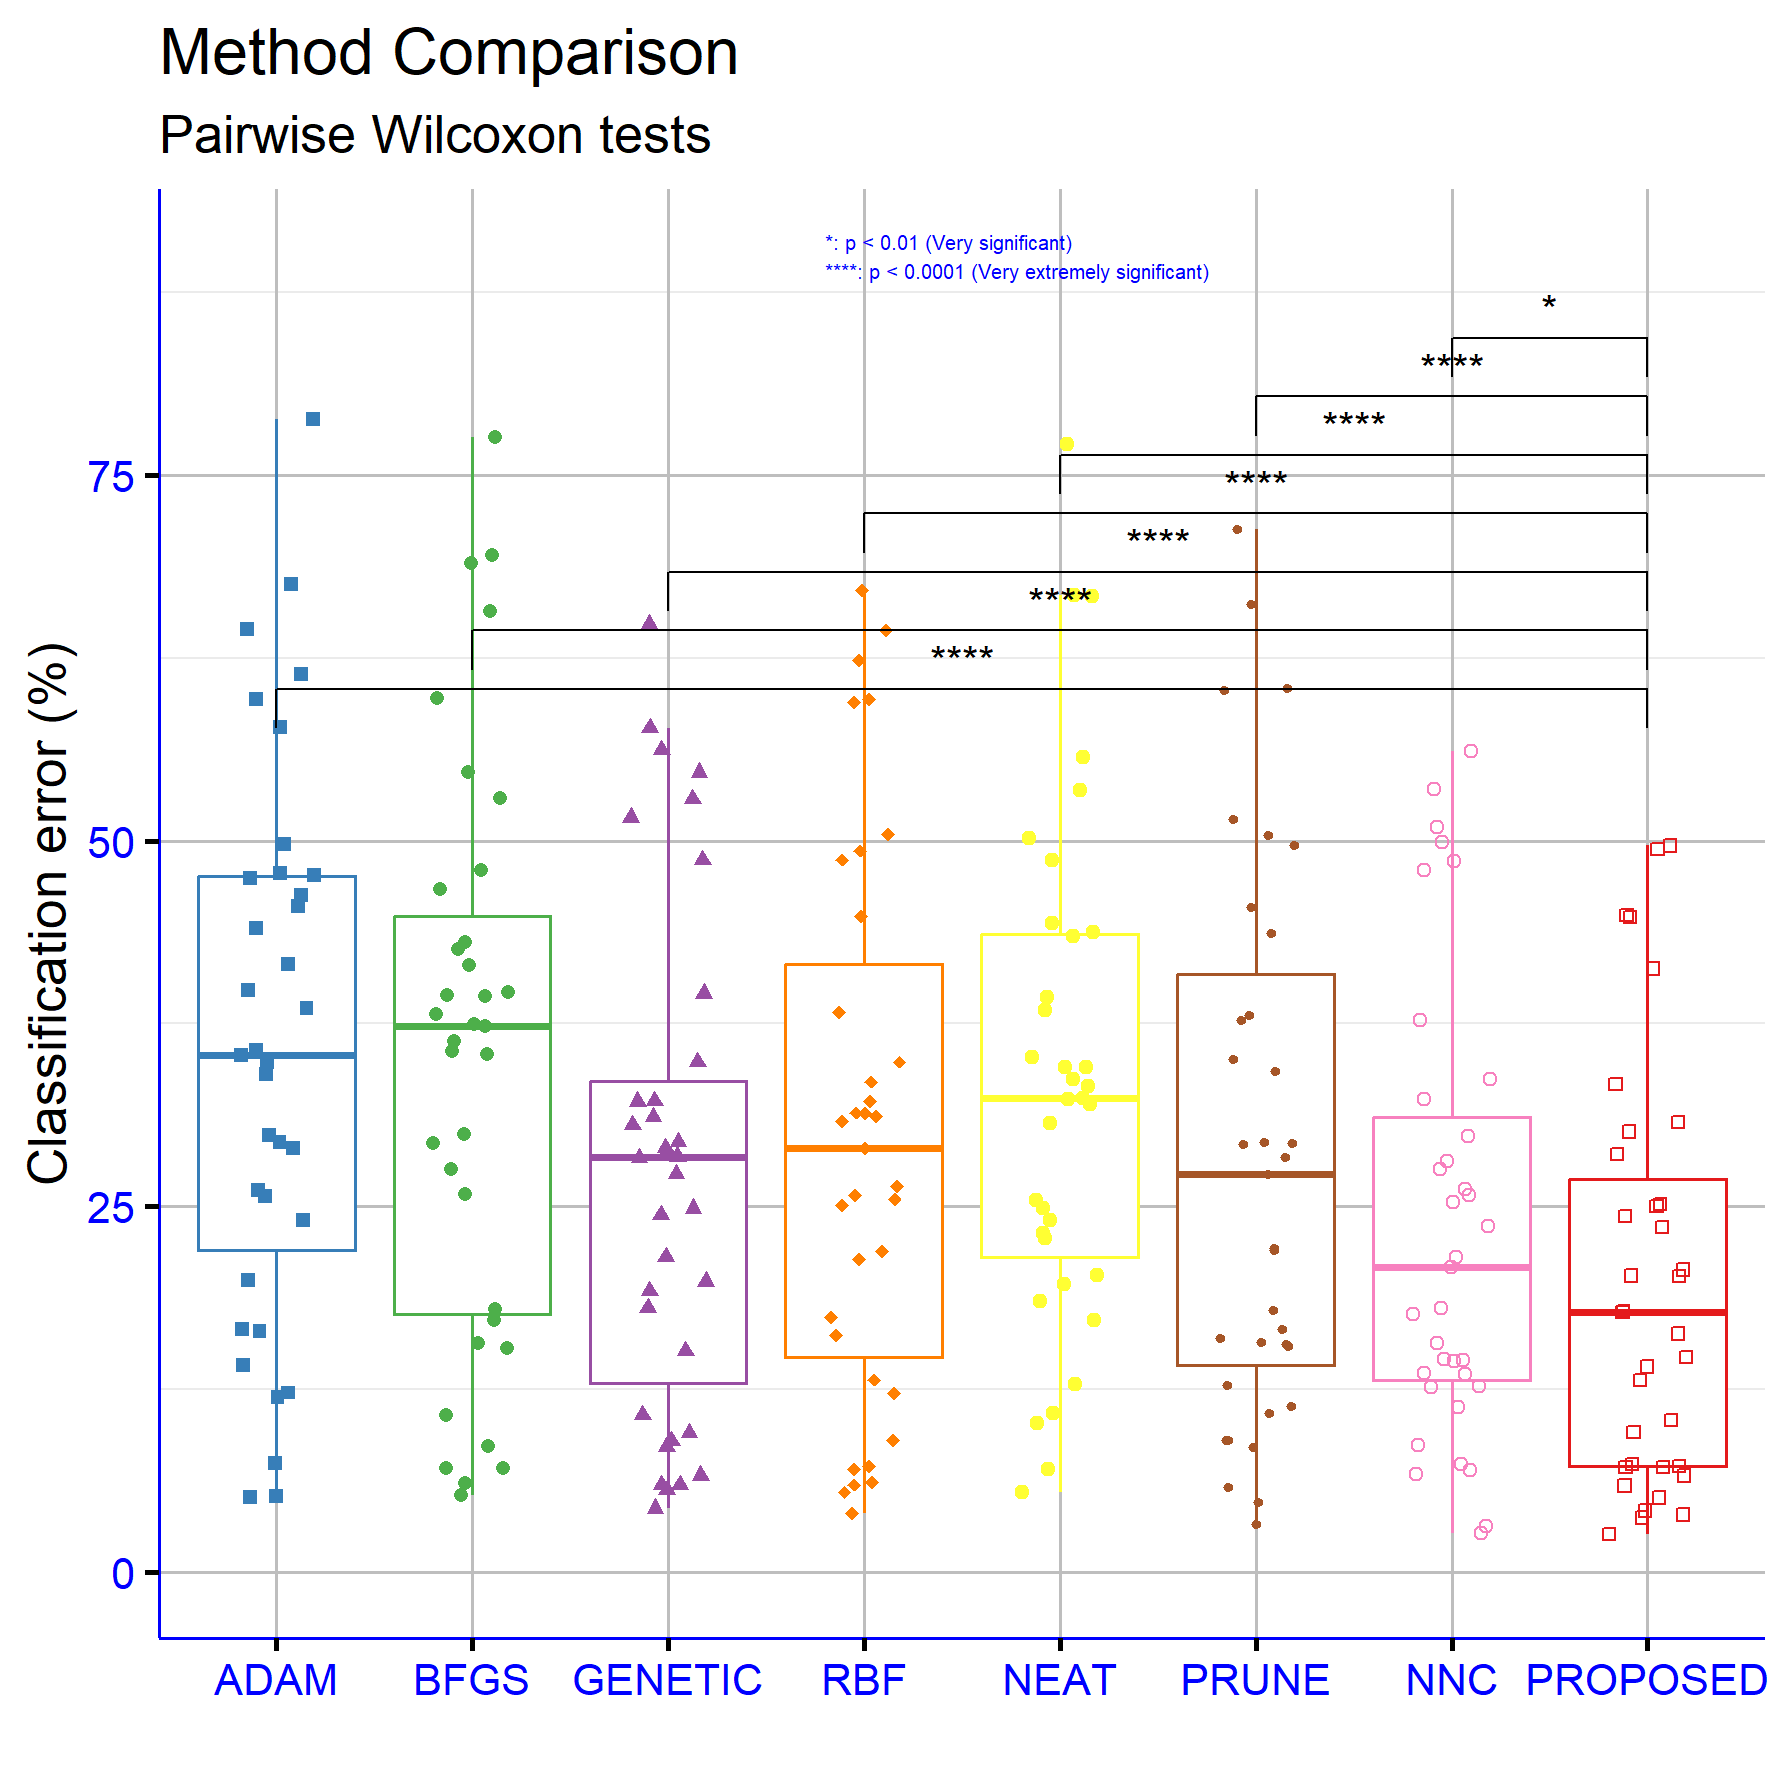
\includegraphics[scale=0.5]{stat1}
\par\end{centering}
\caption{Statistical analysis of the results obtained by various techniques
for the classification datasets.\label{fig:statClass}}

\end{figure}

From the analysis of the results presented in Figure \ref{fig:statRegression},
it is evident that the performance difference between the PROPOSED
model and BFGS is extremely significant (p \textless{} 0.0001), clearly
indicating the superiority of the PROPOSED model. Similarly, the comparisons
with GENETIC and NEAT show very high statistical significance (p \textless{}
0.001), confirming that the PROPOSED model achieves clearly better
results. The difference with NNC, though smaller, remains significant
(p \textless{} 0.01), showing that even in comparison with one of
the best-performing alternative models, the PROPOSED model still outperforms.
The differences with ADAM, RBF, and PRUNE are statistically significant
at the p \textless{} 0.05 level, suggesting a noteworthy advantage
of the PROPOSED model in these cases as well, albeit with a lower
confidence level. Overall, the statistical analysis of the regression
dataset results confirms the overall superiority of the PROPOSED model,
not only in terms of average prediction accuracy but also in the consistency
of its performance compared to the alternative approaches.

\begin{figure}[H]
\begin{centering}
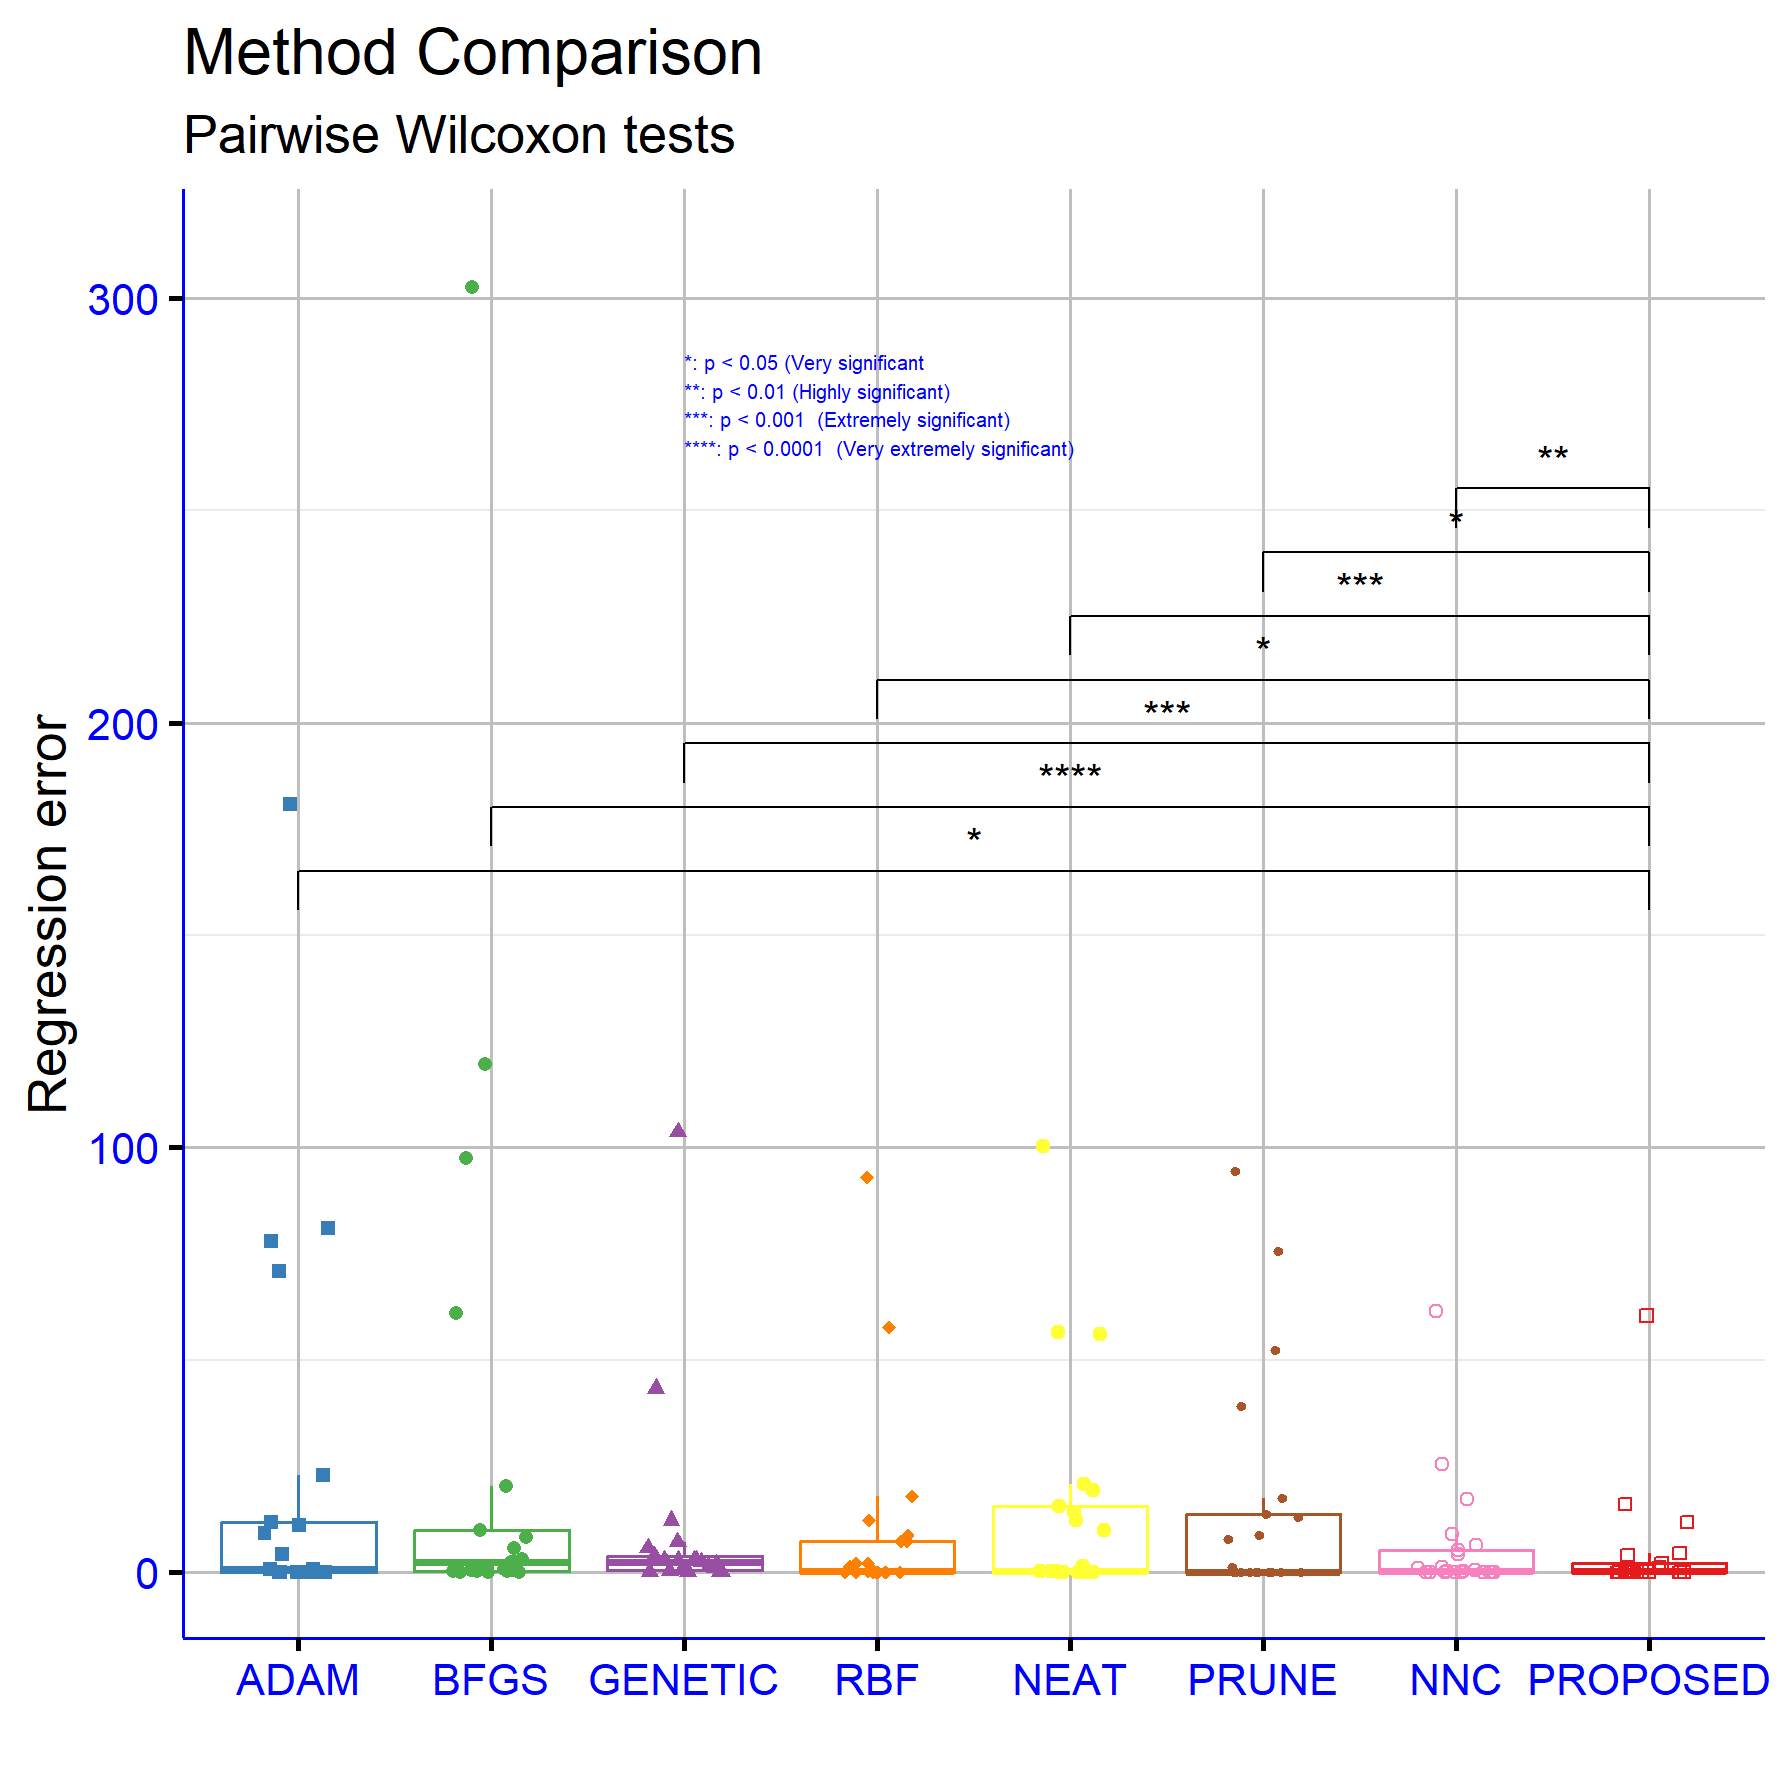
\includegraphics[scale=0.5]{stat2}
\par\end{centering}
\caption{Statistical analysis for the results obtained by the used techniques
on the regression datasets.\label{fig:statRegression}}

\end{figure}


\subsection{Experiments with the weight factor $I_{w}$}

An additional experiment was conducted, where the initial weight parameter
$I_{w}$, used in the first phase of the current work was altered
from 2 to 10. The purpose of this experiment is to determine the stability
of the proposed procedure to changes in this critical parameter.

Table \ref{tab:expClassIW} presents the error rates of the proposed
machine learning model on various classification datasets, considering
four different values of the parameter $I_{w}$ (initialization factor):
2, 3, 5, and 10. The recorded values correspond to error percentages
for each dataset, while the last row of the table includes the average
error rate for each parameter value. Analyzing the data, it is observed
that the value $I_{w}=10$ exhibits the lowest average error rate
(19.63\%), followed by $I_{w}=5$ (19.89\%). The values $I_{w}=2$
and $I_{w}=3$ have slightly higher averages, 20.32\% and 20.33\%
respectively. The difference between the averages is relatively small,
a fact suggesting that the parameter $I_{w}$ does not dramatically
affect the model's performance; however, the gradual decrease in average
error with increasing parameter value may indicate a trend of improvement.
\begin{table}[H]
\caption{Experimental results using the proposed method and different values
for the parameter $I_{w}$, which defines the number of parameters
for the initial phase of the method. The experiments were conducted
on the classification datasets.\label{tab:expClassIW}}

\centering{}{\footnotesize{}%
\begin{tabular}{|c|c|c|c|c|}
\hline 
DATASET & $I_{w}=2$ & $I_{w}=3$ & $I_{w}=5$ & $I_{w}=10$\tabularnewline
\hline 
\hline 
APPENDICITIS & 15.03\% & 15.67\% & 17.93\% & 16.30\%\tabularnewline
\hline 
ALCOHOL & 21.11\% & 25.63\% & 22.20\% & 20.21\%\tabularnewline
\hline 
AUSTRALIAN & 13.93\% & 14.01\% & 14.06\% & 14.68\%\tabularnewline
\hline 
BALANCE & 8.71\% & 8.91\% & 8.61\% & 7.26\%\tabularnewline
\hline 
CLEVELAND & 42.09\% & 42.24\% & 43.60\% & 44.90\%\tabularnewline
\hline 
CIRCULAR & 14.71\% & 6.93\% & 4.11\% & 4.22\%\tabularnewline
\hline 
DERMATOLOGY & 9.09\% & 6.78\% & 6.78\% & 5.92\%\tabularnewline
\hline 
ECOLI & 48.21\% & 56.21\% & 50.12\% & 44.79\%\tabularnewline
\hline 
GLASS & 54.76\% & 54.51\% & 52.40\% & 49.43\%\tabularnewline
\hline 
HABERMAN & 30.31\% & 29.11\% & 28.82\% & 28.57\%\tabularnewline
\hline 
HAYES-ROTH & 27.74\% & 31.31\% & 28.90\% & 30.77\%\tabularnewline
\hline 
HEART & 15.00\% & 15.32\% & 15.69\% & 17.85\%\tabularnewline
\hline 
HEARTATTACK & 18.61\% & 18.72\% & 19.17\% & 20.67\%\tabularnewline
\hline 
HOUSEVOTES & 5.80\% & 6.83\% & 6.88\% & 7.39\%\tabularnewline
\hline 
IONOSPHERE & 11.58\% & 15.16\% & 15.88\% & 13.14\%\tabularnewline
\hline 
LIVERDISORDER & 31.12\% & 31.70\% & 31.89\% & 33.38\%\tabularnewline
\hline 
LYMOGRAPHY & 21.76\% & 23.83\% & 26.84\% & 25.14\%\tabularnewline
\hline 
MAMMOGRAPHIC & 16.33\% & 16.49\% & 16.72\% & 17.77\%\tabularnewline
\hline 
PARKINSONS & 13.33\% & 13.47\% & 13.97\% & 14.05\%\tabularnewline
\hline 
PIMA & 23.57\% & 23.82\% & 23.76\% & 24.34\%\tabularnewline
\hline 
POPFAILURES & 4.98\% & 5.51\% & 7.11\% & 7.19\%\tabularnewline
\hline 
REGIONS2 & 24.63\% & 25.10\% & 25.58\% & 25.00\%\tabularnewline
\hline 
SAHEART & 29.41\% & 29.27\% & 30.48\% & 30.11\%\tabularnewline
\hline 
SEGMENT & 39.10\% & 24.74\% & 15.17\% & 9.59\%\tabularnewline
\hline 
SPIRAL & 47.10\% & 43.25\% & 42.66\% & 41.25\%\tabularnewline
\hline 
STATHEART & 18.06\% & 19.12\% & 19.01\% & 20.26\%\tabularnewline
\hline 
STUDENT & 3.73\% & 4.00\% & 4.54\% & 7.18\%\tabularnewline
\hline 
TRANSFUSION & 24.81\% & 24.38\% & 24.28\% & 23.59\%\tabularnewline
\hline 
WDBC & 3.25\% & 3.40\% & 3.60\% & 3.73\%\tabularnewline
\hline 
WINE & 9.08\% & 8.94\% & 9.37\% & 10.41\%\tabularnewline
\hline 
Z\_F\_S & 5.43\% & 5.53\% & 5.89\% & 6.60\%\tabularnewline
\hline 
Z\_O\_N\_F\_S & 48.60\% & 49.67\% & 48.79\% & 49.66\%\tabularnewline
\hline 
ZO\_NF\_S & 3.30\% & 3.11\% & 3.52\% & 3.94\%\tabularnewline
\hline 
ZONF\_S & 1.97\% & 2.06\% & 2.24\% & 2.60\%\tabularnewline
\hline 
ZOO & 5.13\% & 6.57\% & 5.63\% & 5.10\%\tabularnewline
\hline 
\textbf{AVERAGE} & \textbf{20.32\%} & \textbf{20.33\%} & \textbf{19.89\%} & \textbf{19.63\%}\tabularnewline
\hline 
\end{tabular}}{\footnotesize\par}
\end{table}

In individual datasets, small variations are observed depending on
the setting. In some cases, such as SEGMENT and CIRCULAR, increasing
the parameter value leads to noticeably better results. For example,
in SEGMENT the error rate decreases from 39.10\% for $I_{w}=2$ to
only 9.59\% for $I_{w}=10$. A similar improvement is observed in
CIRCULAR, where the error decreases from 14.71\% to 4.22\%. Conversely,
in other datasets the variation in values is smaller or negligible,
and in some cases, such as ECOLI and CLEVELAND, higher $I_{w}$ values
lead to slightly increased error. Overall, the statistical analysis
shows that although no statistically significant differences are observed
between the different parameter values, in accordance with the p-values
from previous analyses, there is nevertheless an indication that higher
values of $I_{w}$, such as 10, are associated with slightly improved
average performance and better results in certain datasets. This trend
may be interpreted as an indication that a higher initialization factor
might allow the model to start from more favourable learning conditions,
particularly in datasets with greater complexity. However, because
the variation is not systematic across all datasets, the selection
of the $I_{w}$ value should be done carefully and in relation to
the characteristics of each specific problem.

In Table \ref{tab:expRegressionIW}, a general trend of decreasing
average error is observed as the value of the initialization factor
$I_{w}$ increases. The average drops from 6.08 (for $I_{w}=2$) to
5.48 ($I_{w}=3$), 5.24 ($I_{w}=5$), and finally 4.83 ($I_{w}=10$).
This sequential decrease suggests that higher values of $I_{w}$ tend
to improve the model's overall performance. However, the effect is
not uniform across all datasets. In some cases, the improvement is
striking: in AUTO the error decreases from 17.16 ($I_{w}=2$) to 11.73
($I_{w}=10$), in HOUSING it reduces from 27.19 to 15.96, and in FRIEDMAN
the most noticeable improvement is recorded from 6.49 to 1.25. Additionally,
in STOCK a significant drop from 8.79 to 3.96 is observed. Conversely,
in some datasets performance deteriorates with increasing $I_{w}$:
in BASEBALL the error increases from 59.05 ($I_{w}=2$) to 60.42 ($I_{w}=10$)
and in LW from 0.11 to 0.32. In other datasets, such as AIRFOIL, LASER,
and PL, differences are minimal and practically negligible, with values
remaining very close for all $I_{w}$ parameters. For example, in
AIRFOIL all values are around 0.002, while in PL the difference between
values is merely 0.001. This heterogeneity in the response of different
datasets underscores that the optimal value of $I_{w}$ depends significantly
on the specific characteristics of each problem. Despite the general
improving trend with higher $I_{w}$ values, notable exceptions like
BASEBALL and LW confirm that there is no global optimal setting suitable
for all regression problems.

\begin{table}[H]
\caption{Experimental results using the proposed method and different values
for the parameter $I_{w}$, which is used for the number of parameters
for the initial phase of the method. The experiments were performed
on the regression datasets.\label{tab:expRegressionIW}}

\centering{}{\footnotesize{}%
\begin{tabular}{|c|c|c|c|c|}
\hline 
DATASET & $I_{w}=2$ & $I_{w}=3$ & $I_{w}=5$ & $I_{w}=10$\tabularnewline
\hline 
\hline 
ABALONE & 4.49 & 4.40 & 4.33 & 4.41\tabularnewline
\hline 
AIRFOIL & 0.002 & 0.002 & 0.002 & 0.001\tabularnewline
\hline 
AUTO & 17.16 & 16.14 & 14.55 & 11.73\tabularnewline
\hline 
BK & 0.13 & 0.18 & 0.12 & 0.058\tabularnewline
\hline 
BL & 0.005 & 0.19 & 0.14 & 0.13\tabularnewline
\hline 
BASEBALL & 59.05 & 52.43 & 54.83 & 60.42\tabularnewline
\hline 
CONCRETE & 0.005 & 0.004 & 0.003 & 0.004\tabularnewline
\hline 
DEE & 0.27 & 0.26 & 0.26 & 0.26\tabularnewline
\hline 
FRIEDMAN & 6.49 & 4.56 & 1.96 & 1.25\tabularnewline
\hline 
FY & 0.07 & 0.12 & 0.26 & 0.13\tabularnewline
\hline 
HO & 0.03 & 0.02 & 0.08 & 0.073\tabularnewline
\hline 
HOUSING & 27.19 & 25.53 & 21.47 & 15.96\tabularnewline
\hline 
LASER & 0.003 & 0.003 & 0.003 & 0.004\tabularnewline
\hline 
LW & 0.11 & 0.09 & 0.14 & 0.32\tabularnewline
\hline 
MORTGAGE & 0.25 & 0.25 & 0.19 & 0.15\tabularnewline
\hline 
PL & 0.022 & 0.021 & 0.021 & 0.021\tabularnewline
\hline 
PLASTIC & 3.17 & 2.33 & 2.18 & 2.15\tabularnewline
\hline 
QUAKE & 0.043 & 0.045 & 0.049 & 0.061\tabularnewline
\hline 
SN & 0.03 & 0.04 & 0.06 & 0.10\tabularnewline
\hline 
STOCK & 8.79 & 8.15 & 8.91 & 3.96\tabularnewline
\hline 
TREASURY & 0.39 & 0.40 & 0.38 & 0.25\tabularnewline
\hline 
\textbf{AVERAGE} & \textbf{6.08} & \textbf{5.48} & \textbf{5.24} & \textbf{4.83}\tabularnewline
\hline 
\end{tabular}}{\footnotesize\par}
\end{table}

Figure \ref{fig:statClassIW} presents the significance levels for
the comparison of different values of the $I_{w}$ (Initial weights)
parameter in classification datasets. The comparisons include the
pairs $I_{w}=2$ vs $I_{w}=3$, $I_{w}=3$ vs $I_{w}=5$, and $I_{w}=5$
vs $I_{w}=10$. In all cases, the p-values are greater than 0.05,
indicating that the differences between the respective settings are
not statistically significant. This implies that varying the $I_{w}$
parameter across these specific values does not substantially affect
the model's performance in classification tasks, and thus, no significant
changes in outcomes are observed due to this parameter.

\begin{figure}[H]
\begin{centering}
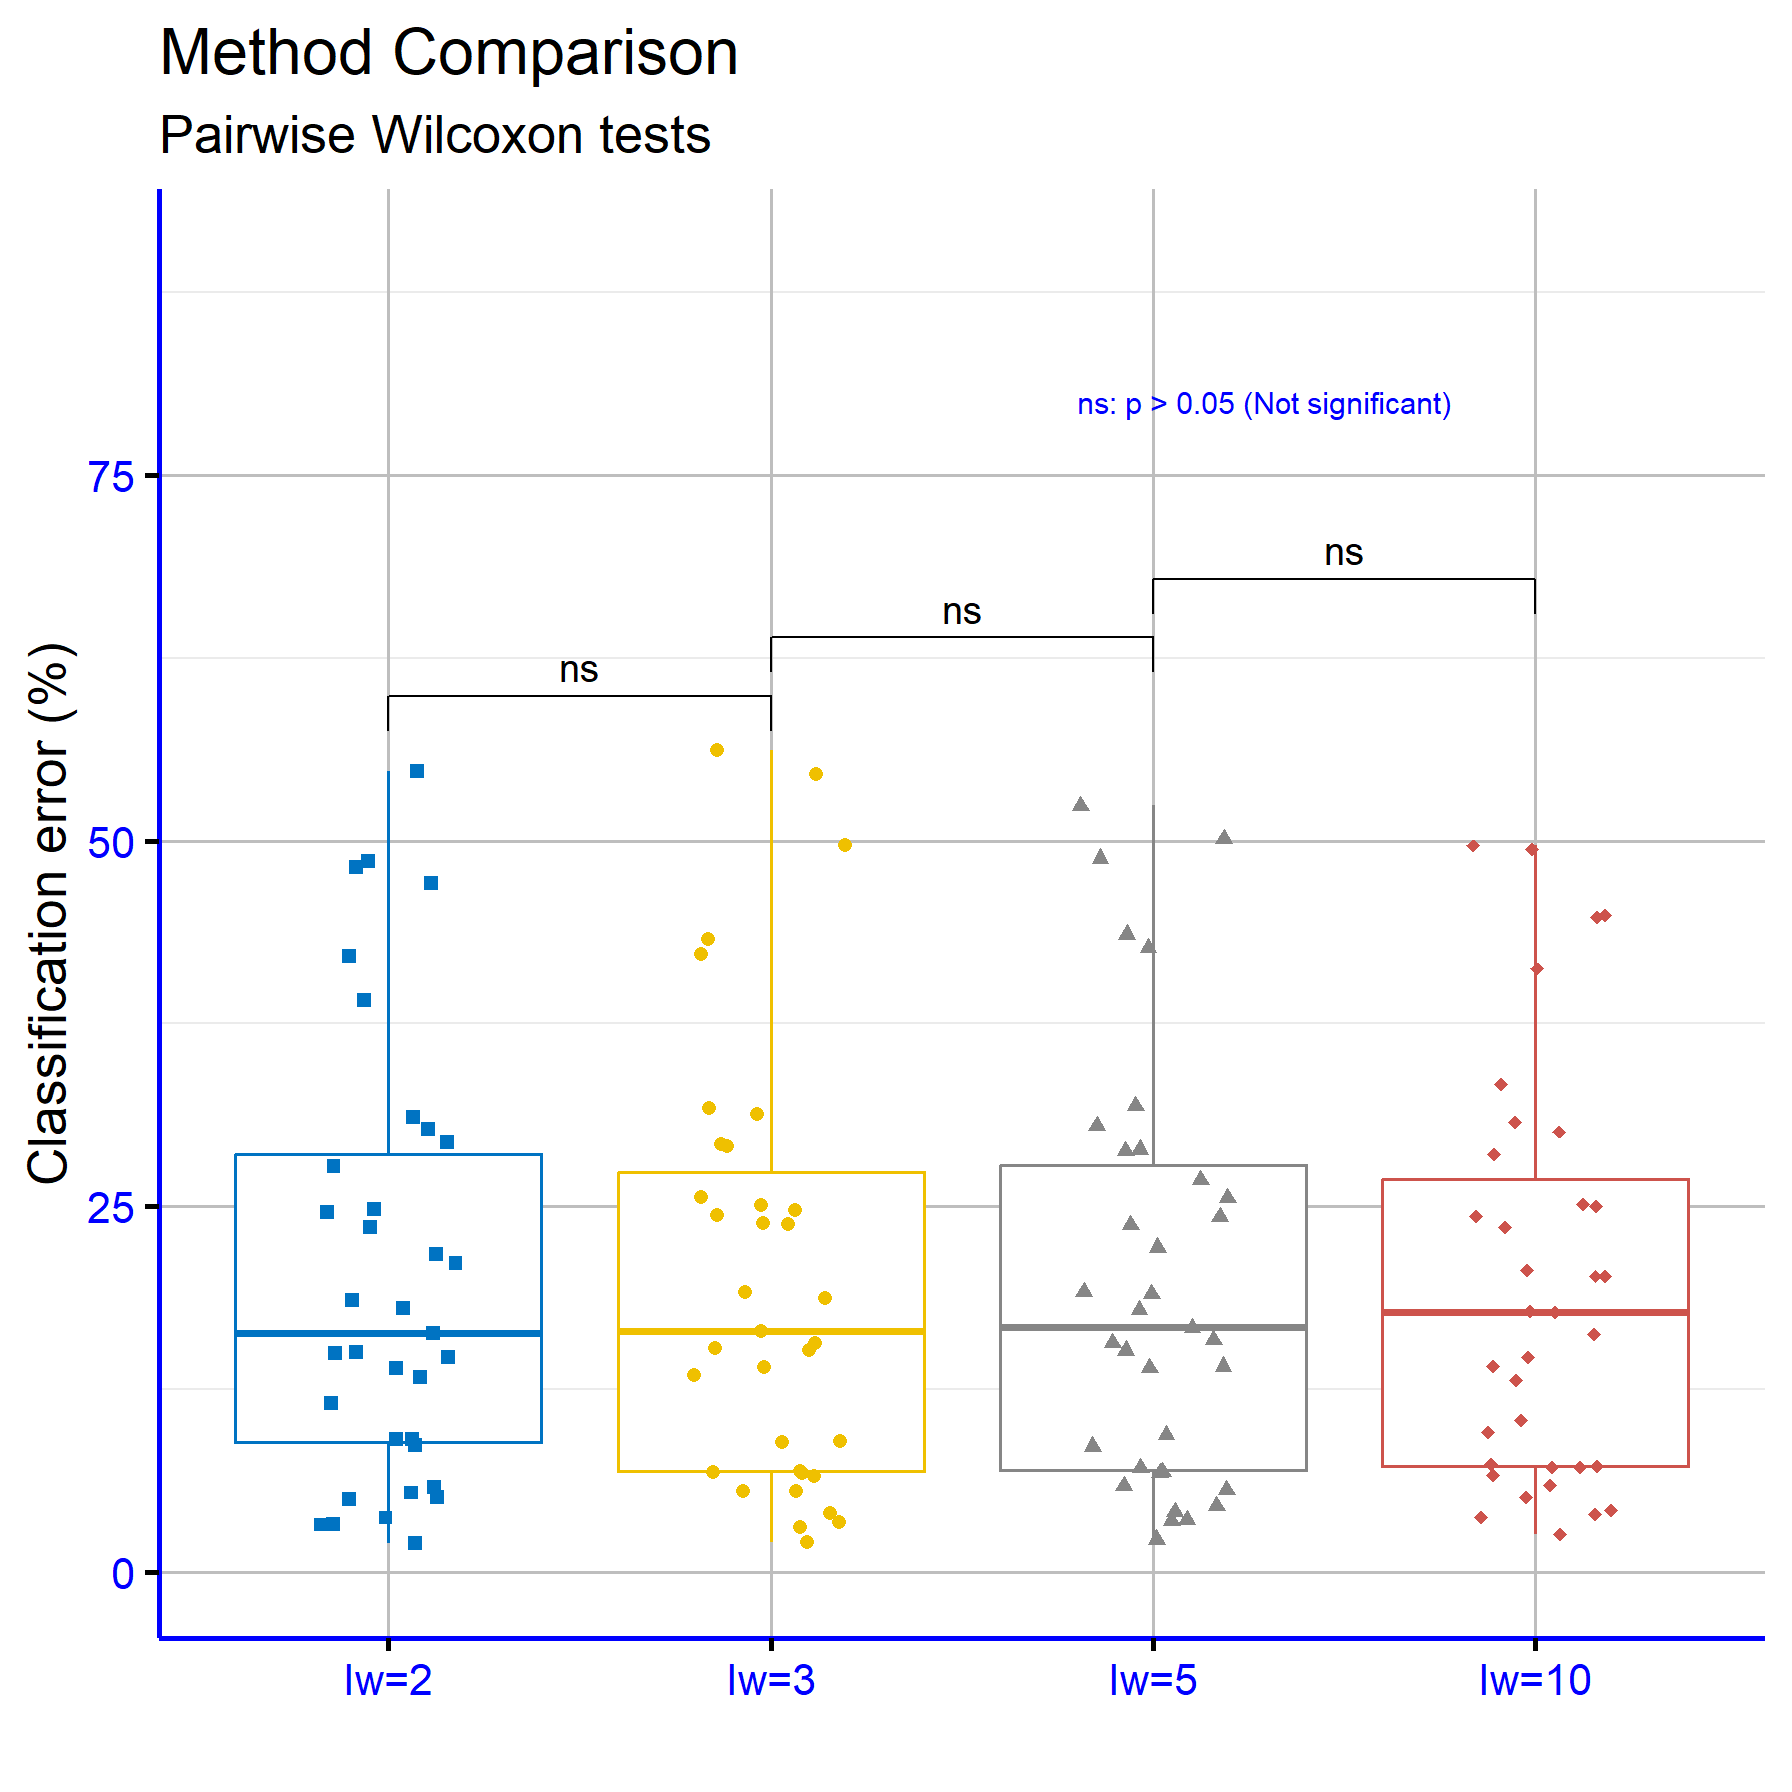
\includegraphics[scale=0.5]{stat3}
\par\end{centering}
\caption{Statistical comparison for the results obtained by the proposed method
and the series of values for $I_{w}$ parameter on the classification
datasets.\label{fig:statClassIW}}

\end{figure}

In Figure \ref{fig:statRegressionIW}, the statistical evaluation
focuses on how different initial weight settings ($I_{w}$) affect
performance in regression tasks. The comparisons between the values
$I_{w}=2$, $I_{w}=3$, $I_{w}=5$, and $I_{w}=10$ revealed no significant
variations, as all corresponding p-values were found to be greater
than 0.05. This outcome suggests that altering the $I_{w}$ parameter
within this range does not lead to measurable differences in the models’
predictive behavior. The results imply that model accuracy remains
stable regardless of these specific $I_{w}$ configurations in regression
scenarios.

\begin{figure}[H]
\begin{centering}
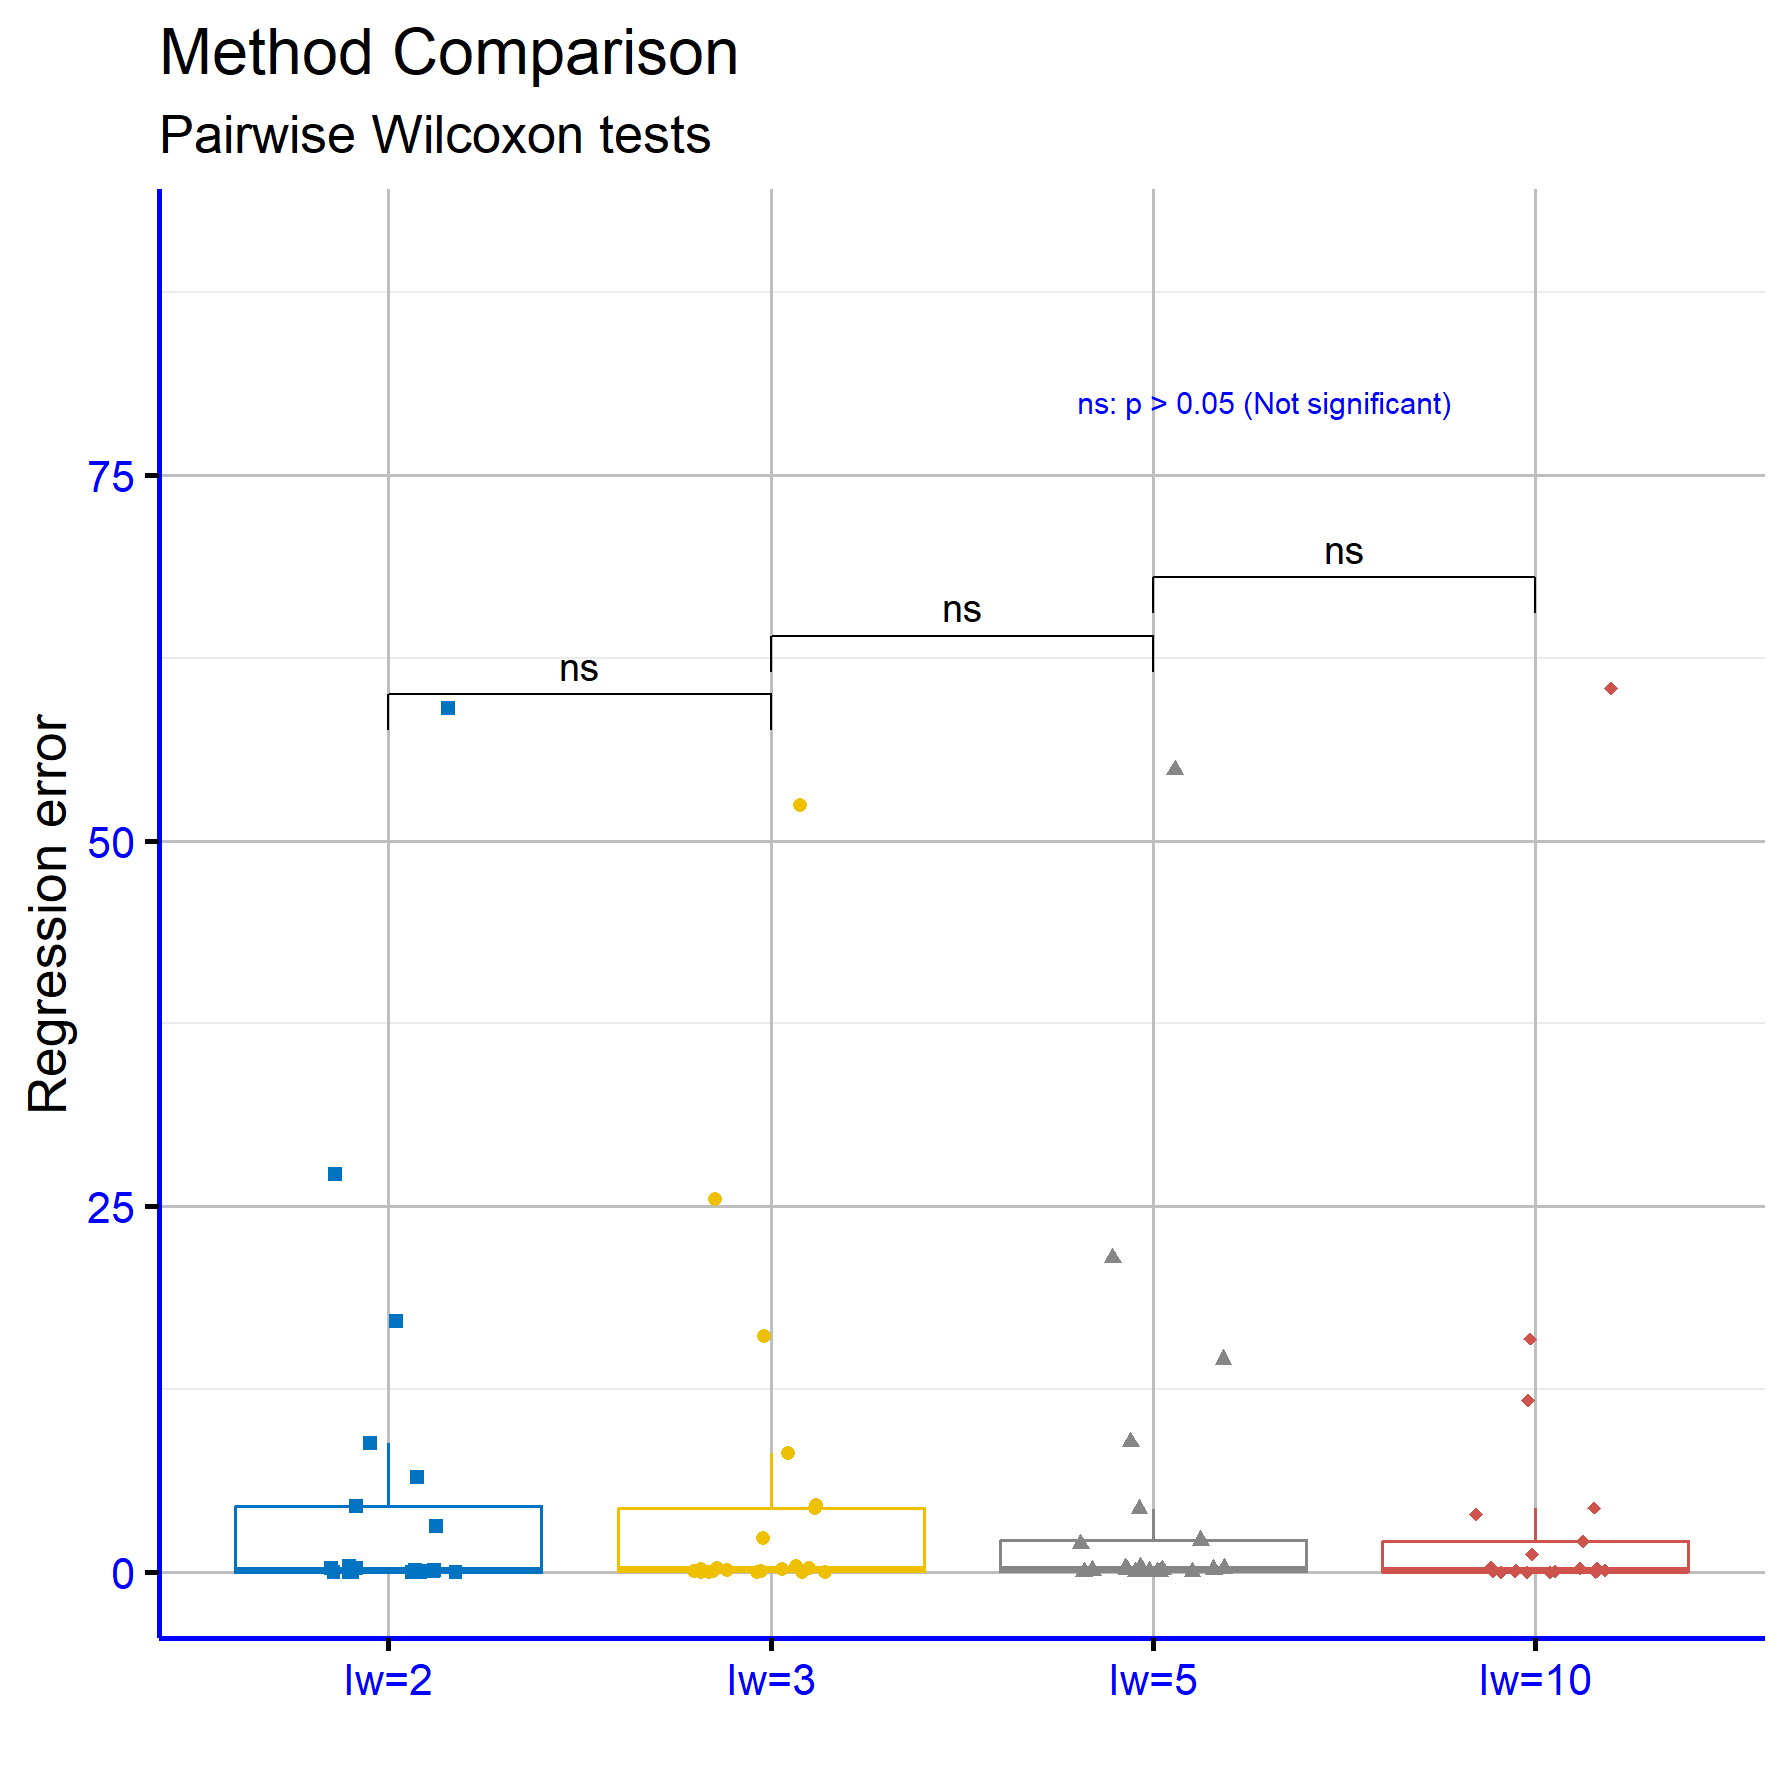
\includegraphics[scale=0.5]{stat4}
\par\end{centering}
\caption{Statistical comparison for the results obtained by the proposed method
on the regression datasets, using a variety of values for the parameter
$I_{w}$.\label{fig:statRegressionIW}}

\end{figure}
A comparison in terms of precision and recall between the original
neural network construction method and the proposed one is outlined
in Figure \ref{fig:precisionAndRecall}.

\begin{figure}[H]
\begin{centering}
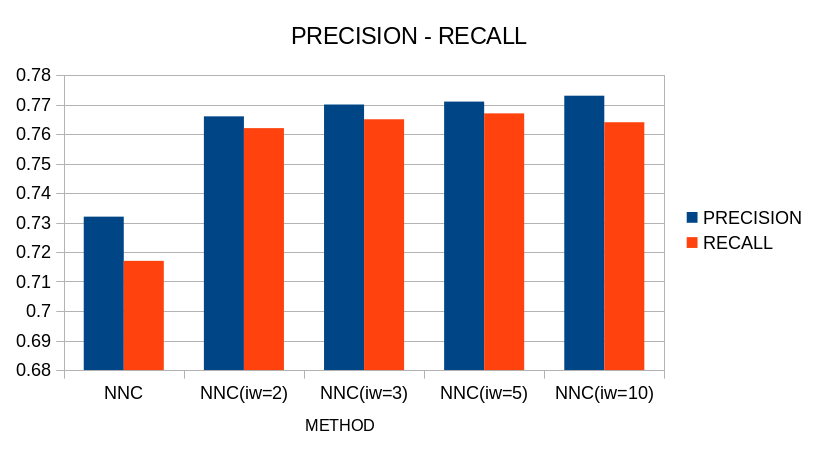
\includegraphics[scale=0.75]{pre_precision_recall}
\par\end{centering}
\caption{Comparison in terms of precision and recall between the original neural
network construction method and the proposed one. In the experiments
the following values for the critical parameter $I_{w}$ were used:
2,3,5 and 10.\label{fig:precisionAndRecall}}

\end{figure}
As can be clearly seen from this figure, the proposed technique significantly
improves the performance of the artificial neural network construction
method on classification data, achieving high rates of correct data
classification.

Although the proposed technique appears to be more efficient than
the original one, the addition of the first processing phase results
in a significant increase in execution time, as also demonstrated
in Figure \ref{fig:Average-execution-time}.

\begin{figure}[H]
\begin{centering}
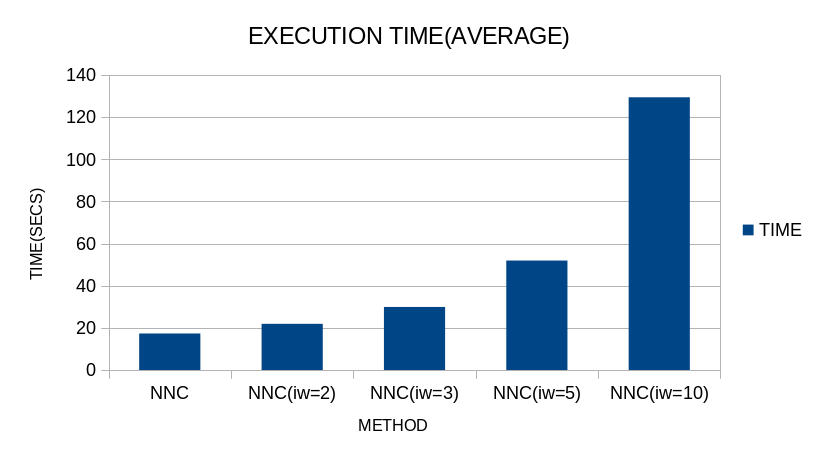
\includegraphics[scale=0.75]{pre_time}
\par\end{centering}
\caption{Average execution time for the classification datasets using the original
neural network construction method and the proposed one with different
values of the critical factor $I_{w}$.\label{fig:Average-execution-time}}

\end{figure}
It is clear that there is a significant increase in execution time,
as more units are added to the initial neural network of the first
phase, and in fact this time increases significantly between the values
$I_{w}=5$ and $I_{w}=10$.

\subsection{Some real world examples}

As real world examples with many instances consider the the PIRvision
dataset, initially discussed in 2023 \citep{pirvision} and the Beed
dataset presented in the work of Banu \citep{beed}. 

This PIRvision dataset contains occupancy detection data that was
collected from a Synchronized Low-Energy Electronically-chopped Passive
Infra-Red sensing node in residential and office environments. The
dataset contains 15302 patterns and the dimension of each pattern
is 59. The Beed dataset (Bangalore EEG Epilepsy Dataset) is a comprehensive
EEG collection for epileptic seizure detection and classification
and contains 8000 patterns and each pattern has 16 features. In the
conducted experiments the following methods were used:
\begin{enumerate}
\item BFGS, that defines the BFGS method incorporated to train a neural
network with $H=10$ processing nodes.
\item GENETIC, which is used to represent a genetic algorithm used to train
a neural network with $H=10$ processing nodes.
\item NNC, that represents the initial neural network construction method.
\item The proposed method with the following values for $I_{w}$ parameter:
$I_{w}=2,\ I_{w}=3,\ I_{w}=5$ and $I_{w}=10$.
\end{enumerate}
The results were validated using the ten - fold cross validation method.
For the PIRVision datasets the results are depicted in Figure \ref{fig:pirvision}.

\begin{figure}[H]
\begin{centering}
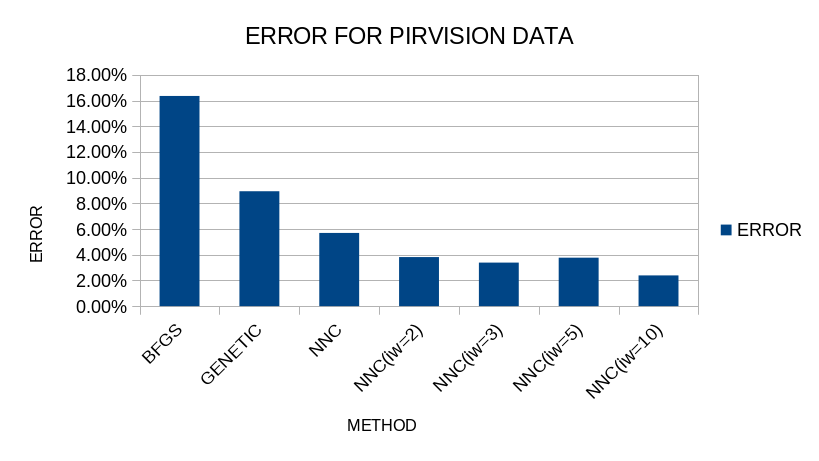
\includegraphics[scale=0.75]{pirvision}
\par\end{centering}
\caption{Results obtained for the PIRvision dataset, using a variety of methods
and the proposed one. The numbers in the graph indicate average classification
error as measured on the test set.\label{fig:pirvision}}

\end{figure}
As is evident from the specific results, the artificial neural network
construction technique significantly outperforms the others and in
fact the proposed procedure significantly improves the results, especially
in the case where the parameter $I_{w}$ takes the value 10, where
the average classification error reaches approximately 2\%.

The results for the BEED dataset are outlined in Figure \ref{fig:beed}.

\begin{figure}[H]
\begin{centering}
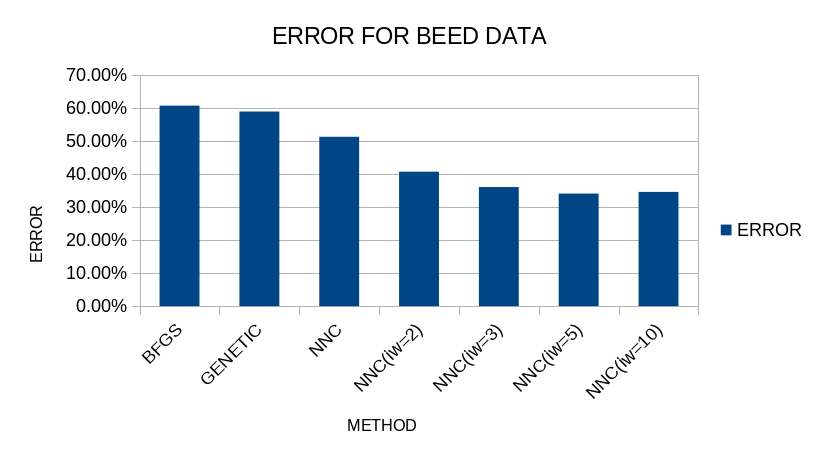
\includegraphics[scale=0.75]{beed}
\par\end{centering}
\caption{Results obtained for the BEED dataset. The numbers in the graph indicate
average classification error as measured on the test set.\label{fig:beed}}

\end{figure}
And in this case, the proposed method significantly reduces the data
classification error compared to a simple genetic algorithm or compared
to the original method of constructing artificial neural networks.

\subsection{Experiments with the number of chromosomes $N_{c}$}

Additionally, another experiment was conducted using the proposed
method and a range of values for the critical parameter $N_{c}$,
which represents the number of used chromosomes. Table \ref{tab:expClassNC}
presents the classification error rates of the proposed machine learning
method across various datasets, for four different values of $N_{c}$,
which corresponds to the number of chromosomes used in the evolutionary
process. It is observed that, in a large proportion of datasets, an
increase in $N_{c}$ is accompanied by a reduction in the error rate,
indicating that a greater diversity of initial solutions can lead
to better final performance. In certain datasets, such as DERMATOLOGY,
ECOLI, SEGMENT, and Z\_F\_S, the improvement is particularly evident
at higher $N_{c}$ values, whereas in others, such as AUSTRALIAN,
HEART, and MAMMOGRAPHIC, the change is small or nonexistent, suggesting
that performance in these cases is less sensitive to an increase in
the number of chromosomes. There are also instances where increasing
$N_{c}$ does not lead to improvement but rather to a slight increase
in error, as in GLASS and CIRCULAR, a phenomenon that may be due to
overfitting or random variation in performance. The mean percentage
error gradually decreases from 21.40\% for $N_{c}=50$ to 19.63\%
for $N_{c}=500$, confirming the general trend of improvement with
increasing $N_{c}$, although the benefit from very large values appears
to diminish, possibly indicating saturation in the model’s ability
to exploit the additional diversity. Overall, the statistical picture
shows that increasing the number of chromosomes contributes to reducing
the error, but the degree of benefit depends on the characteristics
of each dataset.

\begin{table}[H]
\caption{Experimental results using the proposed method and different values
for the parameter $N_{c}$, which indicates the number of chromosomes
used in the genetic algorithm. . The experiments were conducted on
the classification datasets.\label{tab:expClassNC}}

\centering{}{\footnotesize{}%
\begin{tabular}{|c|c|c|c|c|}
\hline 
DATASET & $N_{c}=50$ & $N_{c}=100$ & $N_{c}=200$ & $N_{c}=500$\tabularnewline
\hline 
\hline 
APPENDICITIS & 20.80\% & 20.50\% & 18.50\% & 16.30\%\tabularnewline
\hline 
ALCOHOL & 24.74\% & 28.47\% & 20.85\% & 20.21\%\tabularnewline
\hline 
AUSTRALIAN & 14.26\% & 14.40\% & 14.68\% & 14.68\%\tabularnewline
\hline 
BALANCE & 7.71\% & 7.79\% & 6.82\% & 7.26\%\tabularnewline
\hline 
CLEVELAND & 45.03\% & 43.86\% & 44.42\% & 44.90\%\tabularnewline
\hline 
CIRCULAR & 4.67\% & 4.02\% & 4.08\% & 4.22\%\tabularnewline
\hline 
DERMATOLOGY & 10.26\% & 7.71\% & 6.11\% & 5.92\%\tabularnewline
\hline 
ECOLI & 54.70\% & 49.30\% & 44.18\% & 44.79\%\tabularnewline
\hline 
GLASS & 50.48\% & 52.33\% & 49.62\% & 49.43\%\tabularnewline
\hline 
HABERMAN & 29.57\% & 29.40\% & 29.10\% & 28.57\%\tabularnewline
\hline 
HAYES-ROTH & 32.47\% & 31.16\% & 31.62\% & 30.77\%\tabularnewline
\hline 
HEART & 18.34\% & 17.63\% & 17.85\% & 17.85\%\tabularnewline
\hline 
HEARTATTACK & 20.07\% & 21.00\% & 20.67\% & 20.67\%\tabularnewline
\hline 
HOUSEVOTES & 7.09\% & 8.22\% & 7.44\% & 7.39\%\tabularnewline
\hline 
IONOSPHERE & 16.91\% & 16.69\% & 15.79\% & 13.14\%\tabularnewline
\hline 
LIVERDISORDER & 33.77\% & 32.06\% & 33.50\% & 33.38\%\tabularnewline
\hline 
LYMOGRAPHY & 25.36\% & 24.86\% & 25.72\% & 25.14\%\tabularnewline
\hline 
MAMMOGRAPHIC & 17.23\% & 17.67\% & 17.81\% & 17.77\%\tabularnewline
\hline 
PARKINSONS & 13.37\% & 15.53\% & 14.95\% & 14.05\%\tabularnewline
\hline 
PIMA & 25.82\% & 24.64\% & 24.50\% & 24.34\%\tabularnewline
\hline 
POPFAILURES & 7.74\% & 7.39\% & 7.17\% & 7.19\%\tabularnewline
\hline 
REGIONS2 & 28.53\% & 27.29\% & 25.78\% & 25.00\%\tabularnewline
\hline 
SAHEART & 31.70\% & 30.74\% & 30.15\% & 30.11\%\tabularnewline
\hline 
SEGMENT & 16.29\% & 12.16\% & 9.08\% & 9.59\%\tabularnewline
\hline 
SPIRAL & 41.93\% & 42.04\% & 41.19\% & 41.25\%\tabularnewline
\hline 
STATHEART & 20.30\% & 19.67\% & 21.15\% & 20.26\%\tabularnewline
\hline 
STUDENT & 6.73\% & 7.25\% & 7.13\% & 7.18\%\tabularnewline
\hline 
TRANSFUSION & 25.15\% & 23.86\% & 23.69\% & 23.59\%\tabularnewline
\hline 
WDBC & 4.14\% & 4.16\% & 3.73\% & 3.73\%\tabularnewline
\hline 
WINE & 10.06\% & 10.65\% & 11.00\% & 10.41\%\tabularnewline
\hline 
Z\_F\_S & 12.73\% & 6.70\% & 6.27\% & 6.60\%\tabularnewline
\hline 
Z\_O\_N\_F\_S & 53.26\% & 55.78\% & 51.14\% & 49.66\%\tabularnewline
\hline 
ZO\_NF\_S & 8.12\% & 3.98\% & 3.66\% & 3.94\%\tabularnewline
\hline 
ZONF\_S & 2.70\% & 2.64\% & 2.66\% & 2.60\%\tabularnewline
\hline 
ZOO & 6.90\% & 6.80\% & 4.80\% & 5.10\%\tabularnewline
\hline 
\textbf{AVERAGE} & \textbf{21.40\%} & \textbf{20.81\%} & \textbf{19.91\%} & \textbf{19.63\%}\tabularnewline
\hline 
\end{tabular}}{\footnotesize\par}
\end{table}
Table \ref{tab:expRegressionNC} presents the absolute prediction
errors of the proposed machine learning method across various regression
datasets, for four different values of $N_{c}$, which represents
the number of chromosomes in the evolutionary process. The general
trend observed is a reduction in error as $N_{c}$ increases, suggesting
that greater solution diversity leads to more accurate predictions.
This is particularly evident in datasets such as AUTO, BL, HOUSING,
STOCK, and TREASURY, where the difference between $N_{c}=50$ and
$N_{c}=500$ is substantial. In some datasets, such as ABALONE, AIRFOIL,
CONCRETE, and LASER, the values remain almost unchanged regardless
of $N_{c}$, indicating that performance in these cases is less dependent
on the number of chromosomes. There are also cases with non-monotonic
behavior, such as BK and LW, where increasing $N_{c}$ does not necessarily
lead to a consistent reduction in error, possibly due to stochastic
factors or overfitting. The mean error steadily decreases from 5.78
for $N_{c}=50$ to 4.83 for $N_{c}=500$, reinforcing the overall
picture of improvement, although the difference between the two largest
$N_{c}$ values is smaller, which may indicate that the benefit of
increasing $N_{c}$ begins to saturate. Overall, the statistical analysis
shows that increasing the number of chromosomes improves the accuracy
of the method, with the magnitude of the benefit depending on the
specific characteristics of each dataset.

\begin{table}[H]
\caption{Experimental results using the proposed method and different values
for the parameter $N_{c}$, used to represent the number of chromosomes
in the genetic population. The experiments were performed on the regression
datasets.\label{tab:expRegressionNC}}

\centering{}{\footnotesize{}%
\begin{tabular}{|c|c|c|c|c|}
\hline 
DATASET & $N_{c}=50$ & $N_{c}=100$ & $N_{c}=200$ & $N_{c}=500$\tabularnewline
\hline 
\hline 
ABALONE & 4.35 & 4.38 & 4.34 & 4.41\tabularnewline
\hline 
AIRFOIL & 0.001 & 0.001 & 0.001 & 0.001\tabularnewline
\hline 
AUTO & 18.99 & 16.57 & 11.25 & 11.73\tabularnewline
\hline 
BK & 0.044 & 0.344 & 0.14 & 0.058\tabularnewline
\hline 
BL & 0.81 & 0.77 & 0.45 & 0.13\tabularnewline
\hline 
BASEBALL & 62.38 & 63.29 & 68.56 & 60.42\tabularnewline
\hline 
CONCRETE & 0.004 & 0.004 & 0.004 & 0.004\tabularnewline
\hline 
DEE & 0.33 & 0.33 & 0.28 & 0.26\tabularnewline
\hline 
FRIEDMAN & 1.24 & 1.24 & 1.23 & 1.25\tabularnewline
\hline 
FY & 0.33 & 0.21 & 0.26 & 0.13\tabularnewline
\hline 
HO & 0.046 & 0.10 & 0.22 & 0.073\tabularnewline
\hline 
HOUSING & 21.71 & 22.05 & 15.97 & 15.96\tabularnewline
\hline 
LASER & 0.003 & 0.003 & 0.003 & 0.004\tabularnewline
\hline 
LW & 0.30 & 0.31 & 0.68 & 0.32\tabularnewline
\hline 
MORTGAGE & 0.36 & 0.20 & 0.16 & 0.15\tabularnewline
\hline 
PL & 0.027 & 0.021 & 0.021 & 0.021\tabularnewline
\hline 
PLASTIC & 2.92 & 2.18 & 2.11 & 2.15\tabularnewline
\hline 
QUAKE & 0.076 & 0.065 & 0.059 & 0.061\tabularnewline
\hline 
SN & 0.30 & 0.19 & 0.14 & 0.10\tabularnewline
\hline 
STOCK & 6.69 & 5.23 & 4.66 & 3.96\tabularnewline
\hline 
TREASURY & 0.56 & 0.53 & 0.30 & 0.25\tabularnewline
\hline 
\textbf{AVERAGE} & \textbf{5.78} & \textbf{5.62} & \textbf{5.28} & \textbf{4.83}\tabularnewline
\hline 
\end{tabular}}{\footnotesize\par}
\end{table}
Figure \ref{fig:statClassNC} presents the significance levels resulting
from the comparisons of classification error rates across datasets
for the proposed machine learning method. The comparison between $N_{c}=50$
and $N_{c}=100$ shows no significant difference (p=ns), indicating
that increasing the number of chromosomes from 50 to 100 does not
lead to a substantial improvement. In contrast, the transition from
$N_{c}=100$ to $N_{c}=200$ shows a statistically significant improvement
(p={*}{*}), while the increase from $N_{c}=200$ to $N_{c}=500$ is
also accompanied by a significant difference (p={*}), albeit of lower
magnitude. These results suggest that higher $N_{c}$ values can improve
performance, with the significance being more pronounced in the mid-range
$N_{c}$ values.

\begin{figure}[H]
\begin{centering}
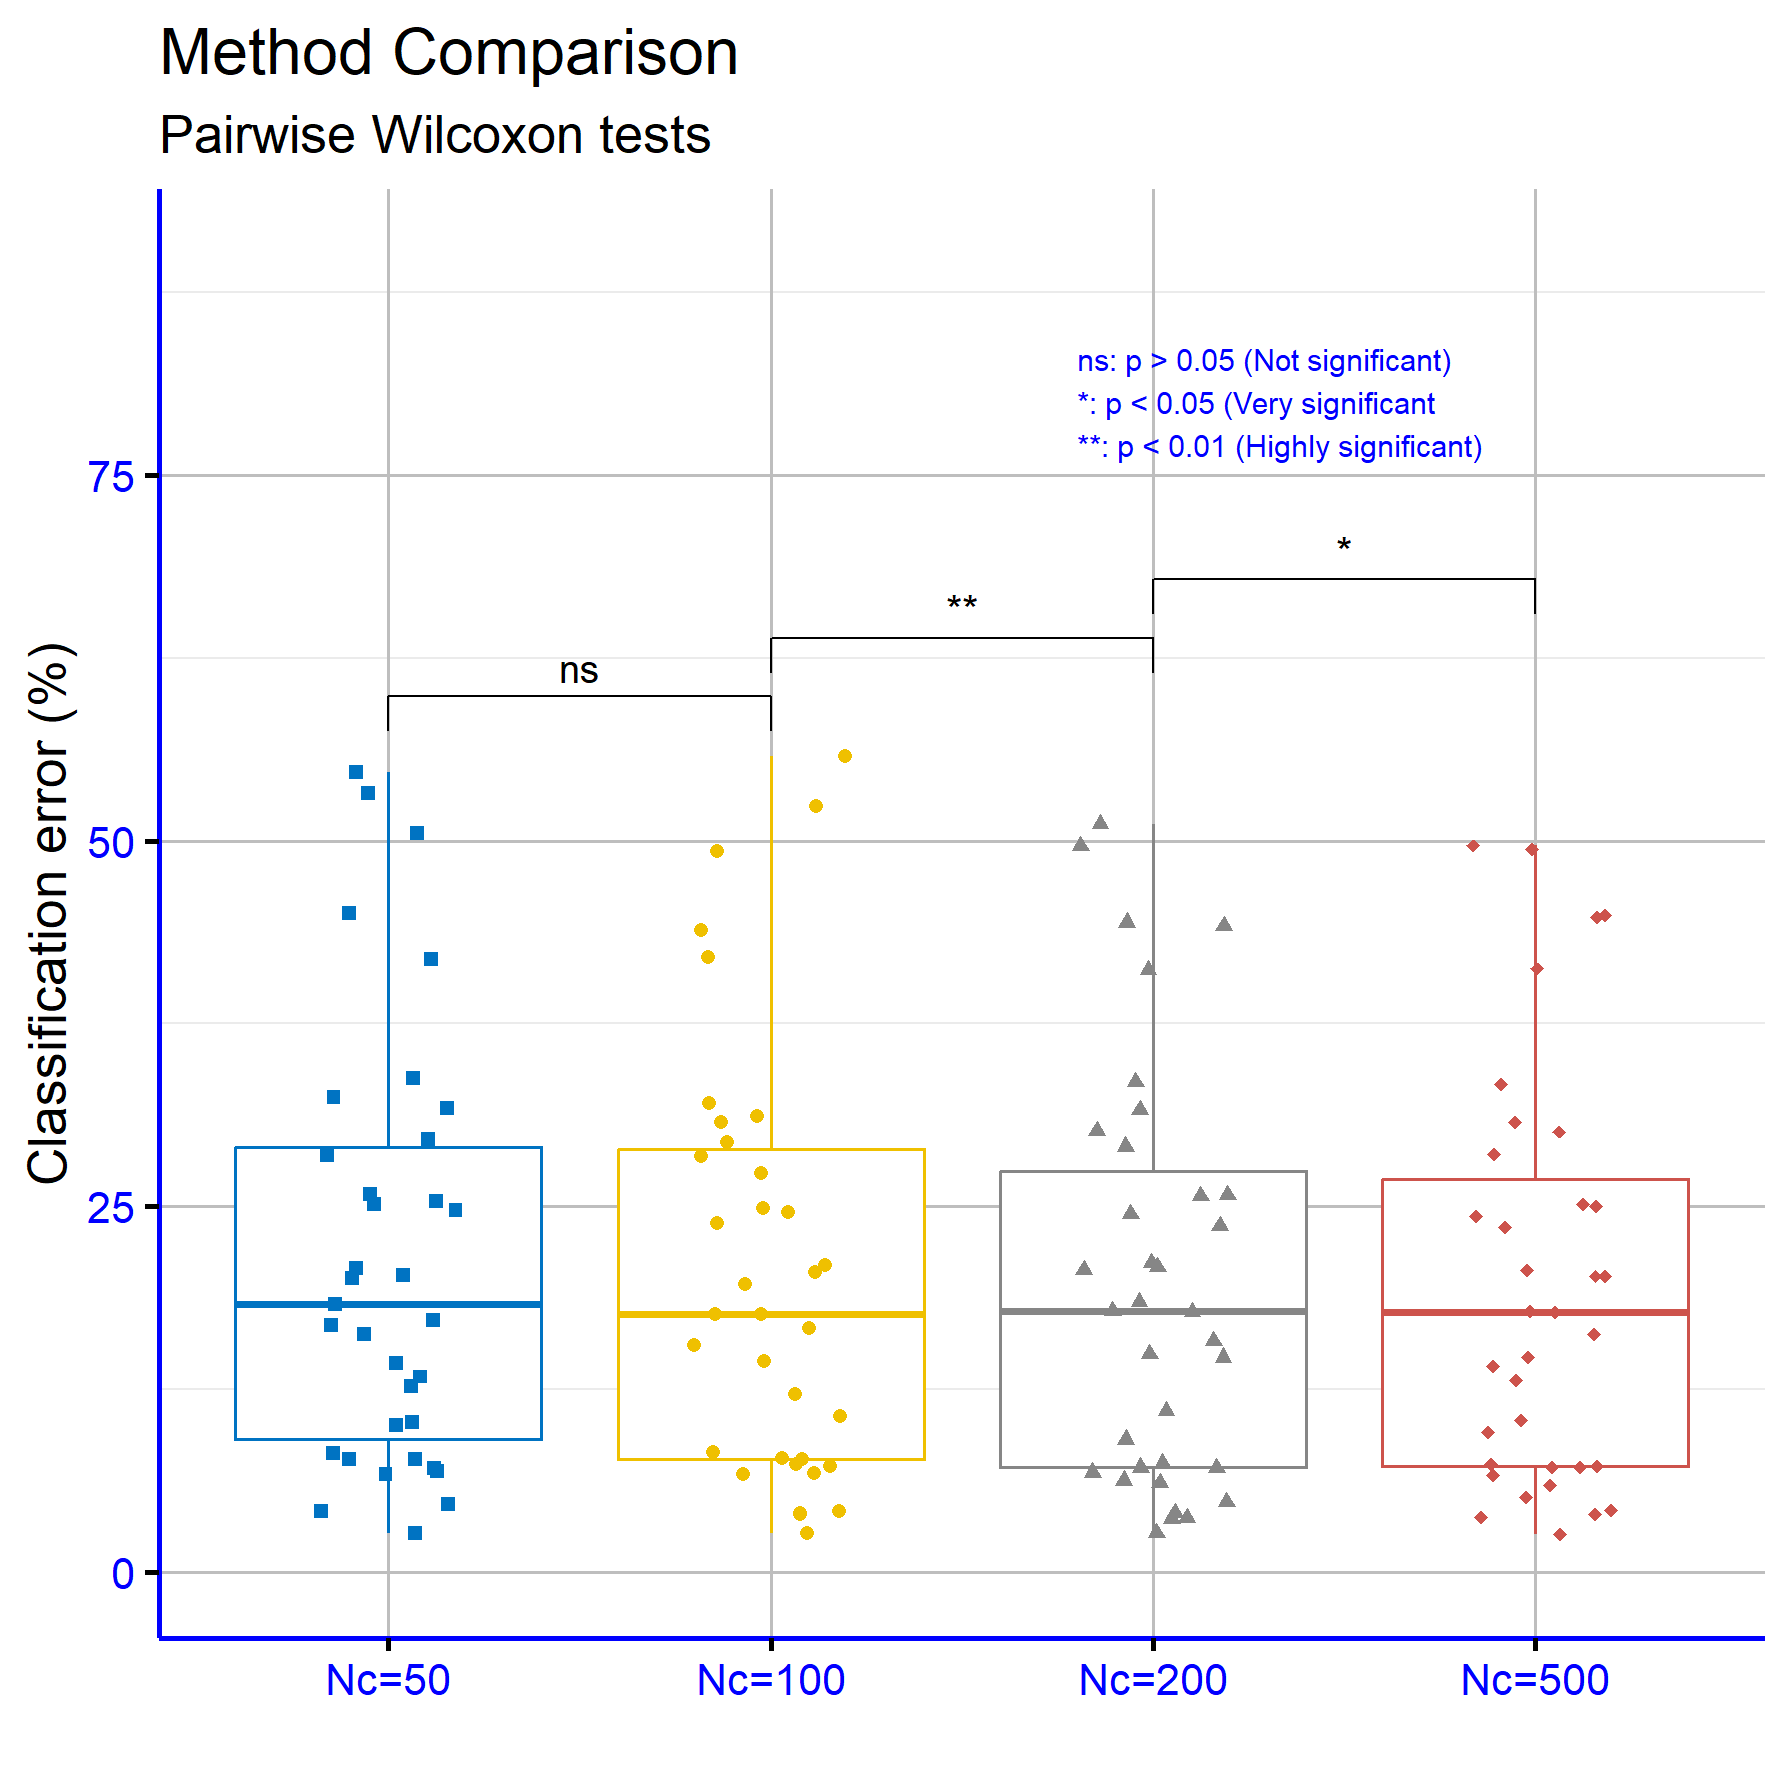
\includegraphics[scale=0.5]{stat6}
\par\end{centering}
\caption{Statistical comparison for the results obtained by the application
of the proposed method on the classification datasets using a range
of values for the parameter $N_{c}$.\label{fig:statClassNC}}

\end{figure}
Figure \ref{fig:statRegressionNC} presents the significance levels
resulting from the comparisons of prediction errors across regression
datasets for the proposed machine learning method. In all three comparisons
between $N_{c}=50$ and $N_{c}=100$, $N_{c}=100$ and $N_{c}=200$,
as well as $N_{c}=200$ and $N_{c}=500$ the p-value is non-significant
(p=ns), indicating that increasing the number of chromosomes does
not lead to a statistically significant change in the model’s performance
on these datasets.
\begin{figure}[H]
\begin{centering}
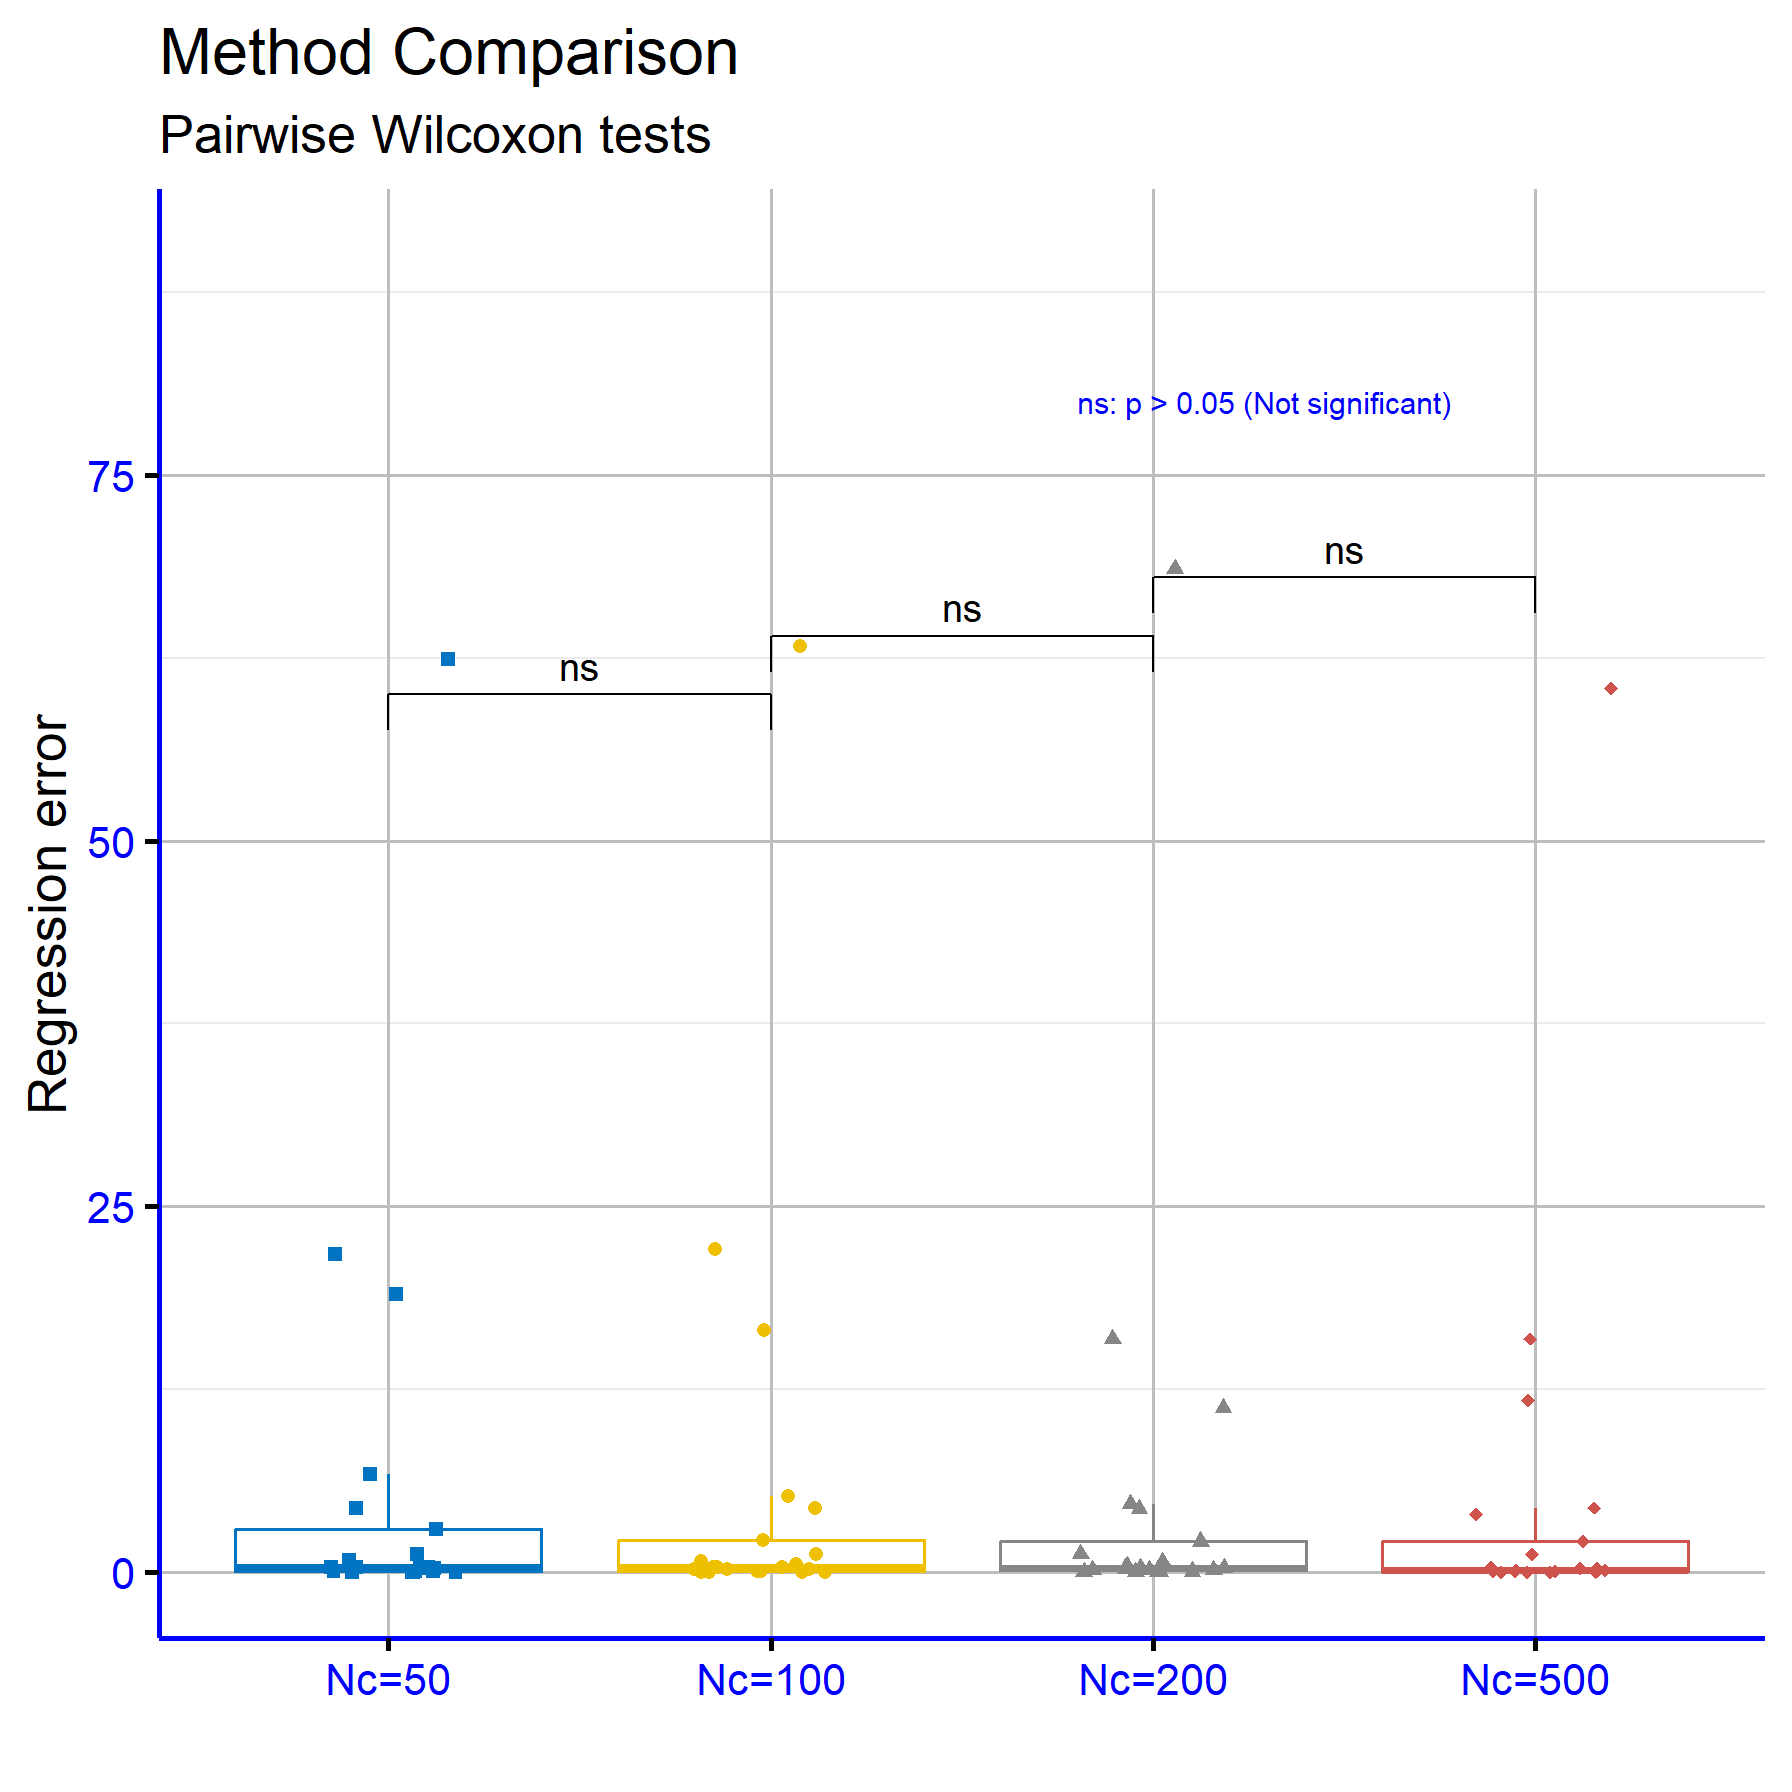
\includegraphics[scale=0.5]{stat7}
\par\end{centering}
\caption{Statistical comparison for the results obtained by the application
of the proposed method to the regression datasets using a variety
of values for the number of chromosomes $N_{c}$.\label{fig:statRegressionNC}}

\end{figure}


\subsection{Comparison with a previous work}

Recently, an improved version of the constructed neural networks was
published with the addition of a periodical application of a local
optimization procedure \citep{nn_local}. In this work a local optimization
procedure is applied to randomly selected chromosomes by maintaining
the architecture obtained by the neural network construction procedure.
In the following tables this method is denoted as INNC and a comparison
is made against the original neural network construction procedure
(denoted as NNC) and the proposed method (denoted as PROPOSED).

In Table \ref{tab:expClassOld}, the comparison of mean error rates
shows that the proposed method achieves the lowest average error rate,
19.63\%, compared to 20.92\% for INNC and 23.82\% for NNC, indicating
an overall improvement in performance. In several datasets, such as
ALCOHOL, BALANCE, CIRCULAR, DERMATOLOGY, GLASS, SEGMENT, and ZO\_NF\_S,
the proposed method clearly outperforms the others, recording substantially
lower error rates than the two comparative models. However, in certain
cases, such as HABERMAN, HEART, HOUSEVOTES, and IONOSPHERE, the proposed
method shows slightly higher error than the best-performing of the
other two models, suggesting that its superiority is not universal.
There are also instances of equivalent or marginal differences, such
as in LYMOGRAPHY and ZONF\_S, where the performances of all three
methods are very close. The overall trend indicates that the proposed
method often achieves a significant reduction in error, with improvements
being more pronounced in datasets with higher complexity or diversity
in classes.

\begin{table}[H]
\caption{Experimental results using the constructed neural networks and the
two variations for the classification datasets.\label{tab:expClassOld}}

\centering{}{\footnotesize{}%
\begin{tabular}{|c|c|c|c|}
\hline 
{\footnotesize DATASET} & {\footnotesize NNC} & INNC & {\footnotesize PROPOSED}\tabularnewline
\hline 
\hline 
{\footnotesize APPENDICITIS} & {\footnotesize 14.40\%} & 14.70\% & {\footnotesize 16.30\%}\tabularnewline
\hline 
{\footnotesize ALCOHOL} & {\footnotesize 37.72\%} & 29.79\% & {\footnotesize 20.21\%}\tabularnewline
\hline 
{\footnotesize AUSTRALIAN} & {\footnotesize 14.46\%} & 14.80\% & {\footnotesize 14.68\%}\tabularnewline
\hline 
{\footnotesize BALANCE} & {\footnotesize 23.65\%} & 8.66\% & {\footnotesize 7.26\%}\tabularnewline
\hline 
{\footnotesize CLEVELAND} & {\footnotesize 50.93\%} & 47.93\% & {\footnotesize 44.90\%}\tabularnewline
\hline 
{\footnotesize CIRCULAR} & {\footnotesize 12.66\%} & 5.32\% & {\footnotesize 4.22\%}\tabularnewline
\hline 
{\footnotesize DERMATOLOGY} & {\footnotesize 21.54\%} & 20.89\% & {\footnotesize 5.92\%}\tabularnewline
\hline 
{\footnotesize ECOLI} & {\footnotesize 49.88\%} & 48.21\% & {\footnotesize 44.79\%}\tabularnewline
\hline 
{\footnotesize GLASS} & {\footnotesize 56.09\%} & 54.24\% & {\footnotesize 49.43\%}\tabularnewline
\hline 
{\footnotesize HABERMAN} & {\footnotesize 27.53\%} & 26.70\% & {\footnotesize 28.57\%}\tabularnewline
\hline 
{\footnotesize HAYES-ROTH} & {\footnotesize 33.69\%} & 31.77\% & {\footnotesize 30.77\%}\tabularnewline
\hline 
{\footnotesize HEART} & {\footnotesize 15.67\%} & 14.74\% & {\footnotesize 17.85\%}\tabularnewline
\hline 
{\footnotesize HEARTATTACK} & {\footnotesize 20.87\%} & 20.43\% & {\footnotesize 20.67\%}\tabularnewline
\hline 
{\footnotesize HOUSEVOTES} & {\footnotesize 3.17\%} & 3.26\% & {\footnotesize 7.39\%}\tabularnewline
\hline 
{\footnotesize IONOSPHERE} & {\footnotesize 11.29\%} & 11.92\% & {\footnotesize 13.14\%}\tabularnewline
\hline 
{\footnotesize LIVERDISORDER} & {\footnotesize 32.35\%} & 31.77\% & {\footnotesize 33.38\%}\tabularnewline
\hline 
{\footnotesize LYMOGRAPHY} & {\footnotesize 25.29\%} & 25.29\% & {\footnotesize 25.14\%}\tabularnewline
\hline 
{\footnotesize MAMMOGRAPHIC} & {\footnotesize 17.62\%} & 15.81\% & {\footnotesize 17.77\%}\tabularnewline
\hline 
{\footnotesize PARKINSONS} & {\footnotesize 12.74\%} & 12.53\% & {\footnotesize 14.05\%}\tabularnewline
\hline 
{\footnotesize PIMA} & {\footnotesize 28.07\%} & 24.00\% & {\footnotesize 24.34\%}\tabularnewline
\hline 
{\footnotesize POPFAILURES} & {\footnotesize 6.98\%} & 6.44\% & {\footnotesize 7.19\%}\tabularnewline
\hline 
{\footnotesize REGIONS2} & {\footnotesize 26.18\%} & 23.18\% & {\footnotesize 25.00\%}\tabularnewline
\hline 
{\footnotesize SAHEART} & {\footnotesize 29.80\%} & 28.09\% & {\footnotesize 30.11\%}\tabularnewline
\hline 
{\footnotesize SEGMENT} & {\footnotesize 53.50\%} & 43.12\% & {\footnotesize 9.59\%}\tabularnewline
\hline 
{\footnotesize SPIRAL} & {\footnotesize 48.01\%} & 43.99\% & {\footnotesize 41.25\%}\tabularnewline
\hline 
{\footnotesize STATHEART} & {\footnotesize 18.08\%} & 18.67\% & {\footnotesize 20.26\%}\tabularnewline
\hline 
{\footnotesize STUDENT} & {\footnotesize 6.70\%} & 4.55\% & {\footnotesize 7.18\%}\tabularnewline
\hline 
{\footnotesize TRANSFUSION} & {\footnotesize 25.77\%} & 23.43\% & {\footnotesize 23.59\%}\tabularnewline
\hline 
{\footnotesize WDBC} & {\footnotesize 7.36\%} & 4.41\% & {\footnotesize 3.73\%}\tabularnewline
\hline 
{\footnotesize WINE} & {\footnotesize 13.59\%} & 9.77\% & {\footnotesize 10.41\%}\tabularnewline
\hline 
{\footnotesize Z\_F\_S} & {\footnotesize 14.53\%} & 8.53\% & {\footnotesize 6.60\%}\tabularnewline
\hline 
{\footnotesize Z\_O\_N\_F\_S} & {\footnotesize 48.62\%} & 38.58\% & {\footnotesize 49.66\%}\tabularnewline
\hline 
{\footnotesize ZO\_NF\_S} & {\footnotesize 13.54\%} & 6.84\% & {\footnotesize 3.94\%}\tabularnewline
\hline 
{\footnotesize ZONF\_S} & {\footnotesize 2.64\%} & 2.52\% & {\footnotesize 2.60\%}\tabularnewline
\hline 
{\footnotesize ZOO} & {\footnotesize 8.70\%} & 7.20\% & {\footnotesize 5.10\%}\tabularnewline
\hline 
{\footnotesize\textbf{AVERAGE}} & {\footnotesize\textbf{23.82\%}} & \textbf{20.92\%} & {\footnotesize\textbf{19.63\%}}\tabularnewline
\hline 
\end{tabular}}{\footnotesize\par}
\end{table}
In Table \ref{tab:expRegressionOld}, the comparison of mean errors
shows that INNC has the lowest average value (4.47), followed by the
proposed method (4.83) and NNC (6.29), indicating that the proposed
method demonstrates an overall improvement over NNC but falls slightly
short of INNC. In several datasets, such as AIRFOIL, CONCRETE, LASER,
PL, PLASTIC, and STOCK, the proposed method achieves the lowest or
highly competitive error values, showing clear improvement over NNC
and, in some cases, over INNC as well. However, in certain cases,
such as AUTO, BASEBALL, FRIEDMAN, LW, and SN, INNC outperforms with
lower errors, while there are also instances where NNC achieves better
performance than the proposed method, such as in DEE and FY, although
the differences are small. The overall picture indicates that the
proposed method can achieve significant improvement in specific regression
problems, but its superiority is not universal, with its performance
depending on the characteristics of each dataset.
\begin{table}[H]
\caption{Experimental results using the constructed neural networks and the
two variations on the regression datasets.\label{tab:expRegressionOld}}

\centering{}{\footnotesize{}%
\begin{tabular}{|c|c|c|c|}
\hline 
{\footnotesize DATASET} & {\footnotesize NNC} & {\footnotesize INNC} & {\footnotesize PROPOSED}\tabularnewline
\hline 
\hline 
{\footnotesize ABALONE} & {\footnotesize 5.08} & {\footnotesize 4.33} & {\footnotesize 4.41}\tabularnewline
\hline 
{\footnotesize AIRFOIL} & {\footnotesize 0.004} & {\footnotesize 0.002} & {\footnotesize 0.001}\tabularnewline
\hline 
{\footnotesize AUTO} & {\footnotesize 17.13} & {\footnotesize 11.01} & {\footnotesize 11.73}\tabularnewline
\hline 
{\footnotesize BK} & {\footnotesize 0.10} & {\footnotesize 0.07} & {\footnotesize 0.058}\tabularnewline
\hline 
{\footnotesize BL} & {\footnotesize 1.19} & {\footnotesize 0.002} & {\footnotesize 0.13}\tabularnewline
\hline 
{\footnotesize BASEBALL} & {\footnotesize 61.57} & {\footnotesize 48.42} & {\footnotesize 60.42}\tabularnewline
\hline 
{\footnotesize CONCRETE} & {\footnotesize 0.008} & {\footnotesize 0.005} & {\footnotesize 0.004}\tabularnewline
\hline 
{\footnotesize DEE} & {\footnotesize 0.26} & {\footnotesize 0.23} & {\footnotesize 0.26}\tabularnewline
\hline 
{\footnotesize FRIEDMAN} & {\footnotesize 6.29} & {\footnotesize 4.88} & {\footnotesize 1.25}\tabularnewline
\hline 
{\footnotesize FY} & {\footnotesize 0.11} & {\footnotesize 0.042} & {\footnotesize 0.13}\tabularnewline
\hline 
{\footnotesize HO} & {\footnotesize 0.015} & {\footnotesize 0.01} & {\footnotesize 0.073}\tabularnewline
\hline 
{\footnotesize HOUSING} & {\footnotesize 25.47} & {\footnotesize 16.01} & {\footnotesize 15.96}\tabularnewline
\hline 
{\footnotesize LASER} & {\footnotesize 0.025} & {\footnotesize 0.006} & {\footnotesize 0.004}\tabularnewline
\hline 
{\footnotesize LW} & {\footnotesize 0.011} & {\footnotesize 0.012} & {\footnotesize 0.32}\tabularnewline
\hline 
{\footnotesize MORTGAGE} & {\footnotesize 0.30} & {\footnotesize 0.026} & {\footnotesize 0.15}\tabularnewline
\hline 
{\footnotesize PL} & {\footnotesize 0.047} & {\footnotesize 0.022} & {\footnotesize 0.021}\tabularnewline
\hline 
{\footnotesize PLASTIC} & {\footnotesize 4.20} & {\footnotesize 2.25} & {\footnotesize 2.15}\tabularnewline
\hline 
{\footnotesize QUAKE} & {\footnotesize 0.96} & {\footnotesize 0.04} & {\footnotesize 0.061}\tabularnewline
\hline 
{\footnotesize SN} & {\footnotesize 0.026} & {\footnotesize 0.026} & {\footnotesize 0.10}\tabularnewline
\hline 
{\footnotesize STOCK} & {\footnotesize 8.92} & {\footnotesize 6.33} & {\footnotesize 3.96}\tabularnewline
\hline 
{\footnotesize TREASURY} & {\footnotesize 0.43} & {\footnotesize 0.066} & {\footnotesize 0.25}\tabularnewline
\hline 
{\footnotesize\textbf{AVERAGE}} & {\footnotesize\textbf{6.29}} & \textbf{4.47} & {\footnotesize\textbf{4.83}}\tabularnewline
\hline 
\end{tabular}}{\footnotesize\par}
\end{table}

Figure \ref{fig:statClassOld} presents the significance levels resulting
from the comparisons of error rates on classification datasets for
the proposed machine learning method in relation to the NNC and INNC
models. The comparison between NNC and INNC shows extremely high statistical
significance (p={*}{*}), indicating a clear superiority of INNC. The
comparison between NNC and the proposed method also shows a statistically
significant difference (p=), indicating that the proposed method outperforms
NNC. In contrast, the comparison between INNC and the proposed method
does not show a statistically significant difference (p=ns), suggesting
that the two methods perform similarly on these datasets.

\begin{figure}[H]
\begin{centering}
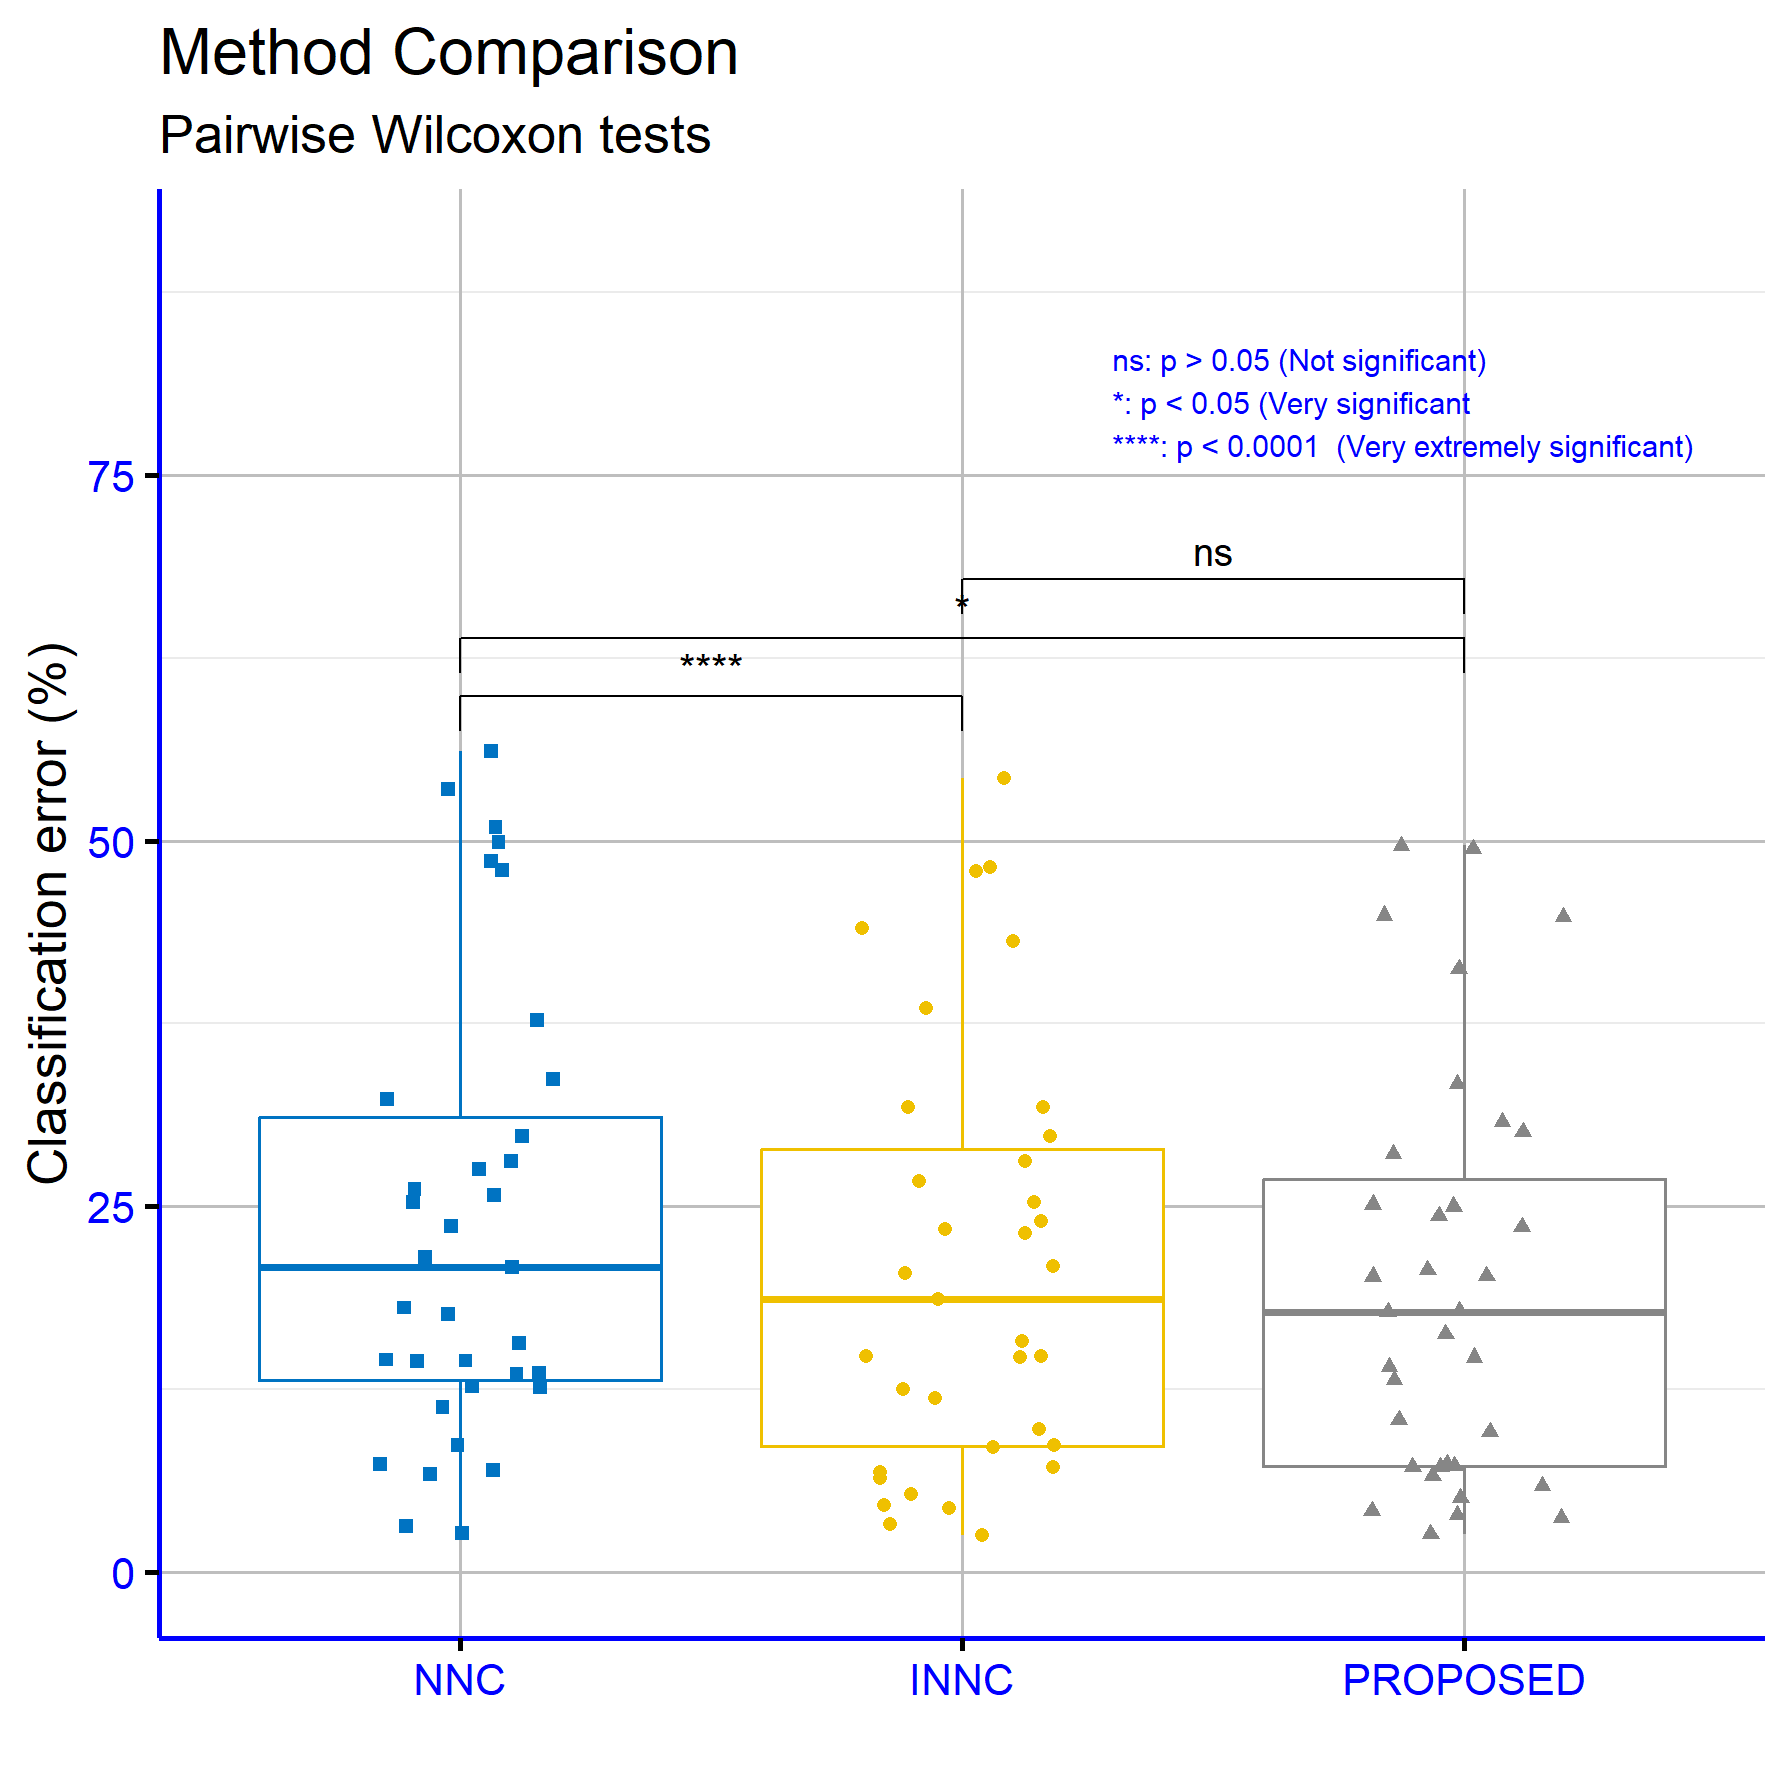
\includegraphics[scale=0.5]{stat8}
\par\end{centering}
\caption{Statistical comparison for the experimental results on the classification
datasets using the original neural construction method and the two
variations.\label{fig:statClassOld}}

\end{figure}
Figure \ref{fig:statRegressionOld} presents the significance levels
from the comparisons of error rates on classification datasets for
the proposed machine learning method in relation to the NNC and INNC
models. The comparison between NNC and INNC shows high statistical
significance (p={*}), indicating a clear superiority of INNC. The
comparison between NNC and the proposed method also shows a statistically
significant difference (p=), demonstrating the improvement of the
proposed method over NNC. In contrast, the comparison between INNC
and the proposed method does not show a statistically significant
difference (p=ns), indicating that the two methods have comparable
performance on these datasets.

\begin{figure}[H]
\begin{centering}
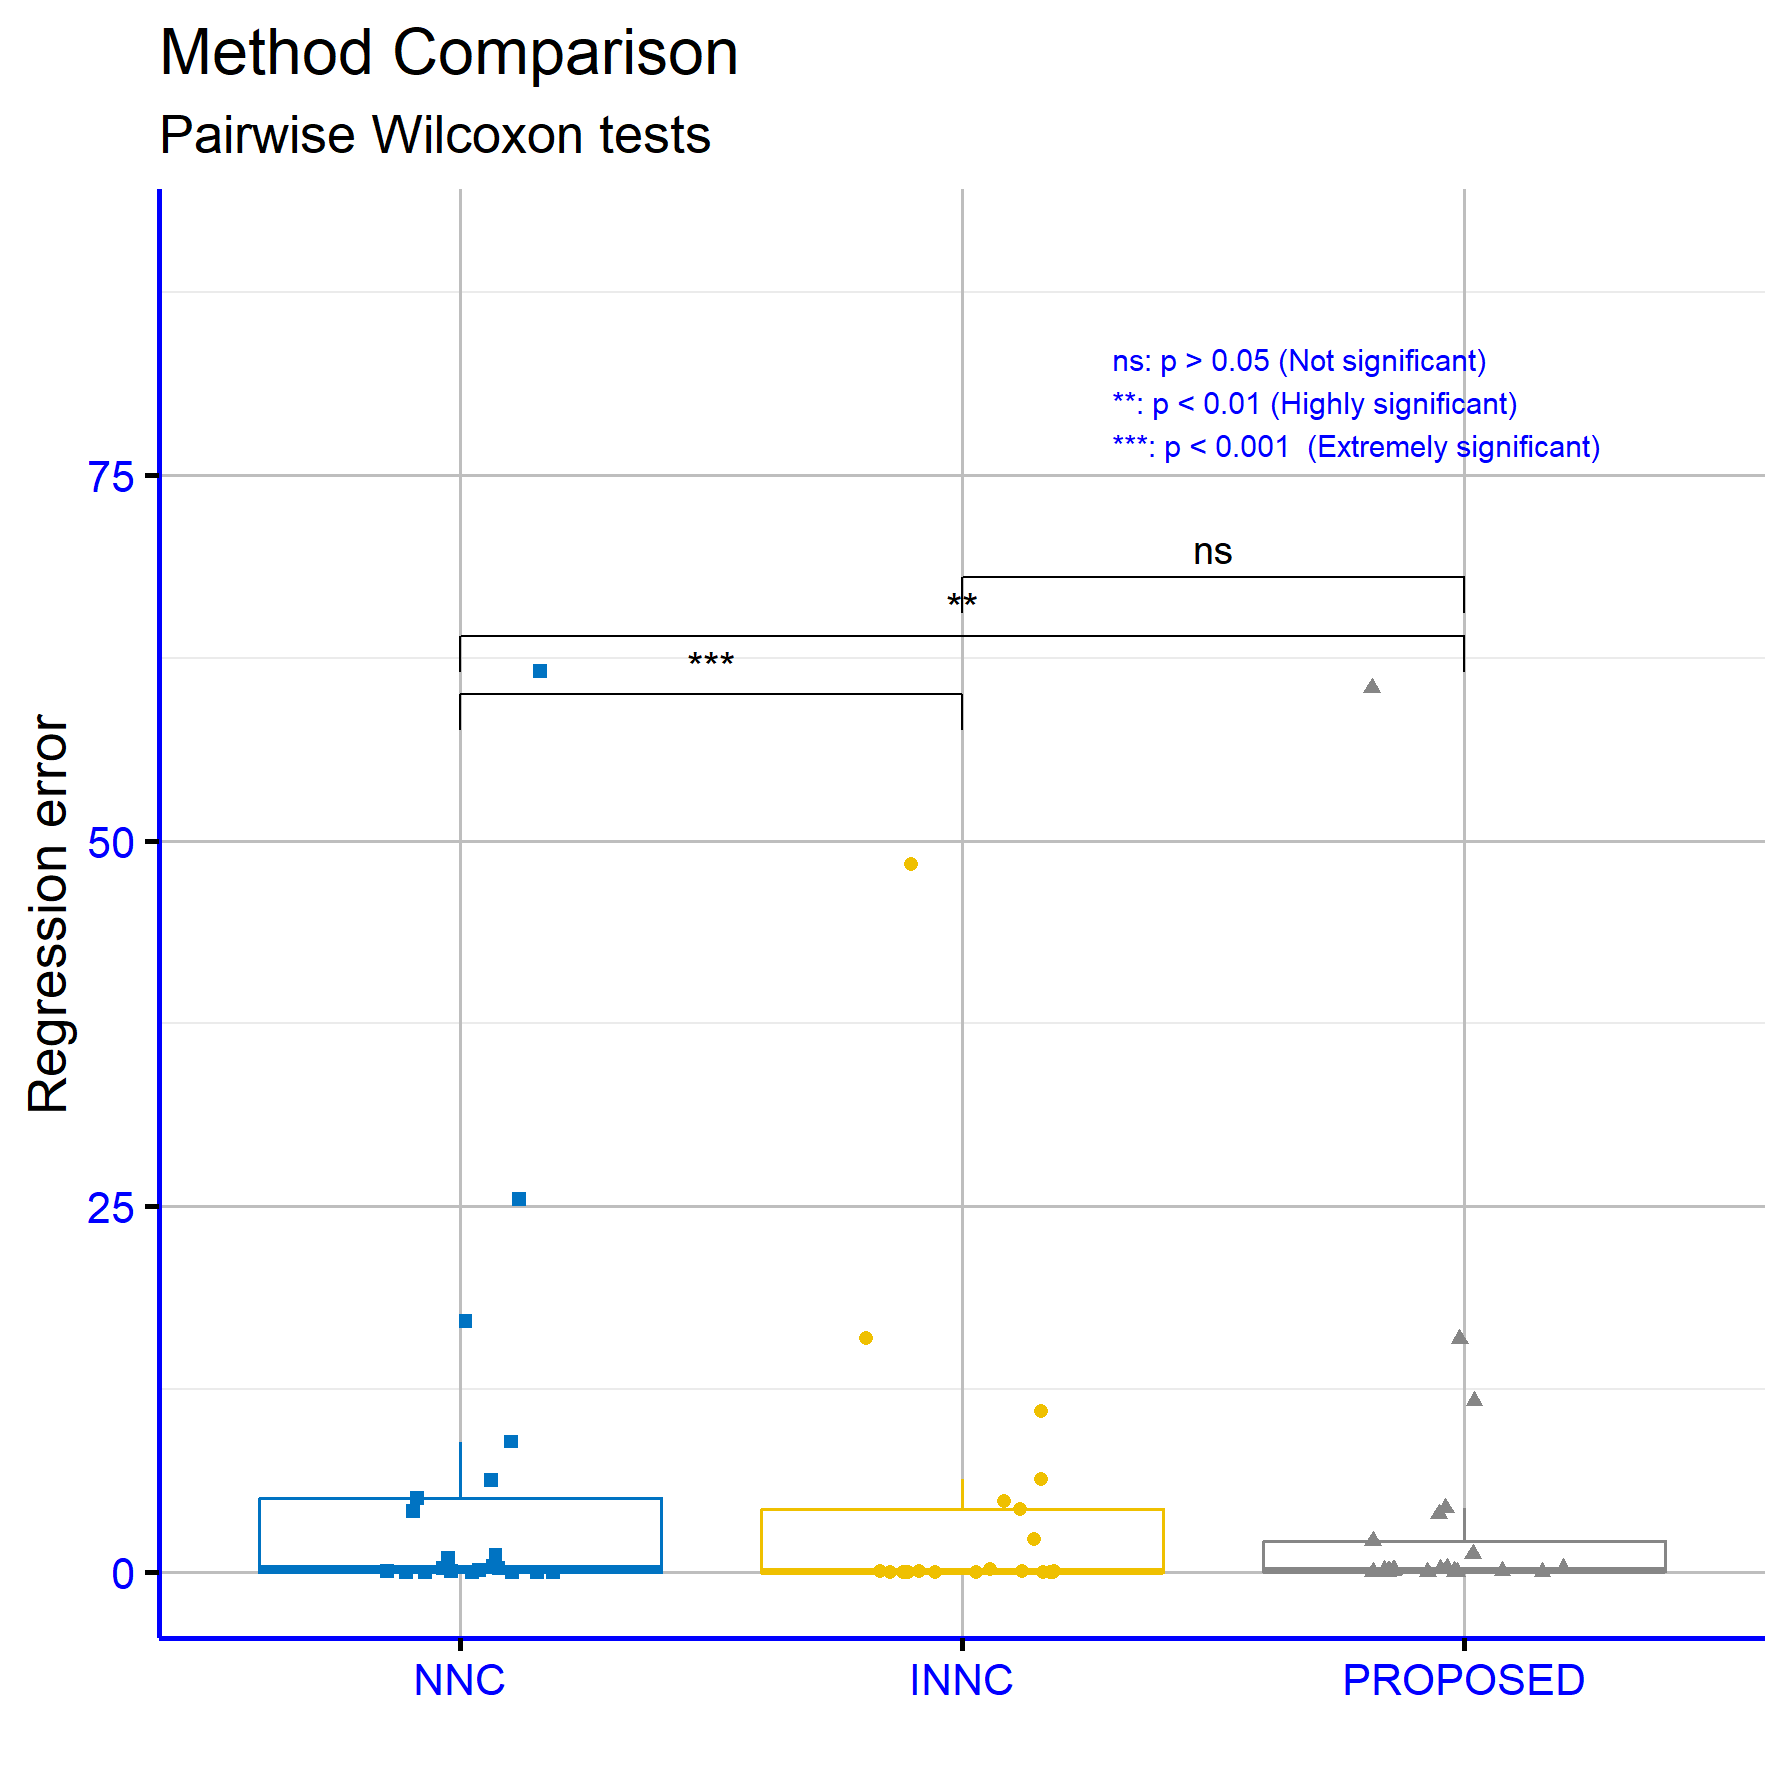
\includegraphics[scale=0.5]{stat9}
\par\end{centering}
\caption{Statistical comparison for the results obtained by the proposed method
and the two variations on the regression datasets,\label{fig:statRegressionOld}}

\end{figure}
Also, should be noted that the INNC method requires significant more
time than the proposed method, since it applies several applications
of the local search procedure on randomly selected chromosomes.

\section{Conclusions\label{sec:Conclusions}}

This study clearly demonstrates the importance of integrating a preliminary
training phase into the grammar-based evolution framework for constructing
artificial neural networks. The role of this pretraining phase extends
far beyond merely initializing the solution space. It effectively
enhances the quality of the initial population by transferring information
from a previously trained neural network, resulting in a better-informed
starting point for the evolutionary process. This enriched initialization
improves convergence rates and reduces the risk of stagnation in local
minima, especially in complex, non-linear, or noisy problem domains.

Experimental findings show that the proposed approach not only achieves
improved numerical performance metrics but also exhibits increased
consistency across diverse datasets. Unlike many conventional methods
that are often sensitive to the nature of the data and prone to high
variability in performance, the proposed model demonstrates both robustness
and generalization capability. This makes it a strong candidate for
applications in high-stakes or real-time environments where model
reliability is critical, such as medical diagnosis, energy forecasting,
or financial decision-making.

The sensitivity analysis concerning the initialization factor ($I_{w}$)
offers further insight into the behavior of the proposed model. Although
the differences among parameter values are not statistically significant,
a consistent trend toward improved accuracy with higher Iw values
suggests that careful tuning of initialization can have a meaningful
impact on model effectiveness. In more complex datasets, higher $I_{w}$
settings appear to support better generalization, pointing to the
potential of initialization strategies as a lever for optimization.

Overall, the proposed system should not be viewed as a minor variation
on existing grammar evolution techniques, but rather as a substantial
advancement in how prior knowledge and pretraining experience can
be exploited to improve and accelerate evolutionary learning. This
approach merges the advantages of pretraining with the adaptability
of evolutionary search, forming a solid foundation for future developments
involving hybrid or meta-intelligent strategies in automated neural
architecture design. Its demonstrated performance, adaptability, and
potential for integration with broader machine learning paradigms
mark it as a promising direction for ongoing and future exploration.

Regarding future research directions, there are several promising
avenues to explore. One potential extension of the current study could
involve the use of alternative pretraining techniques beyond genetic
algorithms, such as particle swarm optimization or differential evolution,
to assess the influence of various optimization strategies on the
initial population. Additionally, it would be valuable to examine
the role of the pretraining phase in relation to variables such as
the number of nodes, the level of noise in the data, and feature heterogeneity.

Finally, it is suggested that reinforcement learning techniques or
even hybrid models such as GANs and Autoencoders be incorporated into
the grammar-based evolution framework. Combining the proposed pretraining
phase with neural architecture search methodologies could lead to
even more efficient and generalizable models. The demonstrated stability
and adaptability of the proposed approach make it a strong candidate
for application in demanding real-world domains such as healthcare,
energy, and financial forecasting.

\vspace{6pt}


\authorcontributions{V.C. and I.G.T. conducted the experiments, employing several datasets
and provided the comparative experiments. D.T. and V.C. performed
the statistical analysis and prepared the manuscript. All authors
have read and agreed to the published version of the manuscript.}

\funding{This research has been financed by the European Union : Next Generation
EU through the Program Greece 2.0 National Recovery and Resilience
Plan , under the call RESEARCH -- CREATE -- INNOVATE, project name
“iCREW: Intelligent small craft simulator for advanced crew training
using Virtual Reality techniques\textquotedbl{} (project code:TAEDK-06195).}

\institutionalreview{Not applicable.}

\informedconsent{Not applicable.}

\dataavailability{Not applicable.}

\conflictsofinterest{The authors declare no conflicts of interest.}


\begin{adjustwidth}{-\extralength}{0cm}{}

\reftitle{References}
\begin{thebibliography}{99}
\bibitem[(2018)]{nn1}Abiodun, O. I., Jantan, A., Omolara, A. E.,
Dada, K. V., Mohamed, N. A., \& Arshad, H. (2018). State-of-the-art
in artificial neural network applications: A survey. Heliyon, 4(11).

\bibitem{nn2}Suryadevara, S., \& Yanamala, A. K. Y. (2021). A Comprehensive
Overview of Artificial Neural Networks: Evolution, Architectures,
and Applications. Revista de Inteligencia Artificial en Medicina,
12(1), 51-76.

\bibitem{nn_image}M. Egmont-Petersen, D. de Ridder, H. Handels, Image
processing with neural networks---a review, Pattern Recognition \textbf{35},
pp. 2279-2301, 2002.

\bibitem{nn_timeseries}G.Peter Zhang, Time series forecasting using
a hybrid ARIMA and neural network model, Neurocomputing \textbf{50},
pp. 159-175, 2003.

\bibitem{nn_credit}Z. Huang, H. Chen, C.-Jung Hsu, W.-Hwa Chen, S.
Wu, Credit rating analysis with support vector machines and neural
networks: a market comparative study, Decision Support Systems \textbf{37},
pp. 543-558, 2004.

\bibitem{nnphysics1}P. Baldi, K. Cranmer, T. Faucett et al, Parameterized
neural networks for high-energy physics, Eur. Phys. J. C \textbf{76},
2016.

\bibitem{nnphysics2}Baldi, P., Cranmer, K., Faucett, T., Sadowski,
P., \& Whiteson, D. (2016). Parameterized neural networks for high-energy
physics. The European Physical Journal C, 76(5), 1-7.

\bibitem{nn_flood}M.B. Kia, S. Pirasteh, B. Pradhan B. et al, An
artificial neural network model for flood simulation using GIS: Johor
River Basin, Malaysia, Environ Earth Sci \textbf{67}, pp. 251--264,
2012.

\bibitem{nn_solar}A.K. Yadav, S.S. Chandel, Solar radiation prediction
using Artificial Neural Network techniques: A review, Renewable and
Sustainable Energy Reviews \textbf{33}, pp. 772-781, 2014.

\bibitem{nn_agro}M.A. Getahun, S.M. Shitote, C. Zachary, Artificial
neural network based modelling approach for strength prediction of
concrete incorporating agricultural and construction wastes, Construction
and Building Materials \textbf{190}, pp. 517-525, 2018.

\bibitem{nn_wireless}M. Chen, U. Challita, W. Saad, C. Yin and M.
Debbah, Artificial Neural Networks-Based Machine Learning for Wireless
Networks: A Tutorial, IEEE Communications Surveys \& Tutorials \textbf{21},
pp. 3039-3071, 2019.

\bibitem{nn_mech1}K. Peta, J. Żurek, Prediction of air leakage in
heat exchangers for automotive applications using artificial neural
networks, In: 2018 9th IEEE Annual Ubiquitous Computing, Electronics
\& Mobile Communication Conference (UEMCON), New York, NY, USA, pp.
721-725, 2018.

\bibitem{bpnn1}Vora, K., \& Yagnik, S. (2014). A survey on backpropagation
algorithms for feedforward neural networks. International Journal
of Engineering Development and Research, 1(3), 193-197.

\bibitem{bpnn2}K. Vora, S. Yagnik, A survey on backpropagation algorithms
for feedforward neural networks, International Journal of Engineering
Development and Research \textbf{1}, pp. 193-197, 2014.

\bibitem{rpropnn-1}Pajchrowski, T., Zawirski, K., \& Nowopolski,
K. (2014). Neural speed controller trained online by means of modified
RPROP algorithm. IEEE transactions on industrial informatics, 11(2),
560-568.

\bibitem{rpropnn-2}Hermanto, R. P. S., \& Nugroho, A. (2018). Waiting-time
estimation in bank customer queues using RPROP neural networks. Procedia
Computer Science, 135, 35-42.

\bibitem{geneticnn1}Reynolds, J., Rezgui, Y., Kwan, A., \& Piriou,
S. (2018). A zone-level, building energy optimisation combining an
artificial neural network, a genetic algorithm, and model predictive
control. Energy, 151, 729-739.

\bibitem{psonn}Das, G., Pattnaik, P. K., \& Padhy, S. K. (2014).
Artificial neural network trained by particle swarm optimization for
non-linear channel equalization. Expert Systems with Applications,
41(7), 3491-3496.

\bibitem{nn_siman}Sexton, R. S., Dorsey, R. E., \& Johnson, J. D.
(1999). Beyond backpropagation: using simulated annealing for training
neural networks. Journal of Organizational and End User Computing
(JOEUC), 11(3), 3-10.

\bibitem{weight_de1}Wang, L., Zeng, Y., \& Chen, T. (2015). Back
propagation neural network with adaptive differential evolution algorithm
for time series forecasting. Expert Systems with Applications, 42(2),
855-863.

\bibitem{nn_abc}Karaboga, D., \& Akay, B. (2007, June). Artificial
bee colony (ABC) algorithm on training artificial neural networks.
In 2007 IEEE 15th Signal Processing and Communications Applications
(pp. 1-4). IEEE.

\bibitem{tabunn}R.S. Sexton, B. Alidaee, R.E. Dorsey, J.D. Johnson,
Global optimization for artificial neural networks: A tabu search
application. European Journal of Operational Research \textbf{106},
pp. 570-584, 1998.

\bibitem{nn_hybrid}J.-R. Zhang, J. Zhang, T.-M. Lok, M.R. Lyu, A
hybrid particle swarm optimization--back-propagation algorithm for
feedforward neural network training, Applied Mathematics and Computation
\textbf{185}, pp. 1026-1037, 2007.

\bibitem{nn_cascade}G. Zhao, T. Wang, Y. Jin, C. Lang, Y. Li, H.
Ling, The Cascaded Forward algorithm for neural network training,
Pattern Recognition \textbf{161}, 111292, 2025.

\bibitem{nn_gpu1}K-Su Oh, K. Jung, GPU implementation of neural networks,
Pattern Recognition \textbf{37}, pp. 1311-1314, 2004.

\bibitem{nn_gpu2}M. Zhang, K. Hibi, J. Inoue, GPU-accelerated artificial
neural network potential for molecular dynamics simulation, Computer
Physics Communications \textbf{285}, 108655, 2023.

\bibitem{nnsharing1}S.J. Nowlan and G.E. Hinton, Simplifying neural
networks by soft weight sharing, Neural Computation 4, pp. 473-493,
1992.

\bibitem{nnsharing2}Nowlan, S. J., \& Hinton, G. E. (2018). Simplifying
neural networks by soft weight sharing. In The mathematics of generalization
(pp. 373-394). CRC Press.

\bibitem{nnprunning1}S.J. Hanson and L.Y. Pratt, Comparing biases
for minimal network construction with back propagation, In D.S. Touretzky
(Ed.), Advances in Neural Information Processing Systems, Volume 1,
pp. 177-185, San Mateo, CA: Morgan Kaufmann, 1989.

\bibitem{nnprunning2}M. Augasta and T. Kathirvalavakumar, Pruning
algorithms of neural networks --- a comparative study, Central European
Journal of Computer Science, 2003.

\bibitem{nnearly1}Lutz Prechelt, Automatic early stopping using cross
validation: quantifying the criteria, Neural Networks \textbf{11},
pp. 761-767, 1998.

\bibitem{nnearly2}X. Wu and J. Liu, A New Early Stopping Algorithm
for Improving Neural Network Generalization, 2009 Second International
Conference on Intelligent Computation Technology and Automation, Changsha,
Hunan, 2009, pp. 15-18.

\bibitem{nndecay1}N. K. Treadgold and T. D. Gedeon, Simulated annealing
and weight decay in adaptive learning: the SARPROP algorithm,IEEE
Transactions on Neural Networks \textbf{9}, pp. 662-668, 1998.

\bibitem{nndecay2}M. Carvalho and T. B. Ludermir, Particle Swarm
Optimization of Feed-Forward Neural Networks with Weight Decay, 2006
Sixth International Conference on Hybrid Intelligent Systems (HIS'06),
Rio de Janeiro, Brazil, 2006, pp. 5-5.

\bibitem{nn_arch1}J. Arifovic, R. Gençay, Using genetic algorithms
to select architecture of a feedforward artificial neural network,
Physica A: Statistical Mechanics and its Applications \textbf{289},
pp. 574-594, 2001.

\bibitem{nn_arch2}P.G. Benardos, G.C. Vosniakos, Optimizing feedforward
artificial neural network architecture, Engineering Applications of
Artificial Intelligence \textbf{20}, pp. 365-382, 2007.

\bibitem{nn_arch3}B.A. Garro, R.A. Vázquez, Designing Artificial
Neural Networks Using Particle Swarm Optimization Algorithms, Computational
Intelligence and Neuroscience, 369298, 2015. 

\bibitem[(2001)]{nn_ereinf}Siebel, N. T., \& Sommer, G. (2007). Evolutionary
reinforcement learning of artificial neural networks. International
Journal of Hybrid Intelligent Systems, 4(3), 171-183.

\bibitem[(2001)]{nn_reinf}Jaafra, Y., Laurent, J. L., Deruyver, A.,
\& Naceur, M. S. (2019). Reinforcement learning for neural architecture
search: A review. Image and Vision Computing, 89, 57-66.

\bibitem[(2001)]{nn_param_sharing}Pham, H., Guan, M., Zoph, B., Le,
Q., \& Dean, J. (2018, July). Efficient neural architecture search
via parameters sharing. In International conference on machine learning
(pp. 4095-4104). PMLR.

\bibitem[(2001)]{nn_snas}Xie, S., Zheng, H., Liu, C., \& Lin, L.
(2018). SNAS: stochastic neural architecture search. arXiv preprint
arXiv:1812.09926.

\bibitem[(2001)]{nn_bayes}Zhou, H., Yang, M., Wang, J., \& Pan, W.
(2019, May). Bayesnas: A bayesian approach for neural architecture
search. In International conference on machine learning (pp. 7603-7613).
PMLR.

\bibitem{ge1}M. O’Neill, C. Ryan, Grammatical evolution, IEEE Trans.
Evol. Comput. \textbf{5,}pp. 349--358, 2001.

\bibitem{nnc}I.G. Tsoulos, D. Gavrilis, E. Glavas, Neural network
construction and training using grammatical evolution, Neurocomputing
\textbf{72}, pp. 269-277, 2008.

\bibitem{nnc_amide1}G.V. Papamokos, I.G. Tsoulos, I.N. Demetropoulos,
E. Glavas, Location of amide I mode of vibration in computed data
utilizing constructed neural networks, Expert Systems with Applications
\textbf{36}, pp. 12210-12213, 2009.

\bibitem{nnc_de}I.G. Tsoulos, D. Gavrilis, E. Glavas, Solving differential
equations with constructed neural networks, Neurocomputing \textbf{72},
pp. 2385-2391, 2009.

\bibitem{nnc_feas}I.G. Tsoulos, G. Mitsi, A. Stavrakoudis, S. Papapetropoulos,
Application of Machine Learning in a Parkinson's Disease Digital Biomarker
Dataset Using Neural Network Construction (NNC) Methodology Discriminates
Patient Motor Status, Frontiers in ICT 6, 10, 2019.

\bibitem{nnc_student}V. Christou, I.G. Tsoulos, V. Loupas, A.T. Tzallas,
C. Gogos, P.S. Karvelis, N. Antoniadis, E. Glavas, N. Giannakeas,
Performance and early drop prediction for higher education students
using machine learning, Expert Systems with Applications \textbf{225},
120079, 2023.

\bibitem{nnc_autism}E.I. Toki, J. Pange, G. Tatsis, K. Plachouras,
I.G. Tsoulos, Utilizing Constructed Neural Networks for Autism Screening,
Applied Sciences \textbf{14}, 3053, 2024.

\bibitem[(1993)]{pre_bp}Li, G., Alnuweiri, H., Wu, Y., \& Li, H.
(1993, March). Acceleration of back propagation through initial weight
pre-training with delta rule. In IEEE International Conference on
neural networks (pp. 580-585). IEEE.

\bibitem[(2010)]{pre_erhan}Erhan, D., Courville, A., Bengio, Y.,
\& Vincent, P. (2010, March). Why does unsupervised pre-training help
deep learning?. In Proceedings of the thirteenth international conference
on artificial intelligence and statistics (pp. 201-208). JMLR Workshop
and Conference Proceedings.

\bibitem[(1993)]{pre_soft}Owhadi-Kareshk, M., Sedaghat, Y., \& Akbarzadeh-T,
M. R. (2017, October). Pre-training of an artificial neural network
for software fault prediction. In 2017 7th International Conference
on Computer and Knowledge Engineering (ICCKE) (pp. 223-228). IEEE.

\bibitem[(1993)]{pre_regression}Saikia, P., Vij, P., \& Baruah, R.
D. (2018, July). Unsupervised pre-training on improving the performance
of neural network in regression. In 2018 International Joint Conference
on Neural Networks (IJCNN) (pp. 01-06). IEEE.

\bibitem[(1993)]{pre_reduction}Kroshchanka, A., \& Golovko, V. (2021,
September). The reduction of fully connected neural network parameters
using the pre-training technique. In 2021 11th IEEE International
Conference on Intelligent Data Acquisition and Advanced Computing
Systems: Technology and Applications (IDAACS) (Vol. 2, pp. 937-941).
IEEE.

\bibitem[(1993)]{pre_extreme}Noinongyao, P., \& Watchareeruetai,
U. (2018, December). An extreme learning machine based pretraining
method for multi-layer neural networks. In 2018 Joint 10th International
Conference on Soft Computing and Intelligent Systems (SCIS) and 19th
International Symposium on Advanced Intelligent Systems (ISIS) (pp.
608-613). IEEE.

\bibitem{Holland} Holland, J.H. Genetic algorithms. Sci. Am. 1992,
267, 66--73.

\bibitem{Stender} Stender, J. Parallel Genetic Algorithms: Theory
\& Applications; IOS Press: Amsterdam, The Netherlands, 1993.

\bibitem{Goldberg} Goldberg, D. Genetic Algorithms in Search, Optimization
and Machine Learning; Addison-Wesley Publishing Company: Reading,
MA, USA, 1989.

\bibitem{Michaelewicz} Michaelewicz, Z. Genetic Algorithms + Data
Structures = Evolution Programs; Springer: Berlin/Heidelberg, Germany,
1996.

\bibitem{Liu}Liu, X.; Jiang, D.; Tao, B.; Jiang, G.; Sun, Y.; Kong,
J.; Chen, B. Genetic algorithm-based trajectory optimization for digital
twin robots. Front. Bioeng. Biotechnol. 2022, 9, 793782.

\bibitem{Chen} Chen, Q.; Hu, X. Design of intelligent control system
for agricultural greenhouses based on adaptive improved genetic algorithm
for multi-energy supply system. Energy Rep. 2022, 8, 12126--12138.

\bibitem[(1989)]{Hornik}Hornik, K.; Stinchcombe, M.; White, H. Multilayer
feedforward networks are universal approximators. Neural Netw. 1989,
2, 359--366. 

\bibitem{Min} Min, D.; Song, Z.; Chen, H.; Wang, T.; Zhang, T. Genetic
algorithm optimized neural network based fuel cell hybrid electric
vehicle energy management strategy under start-stop condition. Appl.
Energy 2022, 306, 118036

\bibitem{kaelo}P. Kaelo, M.M. Ali, Integrated crossover rules in
real coded genetic algorithms, European Journal of Operational Research
\textbf{176}, pp. 60-76, 2007.

\bibitem{bnf1}J. W. Backus. The Syntax and Semantics of the Proposed
International Algebraic Language of the Zurich ACM-GAMM Conference.
Proceedings of the International Conference on Information Processing,
UNESCO, 1959, pp.125-132.

\bibitem{ge_program1}C. Ryan, J. Collins, M. O’Neill, Grammatical
evolution: Evolving programs for an arbitrary language. In: Banzhaf,
W., Poli, R., Schoenauer, M., Fogarty, T.C. (eds) Genetic Programming.
EuroGP 1998. Lecture Notes in Computer Science, vol 1391. Springer,
Berlin, Heidelberg, 1998.

\bibitem{ge_program2}M. O’Neill, M., C. Ryan, Evolving Multi-line
Compilable C Programs. In: Poli, R., Nordin, P., Langdon, W.B., Fogarty,
T.C. (eds) Genetic Programming. EuroGP 1999. Lecture Notes in Computer
Science, vol 1598. Springer, Berlin, Heidelberg, 1999.

\bibitem{ge_music}A.O. Puente, R. S. Alfonso, M. A. Moreno, Automatic
composition of music by means of grammatical evolution, In: APL '02:
Proceedings of the 2002 conference on APL: array processing languages:
lore, problems, and applications July 2002 Pages 148--155. 

\bibitem{ge_pacman}E. Galván-López, J.M. Swafford, M. O’Neill, A.
Brabazon, Evolving a Ms. PacMan Controller Using Grammatical Evolution.
In: , et al. Applications of Evolutionary Computation. EvoApplications
2010. Lecture Notes in Computer Science, vol 6024. Springer, Berlin,
Heidelberg, 2010.

\bibitem{ge_supermario}N. Shaker, M. Nicolau, G. N. Yannakakis, J.
Togelius, M. O'Neill, Evolving levels for Super Mario Bros using grammatical
evolution, 2012 IEEE Conference on Computational Intelligence and
Games (CIG), 2012, pp. 304-31.

\bibitem{ge_energy}D. Martínez-Rodríguez, J. M. Colmenar, J. I. Hidalgo,
R.J. Villanueva Micó, S. Salcedo-Sanz, Particle swarm grammatical
evolution for energy demand estimation, Energy Science and Engineering
\textbf{8}, pp. 1068-1079, 2020.

\bibitem{ge_crypt}C. Ryan, M. Kshirsagar, G. Vaidya, G. et al. Design
of a cryptographically secure pseudo random number generator with
grammatical evolution. Sci Rep \textbf{12}, 8602, 2022.

\bibitem{ge_trading}C. Martín, D. Quintana, P. Isasi, Grammatical
Evolution-based ensembles for algorithmic trading, Applied Soft Computing
\textbf{84}, 105713, 2019.

\bibitem[(1989)]{uci} M. Kelly, R. Longjohn, K. Nottingham, The UCI
Machine Learning Repository, https://archive.ics.uci.edu.

\bibitem{Keel}J. Alcalá-Fdez, A. Fernandez, J. Luengo, J. Derrac,
S. García, L. Sánchez, F. Herrera. KEEL Data-Mining Software Tool:
Data Set Repository, Integration of Algorithms and Experimental Analysis
Framework. Journal of Multiple-Valued Logic and Soft Computing 17,
pp. 255-287, 2011.

\bibitem{appendicitis}Weiss, Sholom M. and Kulikowski, Casimir A.,
Computer Systems That Learn: Classification and Prediction Methods
from Statistics, Neural Nets, Machine Learning, and Expert Systems,
Morgan Kaufmann Publishers Inc, 1991.

\bibitem[Tzimourta(2018)]{alcohol}Tzimourta, K.D.; Tsoulos, I.; Bilero,
I.T.; Tzallas, A.T.; Tsipouras, M.G.; Giannakeas, N. Direct Assessment
of Alcohol Consumption in Mental State Using Brain Computer Interfaces
and Grammatical Evolution. Inventions 2018, 3, 51.

\bibitem[Quinlan(2018)]{australian}J.R. Quinlan, Simplifying Decision
Trees. International Journal of Man-Machine Studies \textbf{27}, pp.
221-234, 1987. 

\bibitem{balance}T. Shultz, D. Mareschal, W. Schmidt, Modeling Cognitive
Development on Balance Scale Phenomena, Machine Learning \textbf{16},
pp. 59-88, 1994.

\bibitem[(2004)]{cleveland1}Z.H. Zhou,Y. Jiang, NeC4.5: neural ensemble
based C4.5,\textquotedbl{} in IEEE Transactions on Knowledge and Data
Engineering \textbf{16}, pp. 770-773, 2004.

\bibitem{cleveland2}R. Setiono , W.K. Leow, FERNN: An Algorithm for
Fast Extraction of Rules from Neural Networks, Applied Intelligence
\textbf{12}, pp. 15-25, 2000.

\bibitem[(1998)]{dermatology}G. Demiroz, H.A. Govenir, N. Ilter,
Learning Differential Diagnosis of Eryhemato-Squamous Diseases using
Voting Feature Intervals, Artificial Intelligence in Medicine. \textbf{13},
pp. 147--165, 1998.

\bibitem[(1996)]{ecoli}P. Horton, K.Nakai, A Probabilistic Classification
System for Predicting the Cellular Localization Sites of Proteins,
In: Proceedings of International Conference on Intelligent Systems
for Molecular Biology \textbf{4}, pp. 109-15, 1996.

\bibitem[(1977)]{hayes-roth}B. Hayes-Roth, B., F. Hayes-Roth. Concept
learning and the recognition and classification of exemplars. Journal
of Verbal Learning and Verbal Behavior \textbf{16}, pp. 321-338, 1977.

\bibitem[(1997)]{heart}I. Kononenko, E. Šimec, M. Robnik-Šikonja,
Overcoming the Myopia of Inductive Learning Algorithms with RELIEFF,
Applied Intelligence \textbf{7}, pp. 39--55, 1997

\bibitem[(2002)]{housevotes}R.M. French, N. Chater, Using noise to
compute error surfaces in connectionist networks: a novel means of
reducing catastrophic forgetting, Neural Comput. \textbf{14}, pp.
1755-1769, 2002.

\bibitem[(2004)]{ion1}J.G. Dy , C.E. Brodley, Feature Selection for
Unsupervised Learning, The Journal of Machine Learning Research \textbf{5},
pp 845--889, 2004.

\bibitem{ion2}S. J. Perantonis, V. Virvilis, Input Feature Extraction
for Multilayered Perceptrons Using Supervised Principal Component
Analysis, Neural Processing Letters \textbf{10}, pp 243--252, 1999.

\bibitem[(2002)]{liver} J. Garcke, M. Griebel, Classification with
sparse grids using simplicial basis functions, Intell. Data Anal.
\textbf{6}, pp. 483-502, 2002.

\bibitem{liver1}J. Mcdermott, R.S. Forsyth, Diagnosing a disorder
in a classification benchmark, Pattern Recognition Letters \textbf{73},
pp. 41-43, 2016.

\bibitem[(2002)]{lymography}G. Cestnik, I. Konenenko, I. Bratko,
Assistant-86: A Knowledge-Elicitation Tool for Sophisticated Users.
In: Bratko, I. and Lavrac, N., Eds., Progress in Machine Learning,
Sigma Press, Wilmslow, pp. 31-45, 1987. 

\bibitem[(2007)]{mammographic}M. Elter, R. Schulz-Wendtland, T. Wittenberg,
The prediction of breast cancer biopsy outcomes using two CAD approaches
that both emphasize an intelligible decision process, Med Phys. \textbf{34},
pp. 4164-72, 2007.

\bibitem[(2007)]{parkinsons1}M.A. Little, P.E. McSharry, S.J Roberts
et al, Exploiting Nonlinear Recurrence and Fractal Scaling Properties
for Voice Disorder Detection. BioMed Eng OnLine \textbf{6}, 23, 2007.

\bibitem{parkinsons2}M.A. Little, P.E. McSharry, E.J. Hunter, J.
Spielman, L.O. Ramig, Suitability of dysphonia measurements for telemonitoring
of Parkinson's disease. IEEE Trans Biomed Eng. \textbf{56}, pp. 1015-1022,
2009.

\bibitem[(2007)]{pima}J.W. Smith, J.E. Everhart, W.C. Dickson, W.C.
Knowler, R.S. Johannes, Using the ADAP learning algorithm to forecast
the onset of diabetes mellitus, In: Proceedings of the Symposium on
Computer Applications and Medical Care IEEE Computer Society Press,
pp.261-265, 1988.

\bibitem[(2007)]{popfailures}D.D. Lucas, R. Klein, J. Tannahill,
D. Ivanova, S. Brandon, D. Domyancic, Y. Zhang, Failure analysis of
parameter-induced simulation crashes in climate models, Geoscientific
Model Development \textbf{6}, pp. 1157-1171, 2013.

\bibitem[(2007)]{regions2}N. Giannakeas, M.G. Tsipouras, A.T. Tzallas,
K. Kyriakidi, Z.E. Tsianou, P. Manousou, A. Hall, E.C. Karvounis,
V. Tsianos, E. Tsianos, A clustering based method for collagen proportional
area extraction in liver biopsy images (2015) Proceedings of the Annual
International Conference of the IEEE Engineering in Medicine and Biology
Society, EMBS, 2015-November, art. no. 7319047, pp. 3097-3100. 

\bibitem[(2007)]{saheart}T. Hastie, R. Tibshirani, Non-parametric
logistic and proportional odds regression, JRSS-C (Applied Statistics)
\textbf{36}, pp. 260--276, 1987.

\bibitem{segment}M. Dash, H. Liu, P. Scheuermann, K. L. Tan, Fast
hierarchical clustering and its validation, Data \& Knowledge Engineering
\textbf{44}, pp 109--138, 2003.

\bibitem[(2007)]{student}P. Cortez, A. M. Gonçalves Silva, Using
data mining to predict secondary school student performance, In Proceedings
of 5th FUture BUsiness TEChnology Conference (FUBUTEC 2008) (pp. 5--12).
EUROSIS-ETI, 2008.

\bibitem[(2007)]{transfusion}I-Cheng Yeh, King-Jang Yang, Tao-Ming
Ting, Knowledge discovery on RFM model using Bernoulli sequence, Expert
Systems with Applications \textbf{36}, pp. 5866-5871, 2009.

\bibitem[(2007)]{wdbc1}Jeyasingh, S., \& Veluchamy, M. (2017). Modified
bat algorithm for feature selection with the Wisconsin diagnosis breast
cancer (WDBC) dataset. Asian Pacific journal of cancer prevention:
APJCP, 18(5), 1257.

\bibitem[(2007)]{wdbc2}Alshayeji, M. H., Ellethy, H., \& Gupta, R.
(2022). Computer-aided detection of breast cancer on the Wisconsin
dataset: An artificial neural networks approach. Biomedical signal
processing and control, 71, 103141.

\bibitem[(2007)]{wine1}M. Raymer, T.E. Doom, L.A. Kuhn, W.F. Punch,
Knowledge discovery in medical and biological datasets using a hybrid
Bayes classifier/evolutionary algorithm. IEEE transactions on systems,
man, and cybernetics. Part B, Cybernetics : a publication of the IEEE
Systems, Man, and Cybernetics Society, \textbf{33} , pp. 802-813,
2003.

\bibitem{wine2}P. Zhong, M. Fukushima, Regularized nonsmooth Newton
method for multi-class support vector machines, Optimization Methods
and Software \textbf{22}, pp. 225-236, 2007.

\bibitem[(2007)]{eeg1}R. G. Andrzejak, K. Lehnertz, F.Mormann, C.
Rieke, P. David, and C. E. Elger, “Indications of nonlinear deterministic
and finite-dimensional structures in time series of brain electrical
activity: dependence on recording region and brain state,” Physical
Review E, vol. 64, no. 6, Article ID 061907, 8 pages, 2001. 

\bibitem{eeg2}A. T. Tzallas, M. G. Tsipouras, and D. I. Fotiadis,
“Automatic Seizure Detection Based on Time-Frequency Analysis and
Artificial Neural Networks,” Computational Intelligence and Neuroscience,
vol. 2007, Article ID 80510, 13 pages, 2007. doi:10.1155/2007/80510

\bibitem[(2007)]{zoo}M. Koivisto, K. Sood, Exact Bayesian Structure
Discovery in Bayesian Networks, The Journal of Machine Learning Research\textbf{
5}, pp. 549--573, 2004.

\bibitem[(2007)]{abalone}Nash, W.J.; Sellers, T.L.; Talbot, S.R.;
Cawthor, A.J.; Ford, W.B. The Population Biology of Abalone (\_Haliotis\_
species) in Tasmania. I. Blacklip Abalone (\_H. rubra\_) from the
North Coast and Islands of Bass Strait, Sea Fisheries Division; Technical
Report No. 48; Department of Primary Industry and Fisheries, Tasmania:
Hobart, Australia, 1994; ISSN 1034-3288

\bibitem[(2007)]{airfoil}Brooks, T.F.; Pope, D.S.; Marcolini, A.M.
Airfoil Self-Noise and Prediction. Technical Report, NASA RP-1218.
July 1989. Available online: https://ntrs.nasa.gov/citations/19890016302
(accessed on 14 November 2024).

\bibitem[(2007)]{concrete}I.Cheng Yeh, Modeling of strength of high
performance concrete using artificial neural networks, Cement and
Concrete Research. \textbf{28}, pp. 1797-1808, 1998. 

\bibitem{friedman}Friedman, J. (1991): Multivariate Adaptative Regression
Splines. Annals of Statistics, 19:1, 1-{}-141. 

\bibitem[(2007)]{housing}D. Harrison and D.L. Rubinfeld, Hedonic
prices and the demand for clean ai, J. Environ. Economics \& Management
\textbf{5}, pp. 81-102, 1978.

\bibitem[(2025)]{optimus}Tsoulos, I.G.; Charilogis, V.; Kyrou, G.;
Stavrou, V.N.; Tzallas, A. OPTIMUS: A Multidimensional Global Optimization
Package. J. Open Source Softw. 2025, 10, 7584.

\bibitem{nn_adam}D. P. Kingma, J. L. Ba, ADAM: a method for stochastic
optimization, in: Proceedings of the 3rd International Conference
on Learning Representations (ICLR 2015), pp. 1--15, 2015.

\bibitem{powell}M.J.D Powell, A Tolerant Algorithm for Linearly Constrained
Optimization Calculations, Mathematical Programming \textbf{45}, pp.
547-566, 1989. 

\bibitem[(1991)]{rbf1}J. Park and I. W. Sandberg, Universal Approximation
Using Radial-Basis-Function Networks, Neural Computation \textbf{3},
pp. 246-257, 1991.

\bibitem{rbf2}G.A. Montazer, D. Giveki, M. Karami, H. Rastegar, Radial
basis function neural networks: A review. Comput. Rev. J \textbf{1},
pp. 52-74, 2018.

\bibitem[(2002)]{neat}K. O. Stanley, R. Miikkulainen, Evolving Neural
Networks through Augmenting Topologies, Evolutionary Computation \textbf{10},
pp. 99-127, 2002.

\bibitem[(2002)]{prune}Zhu, V., Lu, Y., \& Li, Q. (2006). MW-OBS:
An improved pruning method for topology design of neural networks.
Tsinghua Science and Technology, 11(4), 307-312.

\bibitem{fcn}Grzegorz Klima, Fast Compressed Neural Networks, available
from \url{http://fcnn.sourceforge.net/}.

\bibitem[(2023)]{pirvision}Emad-Ud-Din, M., \& Wang, Y. (2023). Promoting
occupancy detection accuracy using on-device lifelong learning. IEEE
Sensors Journal, 23(9), 9595-9606.

\bibitem[(2024)]{beed}Banu PK, N. (2024). Feature Engineering for
Epileptic Seizure Classification Using SeqBoostNet. International
Journal of Computing and Digital Systems, 16(1), 1-14.

\bibitem[(2024)]{nn_local}Tsoulos, I.G.; Charilogis, V.; Tsalikakis,
D.; Tzallas, A. Improving the Generalization Abilities of Constructed
Neural Networks with the Addition of Local Optimization Techniques.
Algorithms 2024, 17, 446. 

\end{thebibliography}
%%%%%%%%%%%%%%%%%%%%%%%%%%%%%%%%%%%%%%%%%%
%% for journal Sci
%\reviewreports{\\
%Reviewer 1 comments and authors' response\\
%Reviewer 2 comments and authors' response\\
%Reviewer 3 comments and authors' response
%}
%%%%%%%%%%%%%%%%%%%%%%%%%%%%%%%%%%%%%%%%%%

\PublishersNote{}

\end{adjustwidth}{}
\end{document}
